% TO DO: https://tex.stackexchange.com/questions/425182/remove-initial-letter-on-similar-reference-in-apacite


%%%%%
%%
%% Sample document ``thesis.tex''
%%
%% Version: v0.2
%% Authors: Jean Martina, Rok Strnisa, Matej Urbas
%% Date: 30/07/2008
%%
%% Copyright (c) 2008-2011, Rok Strniša, Jean Martina, Matej Urbas
%% License: Simplified BSD License
%% License file: ./License
%% Original License URL: http://www.freebsd.org/copyright/freebsd-license.html
%%%%%

% Available documentclass options:
%
%   <all `report` document class options, e.g.: `a5paper`>
%   withindex   - enables the index. New index entries can be added through `\index{my entry}`
%   glossary    - enables the glossary.
%   techreport  - typesets the thesis in the technical report format.
%   firstyr     - formats the document as a first-year report.
%   times       - uses the `Times` font.
%   backrefs    - add back references in the Bibliography section
%
% For more info see `README.md`
\documentclass[withindex,glossary]{cam-thesis}


\usepackage{apacite} % bibliography
\usepackage{titlesec} % attempted to play with header spacing?
\usepackage{libertine} % main font
\usepackage{booktabs} % Provides \bottomrule I think
\usepackage[table]{xcolor} % colored rows for tables
    \definecolor{thead}{HTML}{5b9bd5}
    \definecolor{headtext}{gray}{1}
    \definecolor{trowdark}{HTML}{ddebf7}
    \definecolor{trowlight}{gray}{1}
\usepackage[labelfont=bf]{caption}
\captionsetup{justification=raggedright,singlelinecheck=false}
\usepackage{adjustbox} % Lets you coerce table width to page width
\usepackage{chngcntr} % Continuous figure/table numbering
\counterwithout{figure}{chapter}
\counterwithout{table}{chapter}
\usepackage{upgreek} % For mu in units and alpha in immuno
\usepackage{textcomp} % in-text degree and minus symbols
\usepackage{graphicx}
    \graphicspath{ {./figs/} }
\usepackage{svg} % Should use PDF instead to preserve fonts
\usepackage{lscape}

%\usepackage{fontspec}
%\setmainfont{Georgia}
\newcommand{\code}[1]{\mbox{\texttt{#1}}} % for function names
\renewcommand*{\ttdefault}{qcr} % Default was ugly


%%%%%%%%%%%%%%%%%%%%%%%%%%%%%%%%%%%%%%%%%%%%%%%%%%%%%%%%%%%%%%%%%%%%%%%%%%%%%%%%
%% Thesis meta-information
%%

%% The title of the thesis:
\title{Sox Gene Redundancy in the \emph{Drosophila} Nervous System}

%% The full name of the author (e.g.: James Smith):
\author{Edridge Kevin D'Souza}

%% College affiliation:
\college{Churchill College}

%% College shield [optional]:
% \collegeshield{CollegeShields/Christs}
 \collegeshield{CollegeShields/Churchill}
% \collegeshield{CollegeShields/Clare}
% \collegeshield{CollegeShields/ClareHall}
% \collegeshield{CollegeShields/CorpusChristi}
% \collegeshield{CollegeShields/Darwin}
% \collegeshield{CollegeShields/Downing}
% \collegeshield{CollegeShields/Emmanuel}
% \collegeshield{CollegeShields/Fitzwilliam}
% \collegeshield{CollegeShields/Girton}
% \collegeshield{CollegeShields/GonCaius}
% \collegeshield{CollegeShields/Homerton}
% \collegeshield{CollegeShields/HughesHall}
% \collegeshield{CollegeShields/Jesus}
% \collegeshield{CollegeShields/Kings}
% \collegeshield{CollegeShields/LucyCavendish}
% \collegeshield{CollegeShields/Magdalene}
% \collegeshield{CollegeShields/MurrayEdwards}
% \collegeshield{CollegeShields/Newnham}
% \collegeshield{CollegeShields/Pembroke}
% \collegeshield{CollegeShields/Peterhouse}
% \collegeshield{CollegeShields/Queens}
% \collegeshield{CollegeShields/Robinson}
% \collegeshield{CollegeShields/Selwyn}
% \collegeshield{CollegeShields/SidneySussex}
% \collegeshield{CollegeShields/StCatharines}
% \collegeshield{CollegeShields/StEdmunds}
% \collegeshield{CollegeShields/StJohns}
% \collegeshield{CollegeShields/Trinity}
% \collegeshield{CollegeShields/TrinityHall}
% \collegeshield{CollegeShields/Wolfson}
%\collegeshield{CollegeShields/FitzwilliamRed}

%% Submission date [optional]:
% \submissiondate{November, 2042}

%% You can redefine the submission notice [optional]:
% \submissionnotice{A badass thesis submitted on time for the Degree of PhD}

%% Declaration date:
\date{September 2020}

%% PDF meta-info:
\subjectline{Genetics}
\keywords{Drosophila neurodevelopment Sox SoxNeuro SoxN Dichaete bioinformatics genomics}



%%%%%%%%%%%%%%%%%%%%%%%%%%%%%%%%%%%%%%%%%%%%%%%%%%%%%%%%%%%%%%%%%%%%%%%%%%%%%%%%
%% Abstract:
%%
\abstract{%
The early stages of Central Nervous System (CNS) development in the
fruit fly \emph{Drosophila melanogaster} are influenced by the activity
of transcription factors belonging to the SRY-related HMG-box (\gls{Sox}) gene
family. This family, which shares a conserved High Mobility Group (\gls{HMG})
domain, includes the sex determination factor SRY and is present in all
metazoans characterised to date. With respect to CNS formation in fruit
flies, the specification and differentiation of the neuroectoderm is
mediated by gene regulatory networks regulated by the two SoxB family
genes \emph{SoxNeuro} (\emph{SoxN}) and \emph{Dichaete} (\emph{D}),
which are known to exhibit partial redundancy.

Genetic analysis reveals that while single mutants of either gene
exhibit abnormal CNS phenotypes in regions where they are uniquely
expressed, there is substantial functional compensation in the regions
where they are normally co-expressed. Strikingly, double mutants exhibit
severely defective CNS phenotypes. This functional compensation is a
hallmark of the Sox family, and SoxB proteins are functionally conserved
across species. It is therefore of interest to explore the degree to
which Sox proteins are capable of compensating for each other, as well
as to identify differences in their regulatory activities.

I aimed to test this by replacing the endogenous \emph{SoxN} and
\emph{D} loci with the homologous mouse SoxB gene \emph{Sox2}, which
\emph{SoxN} has been shown to functionally replace in mouse ES cells.
CRISPR constructs were created to generate fly lines with either
\emph{SoxN\textsuperscript{Sox2}} or \emph{D\textsuperscript{Sox2}}
replacement alleles. These lines were to be used to assess phenotypic
rescue and to characterise any CNS phenotypes by immunohistochemistry
followed by genomic analysis of Sox2 binding via ChIP-seq. In parallel,
I also performed a computational analysis of the differences and
similarities between \emph{SoxN} and \emph{D} expression at the single
cell level, utilising published scRNA-seq datasets from the
\emph{Drosophila} embryo, larval brain, and adult ventral nerve cord
(\gls{VNC}) to examine expression in cell clusters that are SoxB-positive.

These analyses uncovered clusters of cells in the embryonic
neuroectoderm consistent with the known expression of \emph{SoxN} and
\emph{D}. In the larval brain, \emph{SoxN} expression is higher than
that of \emph{D} and identifies cell clusters likely to represent
neuroblasts or neural progenitors. Analyis of the much larger adult VNC
dataset uncovered groups of cells exhibiting expression profiles
indicative of differentiating GABAergic or cholinergic neurons,
consistent with a role for \emph{SoxN} in neuronal differentiation.
Taken together, this thesis provides the foundation for generating
transgenic fly lines to assess Sox protein functional compensation and
evolutionary conservation \emph{in vivo} and also identifies specific
SoxB expressing cell populations that can be a focus for future analysis
of gene regulatory networks regulated by SoxB.
}



%%%%%%%%%%%%%%%%%%%%%%%%%%%%%%%%%%%%%%%%%%%%%%%%%%%%%%%%%%%%%%%%%%%%%%%%%%%%%%%%
%% Acknowledgements:
%%
\acknowledgements{%
I would like to thank Dr. Steve Russell for taking me into his lab,
for providing me with guidance and feedback during for my experiments and
writing, and for going above and beyond in helping me complete my thesis
project. Special thanks to the other members of the Russell lab who
helped me acclimate to the wet lab---Dr. Dagmara Korona, Bettina
Fischer, Sabila Chilaeva, Maria Ouvarova, and especially Barbara
Joo-Lara, who gave me personal guidance for all my wet lab experiments.
I would also like to thank Dr. Anne Ferguson-Smith for being my
departmental advisor, and Dr. Jennifer Nichols for providing the
\emph{mSox2} sequence that was critical for this project.

I additionally would like extend my thanks to the numerous anonymous
voices of the bioinformatics communities in sites like BioStars, Stack
Exchange, GitHub, and Reddit for helping me find the right direction
whenever I felt truly lost.

I am thankful to my parents, who supported me and had the patience to
watch me complete the latter half of this degree while quarantined at
home. I am forever grateful to the Winston Churchill Foundation,
Churchill College, and the University of Cambridge for providing me with
the opportunity that made this MPhil research possible. Finally, I would
like to thank the COVID-19 pandemic for providing me with the time to
write this manuscript.
}



%%%%%%%%%%%%%%%%%%%%%%%%%%%%%%%%%%%%%%%%%%%%%%%%%%%%%%%%%%%%%%%%%%%%%%%%%%%%%%%%
%% Glossary [optional]:
%%
\newglossaryentry{AS-C}{name=AS-C, description={The \emph{achaete/scute} gene complex}}
\newglossaryentry{AP}{name=AP, description={Anterior-Posterior}}
\newglossaryentry{BP}{name=BP, description={Biological Process}}
\newglossaryentry{CDS}{name=CDS, description={Coding Sequence}}
\newglossaryentry{CNS}{name=CNS, description={Central Nervous System}}
\newglossaryentry{ChIP-seq}{name=ChIP-seq, description={Chromatin immunoprecipitation sequencing}}
\newglossaryentry{D}{name=D, description={\emph{Dichaete}}}
\newglossaryentry{DSBs}{name=DSBs, description={Double-Strand Breaks}}
\newglossaryentry{DV}{name=DV, description={Dorsal-Ventral}}
\newglossaryentry{DamID}{name=DamID, description={DNA adenine methyltransferase identification}}
\newglossaryentry{ES cell}{name=ES cell, description={Embryonic stem cell}}
\newglossaryentry{Ek}{name=Ek, description={Velvet worm \emph{Euperipatoides kanangrensis}}}
\newglossaryentry{EtBr}{name=EtBr, description={Ethidium Bromide}}
\newglossaryentry{FISSEQ}{name=FISSEQ, description={Fluorescent \emph{in situ} RNA sequencing}}
\newglossaryentry{GO}{name=GO, description={Gene Ontology}}
\newglossaryentry{Gm}{name=Gm, description={Pillbug \emph{Glomeris marginata}}}
\newglossaryentry{GRN}{name=GRN, description={Gene Regulatory Network}}
\newglossaryentry{HDR}{name=HDR, description={Homology Directed Repair}}
\newglossaryentry{HLTS}{name=HLTS, description={Hypotrichosis--Lymphedema--Telangiectasia Syndrome}}
\newglossaryentry{HMG}{name=HMG, description={High Mobility Group}}
\newglossaryentry{ISCs}{name=ISCs, description={Intestinal Stem Cells}}
\newglossaryentry{IVT}{name=IVT, description={\emph{In Vitro} Transcription}}
\newglossaryentry{LB}{name=LB, description={Lysogeny broth}}
\newglossaryentry{LCA}{name=LCA, description={Last Common Ancestor}}
\newglossaryentry{MMLV}{name=MMLV, description={Moloney Murine Leukemia Virus}}
\newglossaryentry{NGS}{name=NGS, description={Next-Generation Sequencing}}
\newglossaryentry{NPCs}{name=NPCs, description={Neural Progenitor Cells}}
\newglossaryentry{ORF}{name=ORF, description={Open Reading Frame}}
\newglossaryentry{PCA}{name=PCA, description={Principal Component Analysis}}
\newglossaryentry{PCR}{name=PCR, description={Polymerase Chain Reaction}}
\newglossaryentry{Pt}{name=Pt, description={Spider \emph{Parasteatoda tepidariorum}}}
\newglossaryentry{RHA}{name=RHA, description={Right Homology Arm}}
\newglossaryentry{SAZ}{name=SAZ, description={Segment Addition Zone}}
\newglossaryentry{SMART}{name=SMART, description={Switching mechanism at the 5' end of the RNA transcript}}
\newglossaryentry{SNN}{name=SNN, description={SharedNearest Neighbor}}
\newglossaryentry{STRT}{name=STRT, description={Single-cell Tagged Reverse
Transcription}}
\newglossaryentry{Sm}{name=Sm, description={Spider \emph{Stegodyphus mimosarum}}}
\newglossaryentry{Sox}{name=Sox, description={SRY-related HMG box}}
\newglossaryentry{SoxN}{name=SoxN, description={\emph{SoxNeuro}}}
\newglossaryentry{TAE}{name=TAE, description={Tris-Acetate-EDTA}}
\newglossaryentry{TF}{name=TF, description={Transcription Factor}}
\newglossaryentry{Tc}{name=Tc, description={Beetle \emph{Tribolium castaneum}}}
\newglossaryentry{UMAP}{name=UMAP, description={Uniform Manifold Approximation and Projection}}
\newglossaryentry{VNC}{name=VNC, description={Ventral Nerve Cord}}
\newglossaryentry{bHLH}{name=bHLH, description={Basic Helix-Loop-Helix}}
\newglossaryentry{gRNA}{name=gRNA, description={Guide RNA}}
\newglossaryentry{iNSCs}{name=iNSCs, description={Induced Neural Stem Cells}}
\newglossaryentry{iPSCs}{name=iPSCs, description={Induced Pluripotent Stem Cells}}
\newglossaryentry{scRNA-seq}{name=scRNA-seq, description={Single-cell RNA sequencing}}
\newglossaryentry{smFISH}{name=smFISH, description={Single molecule fluorescence \emph{in situ} hybridisation}}



%%%%%%%%%%%%%%%%%%%%%%%%%%%%%%%%%%%%%%%%%%%%%%%%%%%%%%%%%%%%%%%%%%%%%%%%%%%%%%%%
%% Contents:
%%
\begin{document}



%%%%%%%%%%%%%%%%%%%%%%%%%%%%%%%%%%%%%%%%%%%%%%%%%%%%%%%%%%%%%%%%%%%%%%%%%%%%%%%%
%% Title page, abstract, declaration etc.:
%% -    the title page (is automatically omitted in the technical report mode).
\frontmatter{}



%%%%%%%%%%%%%%%%%%%%%%%%%%%%%%%%%%%%%%%%%%%%%%%%%%%%%%%%%%%%%%%%%%%%%%%%%%%%%%%%
%% Thesis body:
%%
\chapter{Introduction}
The fruit fly \emph{Drosophila melanogaster} has long been used as a
model organism for biomedical research. Its short lifespan,
well-characterised developmental cycle, and wealth of available genetic
tools make it an attractive system for studying processes that are
conserved in humans and other vertebrates \shortcite{tolwinski_introduction_2017}. As a
result, it was one of the first animals to have a fully sequenced genome
\shortcite{adams_genome_2000}, making it suitable for detailed examination of
gene expression and regulation. These characteristics, along with modern
advances in technology such as next-generation sequencing (\gls{NGS}) and
CRISPR genome editing, make \emph{Drosophila} a powerful tool for
manipulating and studying the role of specific genes and genetic
regulation.

An important group of genetic regulators is the Sox family of
transcription factor (\gls{TF}) genes, which encode a group of DNA-binding
proteins that are implicated in a wide range of developmental and
regulatory processes, and which are conserved across the metazoans,
including humans \shortcite{kamachi_sox_2013}. The role of Sox family TFs
in \emph{Drosophila} can therefore provide insight to the regulatory
systems governing human embryonic development. In particular, examining
the roles of the \emph{Drosophila} Sox genes \emph{SoxNeuro}
(\emph{\gls{SoxN}}) and \emph{Dichaete} (\emph{\gls{D}}) can elucidate some of the
ways in which homologous mammalian Sox genes can influence neural
development.

\section{Sox Genes}

Sox (SRY-related HMG box) genes derive their name from the founding
member of the family, the mammalian testis-determining factor SRY
\shortcite{sarkar_sox_2013}. Their protein products are characterised
by the presence of a sequence-specific high mobility group (HMG) DNA
binding domain that is conserved between members of the Sox family
\shortcite{kamachi_sox_2013}, with family membership conferred by having at
least 50\% sequence similarity to the HMG box of SRY \shortcite{prior_sox_1996}. Sox proteins are related to the distinct HMG domain in LEF/TCF
transcription factors of the Wnt signalling pathway, and HMG domains
from both Sox and LEF/TCF are related to the non-sequence specific
DNA-binding HMG domain in structural proteins including HMG1, HMG2, and
the fungal mating-type protein MatA \shortcite{czaja_structural_2014, kormish_interactions_2010, thomas_hmg1_2001}. Sox HMG domains share a consensus DNA recognition sequence AACAAT, and all Sox proteins characterised to date
are known to bind to this core sequence \shortcite{mertin_dna-binding_1999,rimini_interaction_1995}.

The HMG domain mediates Sox protein-DNA binding in a sequence-specific
manner within the minor groove, bending the DNA approximately 90\textdegree{} to
render nucleotides accessible to other components of the transcriptional
initiation complex machinery or to partner TFs \shortcite{remenyi_crystal_2003}.
Sox proteins are often characterised by the presence of a C-terminal
transactivation domain, which operates in conjunction with the p300
cofactor to activate transcription \shortcite{nowling_identification_2000}. However, at
least some Sox subgroups also exhibit behavior consistent with
transcriptional repression \shortcite{uchikawa_two_1999}. Sox HMG domains
additionally feature two independent nuclear localisation sequences that
are widely conserved among the Sox family \shortcite{sudbeck_two_1997},
further marking Sox proteins for a variety of transcription-related
functions. While SRY functions specifically to control sex
differentiation between males and females in eutherian mammals, other
Sox genes perform a wide variety of functions in different cell types,
and are categorised into subgroups based on functional and
sequence-level similarities.

The molecular functions of the Sox gene family are diverse, as Sox genes
have evolved numerous roles in stem cell potentiation, developmental
regulation, and neural formation. While not every Sox gene has an exact
equivalent across different species, some common groupings allow
classification of functional differences in Sox genes within an
individual species and also across related phyla (Figure 1). Sox genes
are therefore categorised into groups (A through H) with members of a
given group sharing sequence-level and structural similarities across
species \shortcite{bowles_phylogeny_2000}.

\setcounter{figure}{1-1}
\begin{figure}[htbp]
\centering
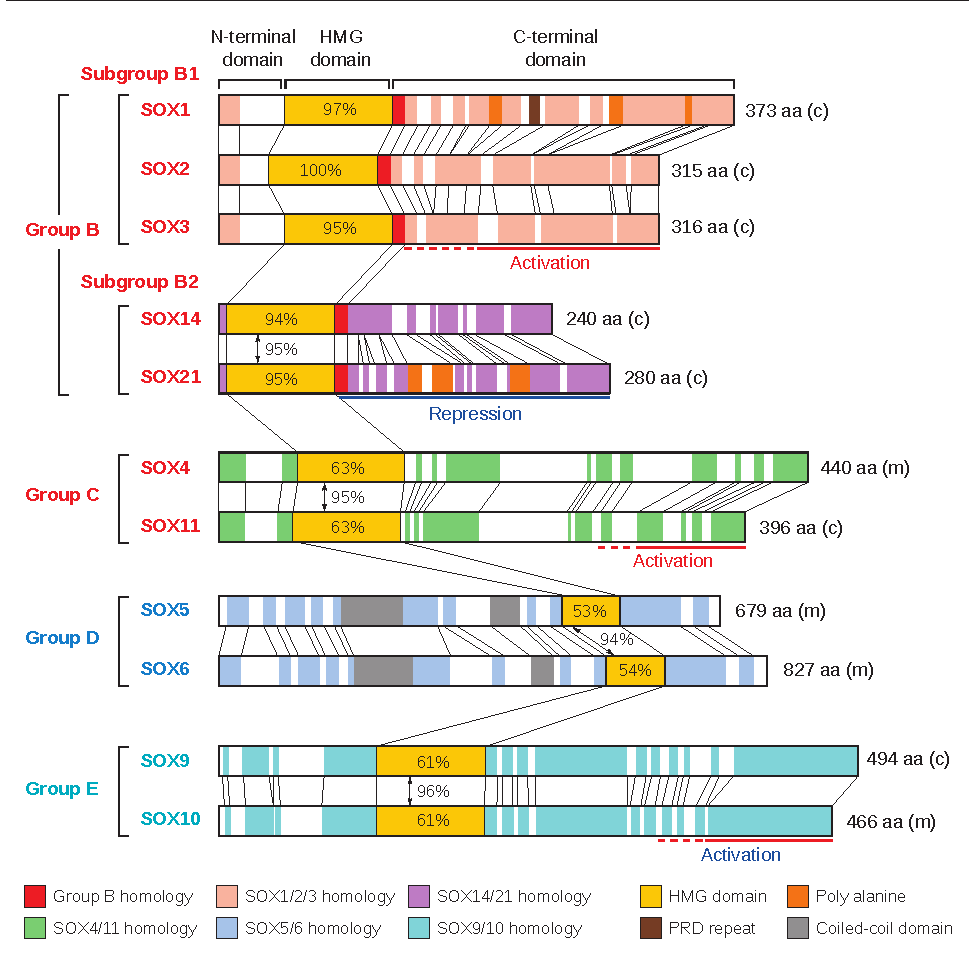
\includegraphics[width=\textwidth]{figs/Fig1 Kamachi et al.pdf}
\label{fig1}
\caption{\textbf{Diversity in Sox protein sequence homology.} Reprinted with permission from Kamachi \emph{et al.} \protect\citeyear{kamachi_pairing_2000}.  Representative mammalian members of Sox families B through E are shown with sequence homology within the HMG domain quantified in comparison to Sox2. The HMG domain is the only domain that displays sequence homology between different families. However, there are several other domains that provide sequence homology within a given group; for instance, SoxB1 and SoxB2 genes contain a homology domain specific to group B, and additionally contain homology in activation or repression domains specific to their subgroup.}
\end{figure}

The sole member of the SoxA family is the mammalian testis determining
factor \emph{SRY}, which was the first characterised Sox gene. SoxB
genes are expressed in neural progenitor cells (\gls{NPCs}) and are involved
in maintaining stem cell pluripotency \shortcite{sarkar_sox_2013}.
They also play a vital role in embryogenesis and the formation of the
nervous system \shortcite{guth_having_2008}. This subfamily includes both
\emph{SoxN} and \emph{D} in \emph{Drosophila}, as well as the homologous
\emph{Sox1, 2 and 3} in mice and humans \shortcite{schepers_twenty_2002}. SoxC
genes \emph{Sox4, Sox11,} and \emph{Sox12} are expressed in stem cells
and contribute to differentiation, giving rise to components of the
skeletal, cardiovascular, nervous, and endocrine systems \shortcite{lefebvre_soxc_2016}. As with the SoxB family, SoxD is also involved in
neurodevelopment and embryogenesis, and its member \emph{Sox6} is a
downstream regulatory target of Sox2 \shortcite{ji_soxd_2016}. Despite not
containing transactivation or transrepression domains, they are known to
perform transcriptional activation and repression and play a role in
both lymphocyte differentiation and erythropoiesis \shortcite{chew_yin_2009,lefebvre_soxd_2010}. SoxE is implicated in a variety of stem cell related
functions, and lineage tracing experiments have shown that Sox9 plays a
broad role in priming progenitor cells for differentiation in
intestinal, hepatic, pancreatic, mammary, and retinal tissues \shortcite{furuyama_continuous_2011,sarkar_sox_2013}. Sox9 also acts downstream
of SRY together with SoxE members Sox8 and Sox10 as well as with SoxB
member Sox3 to regulate the development of gonadal cells during sex
differentiation \shortcite{graves_interactions_1998, she_sry_2017}. The SoxF family plays
a vital role in developing both the cardiovascular and lymphatic
systems, and mutations in the SoxF gene \emph{Sox18} are associated with
hypotrichosis--lymphedema--telangiectasia syndrome (\gls{HLTS}), a lymphatic
disorder \shortcite{francois_soxf_2010,hokari_changes_2008}. Evidently, Sox
transcription factors provide a diverse arsenal of developmental and
regulatory controls that are conserved between animal species. The
several subfamilies represent structural similarities that translate
into broad functional redundancy and conservation.

Much of the specificity and diversity of Sox genes comes from their
partner factors. Early studies into the expression of the Sox2 target
gene Fibroblast Growth Factor 4 (\emph{FGF-4}) showed that neither Sox2
nor its cofactor Oct-3 were alone sufficient to induce \emph{FGF-4}
expression, but together, the Sox2/Oct-3 complex could interact with the
protein Oct-1 to bind the \emph{FGF-4} enhancer and drive expression
\shortcite{yuan_developmental-specific_1995}. These Oct proteins bind preferentially to specific
DNA octomer motifs, and are a subfamily of POU homeodomain TFs known to
be common cofactors of Sox TFs \shortcite{tantin_oct_2013}. Because both Sox and Oct
TFs have their own sequence-specific binding profiles, specific Sox and
Oct gene combinations can result in complexes that can target enhancer
sequences of a relatively small subset of genes at a time, lending
tissue specificity to the Sox-partner code \shortcite{kondoh_soxpartner_2010}.

One of the most well-studied examples of these Sox-partner interactions
is the interplay between Sox2 and Oct-3/4. When both are coexpressed,
the resulting complex can drive expression not only of target genes that
define the embryonic stem cell (\gls{ES cell}) state, but also for the \emph{Sox2}
and \emph{Oct-4} genes themselves, allowing the complex to stabilise its
own expression and cell type \shortcite{kamachi_sox_2013,kondoh_interplay_2004}. Interestingly, more recent work has shown that in the context of
ES and neural progenitor cells, Sox2 acts as a pioneer factor to open
chromatin and facilitate POU binding \shortcite{mistri_selective_2015}. There is
evidence that the Sox-POU interaction is conserved since, as described
below, Dichaete is known to interact with the POU protein Ventral veins
lacking in the CNS midline \shortcite{soriano_drosophila_1998}.

In addition to stabilising an existing cell type, Sox-partner
interactions can also drive the transition to the next stage of
development. A Sox-partner complex is capable of driving expression of
another TF that can then complex with either the original Sox gene or
its cofactor to promote the expression of genes for a new stage of
development \shortcite{kamachi_sox_2013}. This is the case when Sox10 and
its cofactor Pax3 promote expression of the \emph{Mitf} gene, encoding a
TF that partners with Sox10 to drive genes that differentiate neural
crest cells into melanocytes \shortcite{bondurand_interaction_2000,ludwig_melanocyte-specific_2004}. Modern sequencing techniques have provided a quantitative look at
the interaction profiles of Sox TFs and their POU-domain cofactors,
revealing that Sox2 is capable of cooperating not only with Oct-3/4 but
also with several of the class III POU factors that are endogenously
coexpressed with Sox2 in neural cells \shortcite{chang_quantitative_2017}.
Heterodimerisation is not the only mode that Sox TFs can use, as SoxD
and SoxE proteins have been found to homodimerise and act as their own
cofactors \shortcite{lefebvre_control_2007}. Thus, the Sox-partner code can either
stabilise a cell type or drive subsequent stages of tissue
differentiation. Sequence-level specificity of Sox genes and their
binding partners allows them to target specific subsets of genes in
different cell types, and the interplay between these factors can both
maintain and progress developmental stages. These processes exemplify
the regulatory versatility of Sox genes at the molecular level.

\subsection{SoxB subfamily}

Of the Sox subfamilies, the SoxB group is particularly relevant for
understanding and modelling animal development. This group contains the
mammalian gene \emph{Sox2}, which, as mentioned previously, has diverse
roles related to ES cell pluripotency, and neural development. Many of
the functions mediated by Sox2 depend on expression of specific
cofactors, conferring a tissue specificity to its TF activity. For
instance, interaction with Oct-3/4 will drive genes necessary for ES
cell pluripotency, while interaction with the TF Pax6 drives the
expression of crystallin to promote induction of the eye lens \shortcite{bernard_acquisition_2010,kamachi_pax6_2001,kondoh_interplay_2004}.
Antagonistic interactions between Sox2 and tissue-specific cofactors
occur in a dosage-dependent manner to regulate cell fate in the
neuroectoderm, digestive system, and peripheral nervous system, among
others \shortcite{sarkar_sox_2013}. While \emph{Sox2} is one of the
most well-studied Sox genes in vertebrates, it is far from the only
major player in the SoxB subfamily.

The SoxB group is divided into subgroup SoxB1 (Sox1, 2 and 3), which
generally comprises transcriptional activators, and SoxB2 (Sox14 and
21), which are generally transcriptional repressors \shortcite{uchikawa_two_1999}. These subfamilies interplay in vertebrates to regulate neural
formation. This requires a balancing act between Sox1-3, which keep stem
cells in a pluripotent state, and Sox21, which commits them to
differentiation \shortcite{sandberg_sox21_2005,wegner_all_2010}. In
\emph{Drosophila}, sequence based analysis indicates that the SoxB1
group contains \emph{SoxN} \shortcite{kamachi_sox_2013,phochanukul_no_2010}. The SoxB2 subgroup in \emph{Drosophila} contains
\emph{Dichaete}, \emph{Sox21a,} and \emph{Sox21b} \shortcite{cremazy_genome-wide_2001,nambu_drosophila_1996,russell_dichaete_1996,uchikawa_two_1999}.
However, sequence homology analysis appears to show that \emph{Sox21a}
is closer to vertebrate subgroup B2 while \emph{Sox21b} and \emph{D} are
more likely to represent an invertebrate-specific SoxB subgroup
\shortcite{mckimmie_conserved_2005}.

Compared to \emph{SoxN} and \emph{D}, the fly genes \emph{Sox21a} and
\emph{Sox21b} are less well-characterised. However, \emph{Sox21a} has
been studied in the context of intestinal stem cells (\gls{ISCs}). Unlike many
other SoxB members, \emph{Sox21a} appears to function primarily in adult
flies and its mutants show no defects during development, although it is
expressed in the embryo gut anlage \shortcite{mckimmie_conserved_2005,meng_sox_2015}. There is less known about the role of \emph{Sox21b}, but
it has been found to localise to the embryonic hindgut \shortcite{cremazy_genome-wide_2001,mckimmie_conserved_2005}. In wild type flies, \emph{Sox21a} acts as
a tumor suppressor and helps ISCs transition from enteroblasts to
enterocytes \shortcite{meng_sox_2015,zhai_accumulation_2015}; when faced with
cellular damage resulting in oxidative stress, \emph{Sox21a} expression
decreases and results in a feedback loop that proliferates
differentiation-defective enteroblasts that help with tissue repair \shortcite{chen_feedback_2016}. Its proliferative and regenerative properties come
as a result of being downstream of the JNK, ERK, and JAK/STAT pathways
\shortcite{meng_sox_2015,zhai_genetic_2017}, and DamID experiments suggest
that it may join as a cofactor with the repressive TF Capicua (Cic) in
ISCs and enteroblasts to control differentiation downstream of the EGF
pathway \shortcite{doupe_drosophila_2018}. While less is known about \emph{Sox21b},
sequence analysis has shown that both \emph{Sox21a} and \emph{Sox21b}
contain introns in their HMG box, and that a conserved genomic cluster
of \emph{D}, \emph{D} 3' regulatory sequences, \emph{Sox21b}, and
\emph{Sox21a} \shortcite{mckimmie_conserved_2005,wilson_evolution_2008} appears in several analysed insect species (Figure 2). This points to
a model in which these three genes, as well as \emph{SoxN}, may have
evolved as a result of redundant duplication and specialisation of an ancestral SoxB gene.

\setcounter{figure}{2-1}
\begin{figure}[htbp]
\centering
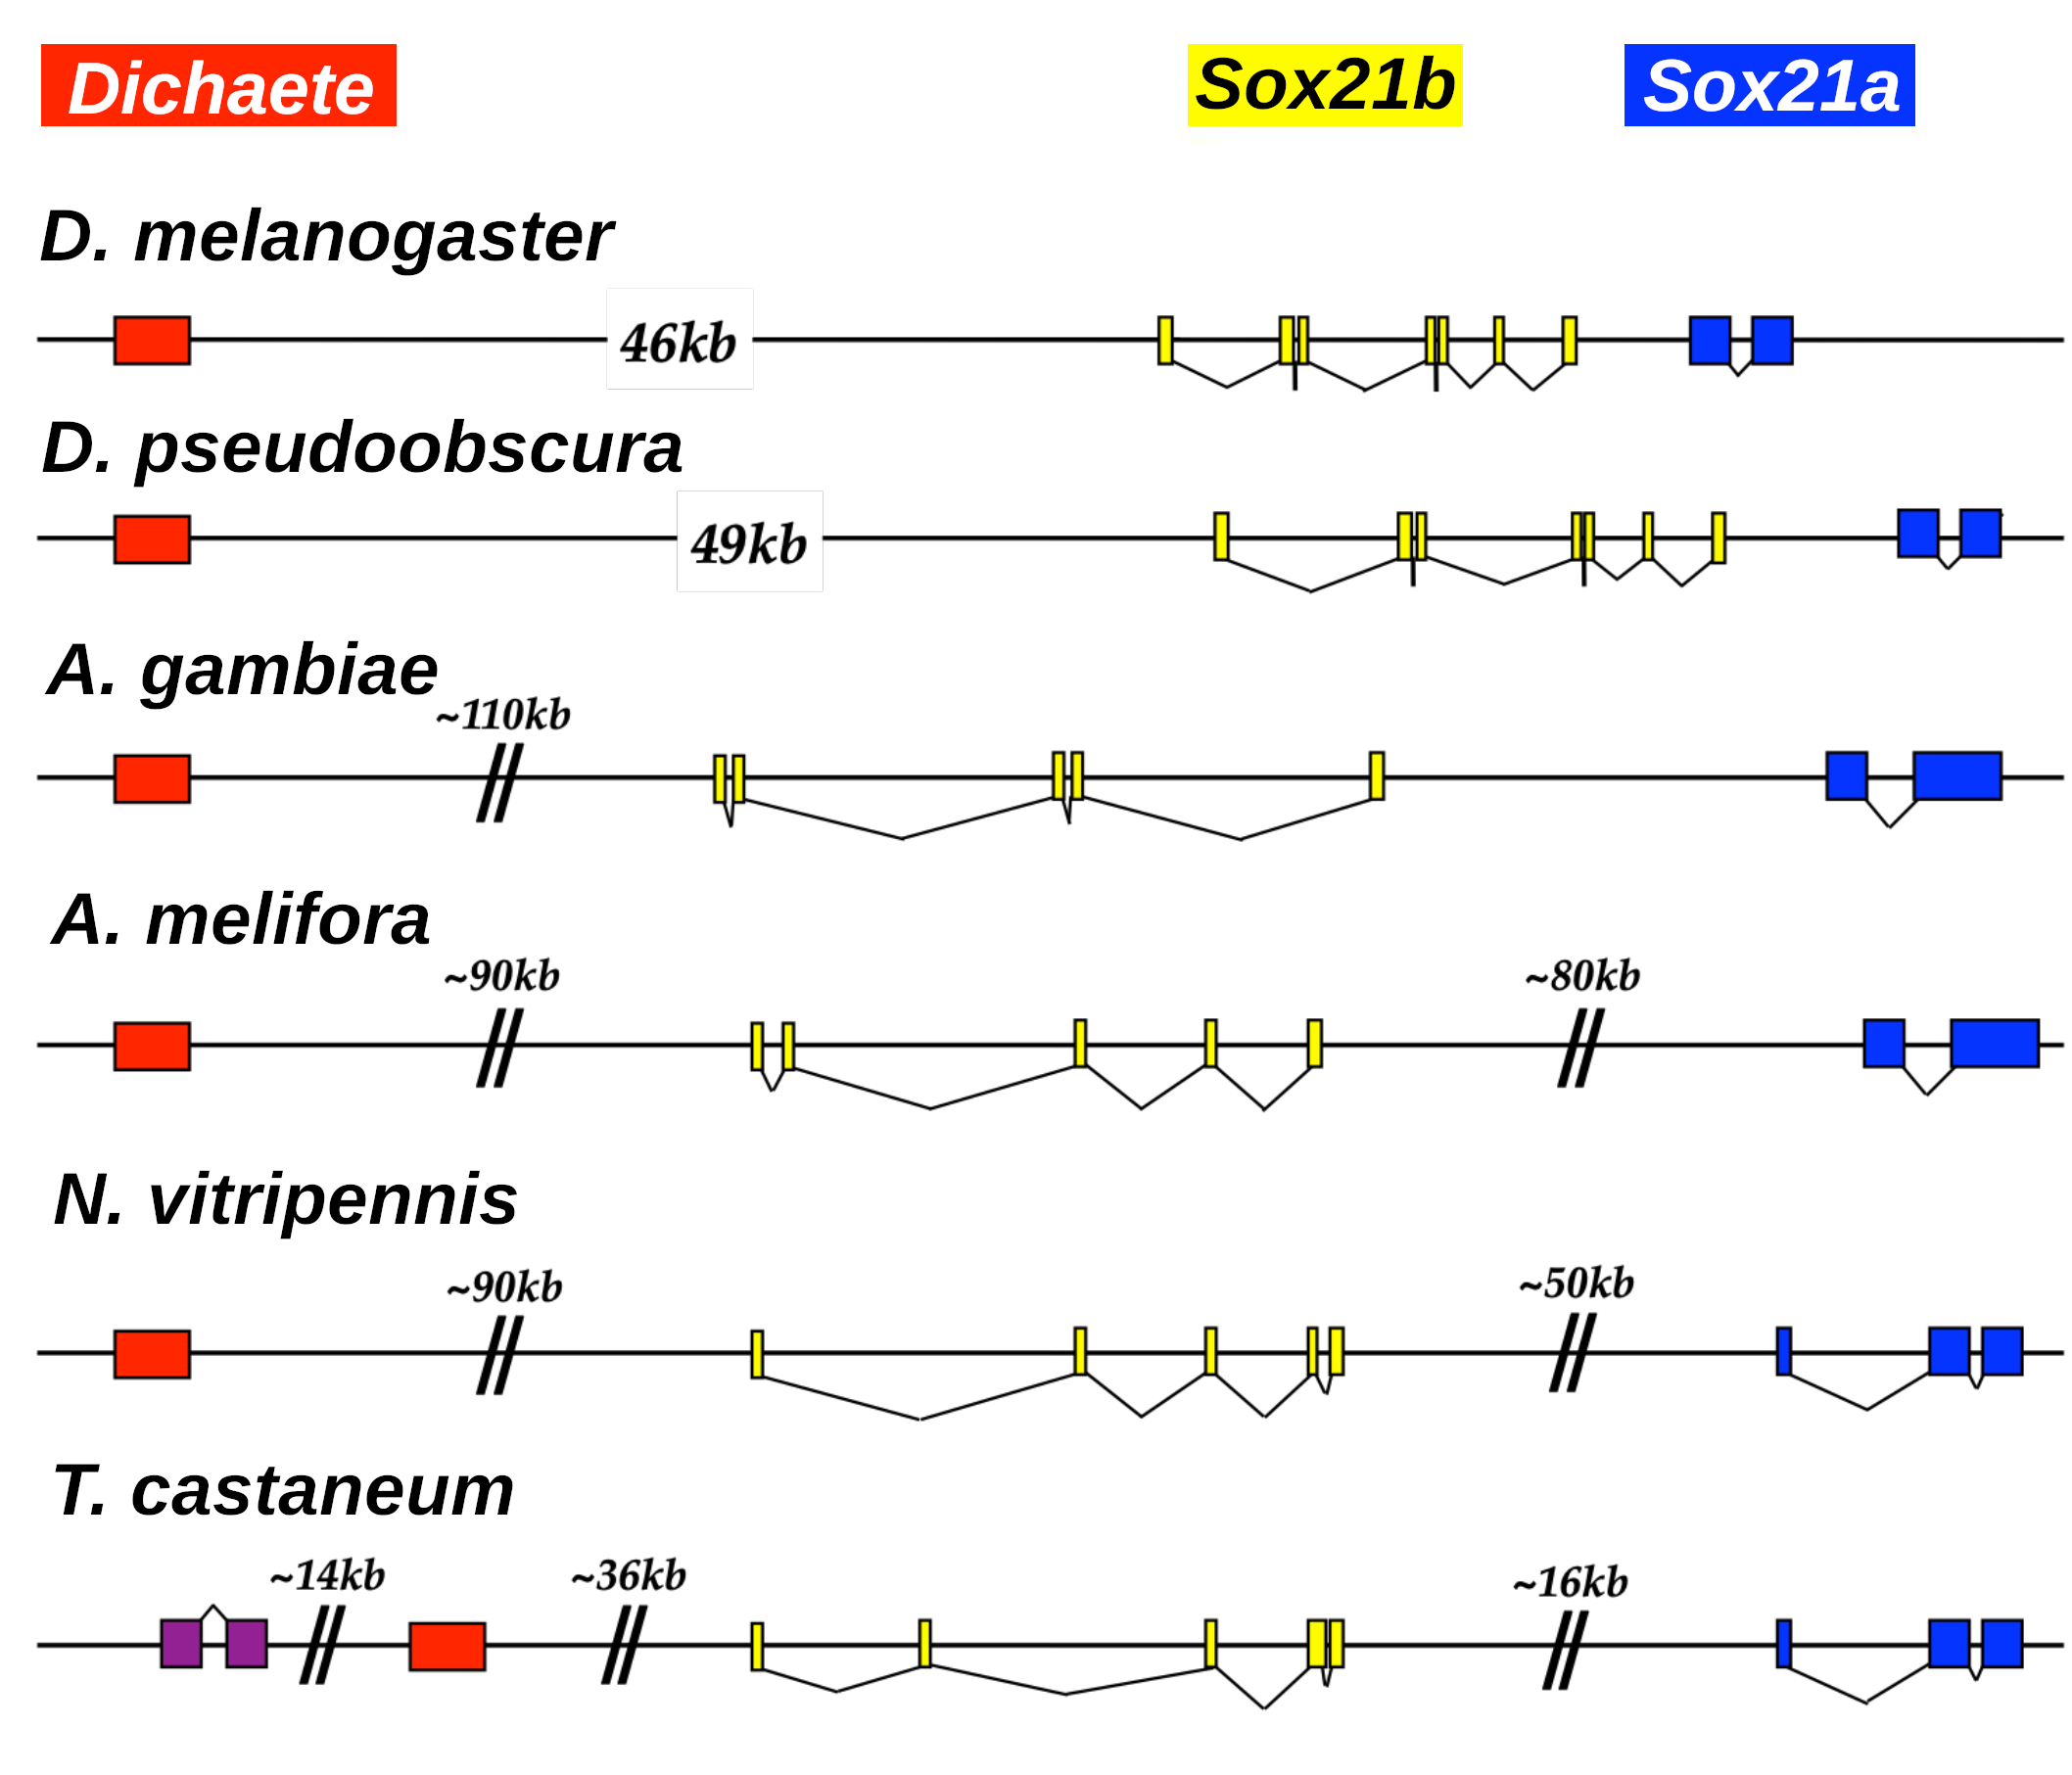
\includegraphics[width=.8\textwidth]{figs/Figure 2 D_Cluster.png}
\label{fig2}
\caption{\textbf{Conserved cluster of \emph{Dichaete}, \emph{Sox21b}, and \emph{Sox21a}.} The cluster of \emph{D}, \emph{Sox21b}, and \emph{Sox21a} is conserved in several analysed insect species including the \emph{Drosophila} species \emph{melanogaster} and \emph{pseudoobscura}, the mosquito \emph{A. gambiae}, the honeybee \emph{A. melifora}, the wasp \emph{N. vitripennis}, and the beetle \emph{T. castaneum}.  Data adapted from McKimmie \emph{et al.} \protect\citeyear{mckimmie_conserved_2005} and Wilson \& Dearden \protect\citeyear{wilson_evolution_2008}. Modified from figure provided by S. Russell (personal communication, 28 Aug 2020).}
\end{figure}

While Sox B1 and B2 genes in vertebrates exhibit a relatively pronounced
distinction between activation and repression, the respective
\emph{Drosophila} genes \emph{SoxN} and \emph{D} exhibit much more
overlap in terms of function, localisation, and regulatory control
\shortcite{neriec_different_2014}. As a result, it is difficult to characterise
either of them as directly homologous to any particular vertebrate SoxB
gene, although given the functional arguments below, it is likely that
SoxN is a true orthologue of the SoxB1 family. In common with the
vertebrate SoxB1 family, SoxN and D show a degree of functional
redundancy which is of some interest, as identifying the shared and
unique properties of the two genes can elucidate much of the behavior of
SoxB TFs in animal systems. Interestingly, \emph{SoxN} and \emph{D} are
known to be intronless in insects and vertebrate SoxB1 genes have been
confirmed to be intronless in humans, mice, and chickens \shortcite{mckimmie_conserved_2005,uchikawa_two_1999}. Because \emph{Drosophila} genes
often contain regulatory sequences in their first intron \shortcite{marais_intron_2005}, these genes represent a subset of Sox factors that can be swapped
into the endogenous \emph{SoxN} or \emph{D} loci without introducing
secondary regulatory effects. This primes \emph{Drosophila} as a useful
system for studying the effects of introducing exogenous SoxB genes to
the fly genome.

Both \emph{SoxN} and \emph{D} are expressed in the neuroectoderm of the
developing \emph{Drosophila} embryo, where they overlap in the medial
and intermediate columns. In addition, \emph{D} is expressed in the
ventral midline from its formation, while \emph{SoxN} shows expression
in the lateral column of the neuroectoderm where \emph{D} is absent
\shortcite{cremazy_sox_2000,phochanukul_no_2010}. This tissue
specificity supports functional differences between the two genes during
development, as \emph{D} is necessary for proper midline formation
\shortcite{soriano_drosophila_1998} while SoxN is necessary for lateral
neuroblast differentiation \shortcite{overton_evidence_2002}. In the medial and
intermediate neuroectoderm where both genes are expressed, single
mutants for either gene display only mild Central Nervous System (\gls{CNS})
phenotypes, but double mutants show severe neural hypoplasia \shortcite{buescher_formation_2002,overton_evidence_2002}, suggesting that these genes can
partially compensate for each other in the tissues where they are
coexpressed.

The functional differences between SoxN and D may be better understood
through their DNA binding profiles. DNA adenine methyltransferase
identification (DamID) and ChIP experiments have shown both TFs binding
to 1,890 common genes, with S\emph{oxN} uniquely binding to 1,649 genes
and \emph{D} uniquely binding to 1,753 \shortcite{ferrero_soxneuro_2014}. In
mutants that were null for either gene, DamID using the remaining TF
showed that both \emph{SoxN} and \emph{D} were able to bind some of the
missing TF's unique targets, indicating functional compensation at the
genomic level. However, this was not the only behavior exhibited, as
some regions demonstrated \emph{de novo} binding of the remaining TF
\shortcite{ferrero_soxneuro_2014}. This illustrates that on the level of molecular
binding, the partial redundancy lets either TF rescue some of the
other's function, but also causes behavior that deviates from the wild
type. Later experiments showed not only that \emph{SoxN} and \emph{D}
share common binding targets in \emph{Drosophila melanogaster}, but that
genes targeted by both TFs were more likely to display binding
conservation in \emph{Drosophila simulans}, suggesting conservation not
only of the TFs themselves but also of their regulatory networks \shortcite{carl_common_2015}. While \emph{SoxN} and \emph{D} share several
similarities, it is also informative to examine the areas in which they
are unique. Their differences represent clues to their non-redundant
functions in \emph{Drosophila}, and many of their unique functions are
preserved in related species.

The \emph{Dichaete} gene was independently identified by two different
groups who noted its unique role in embryonic segmentation. Russell
\emph{et al.} showed that the HMG gene known as \emph{Sox70D}
corresponded to the known mutation \emph{Dichaete} and then demonstrated
that it is necessary in early embryogenesis for normal segmentation
where it regulates the pair-rule segmentation genes \emph{even-skipped},
\emph{hairy}, and \emph{runt} \shortcite{russell_dichaete_1996}. Simultaneously,
Nambu \& Nambu identified the gene as \emph{fish-hook} (\emph{fish})
based on its expression pattern in the embryo and identified similar
segmentation defects in mutants, also suggesting roles in CNS
development \shortcite{nambu_drosophila_1996}. Assays based on lacZ reporters
showed that the sequences flanking \emph{D} contain multiple enhancer
elements that determine its complex expression across embryogenesis, and
identified functions in hindgut development, in \emph{hedgehog}
(\emph{hh}) and \emph{decapentaplegic} (\emph{dpp}) signalling, and in
brain development \shortcite{sanchez-soriano_regulatory_2000}.

Later work showed that \emph{D} also plays a role in CNS patterning
along the dorsoventral (\gls{DV}) axis and that it works downstream of
\emph{Epidermal growth factor receptor} (\emph{Egfr}) and in concert
with both \emph{intermediate neuroblasts defective} (i\emph{nd}) and
\emph{ventral nerve cord defective} (\emph{vnd}) to determine the
cellular fate of neuroblasts at different parts of the DV axis \shortcite{zhao_sox-domain_2002}. Work in the CNS established not only that \emph{D} was
expressed in the CNS midline, but also that it was necessary for proper
midline formation \shortcite{soriano_drosophila_1998}. In this role D forms
complexes with Single minded and the POU domain protein Ventral veins
lacking to regulate the expression of \emph{Slit}, a midline-expressed
gene responsible for normal axon formation at the midline \shortcite{ma_functional_2000}. Of interest, these studies also showed that Sox2 could
functionally substitute for Dichaete in the midline. Screens with
dominant-negative variants of \emph{D} identified \emph{commisureless}
(\emph{comm}) and \emph{asense} (\emph{ase}) as direct targets, and also
found other targets specific to tissue type and developmental stage
\shortcite{shen_identifying_2013}. ChIP-array and \gls{DamID} binding data along with gene
expression data identified \emph{D} as a regulatory hub during
embryogenesis, with many of its direct targets serving also as conserved
targets for the related TF \emph{Sox2} in mammals \shortcite{aleksic_role_2013}. These experiments highlight the diversity of the known functions
performed by \emph{Dichaete}, ranging from developmental regulation of
segmentation to promotion of neurodevelopment. In particular, the unique
segmentation and axis patterning phenotypes of \emph{Dichaete} and its
close homologues appear to be conserved in other arthropod species, even
though they do not share the exact same expression patterns as in
\emph{Drosophila} \shortcite{clark_evidence_2018,phochanukul_no_2010,paese_soxb_2018}.

In contrast, the functions of \emph{SoxN} appear much more specific to
CNS development. \emph{SoxN} was first identified as part of a PCR
screen of embryonic cDNA, and its expression was found to be under the
control of zygotic DV patterning genes such as \emph{dpp} and
\emph{twi}, linking its expression to the patterning established by
\emph{D} \shortcite{cremazy_sox_2000}. SoxN expression was found to colocalise
with D expression in the CNS and PNS, with unique expression in the
lateral column and no expression in the midline \shortcite{cremazy_sox_2000,phochanukul_no_2010}. \emph{SoxN} was found to be necessary for
neuroblast formation, with mutants defective in the lateral column of
the neuroectoderm where \emph{D} is unable to compensate for its loss;
this phenotype was more pronounced in mutants also lacking \emph{vnd} or
\emph{ind}, suggesting that these TFs interact with both SoxN and D to
give rise to ventral and intermediate neuroblast formation \shortcite{buescher_formation_2002,overton_evidence_2002,zhao_sox-domain_2002}. The complexities
of these interactions were further explored in the context of ubiquitous
ectopic \emph{Egfr} expression, which caused \emph{vnd} and \emph{ind}
to be expressed more in the lateral neuroectoderm where they could then
act as \emph{SoxN} cofactors; this suggests both spatial and temporal
regulation of \emph{vnd} and \emph{ind} by \emph{Egfr} in wild-type
neuroblast development \shortcite{zhao_genetic_2007}. The neuroblast formation
phenotype of \emph{SoxN} was also found to work upstream and in parallel
with the proneural \emph{achaete/scute} gene complex (\emph{\gls{AS-C}})
genes, with both \emph{SoxN} and the \emph{AS-C} members \emph{achaete}
(\emph{ac}), \emph{scute} (\emph{sc}), and \emph{lethal of scute}
(\emph{l'sc}) contributing to neuroblast formation through separate
mechanisms \shortcite{buescher_formation_2002,overton_evidence_2002}. Thus, several
of the major proneural genes involved with segment patterning
\shortcite{hartenstein_initial_2013} have interactions with both \emph{SoxN}
and \emph{D} during the course of neurogenesis.

Later work highlighted the role of \emph{SoxN} in signalling pathways
such as Wg/Wnt, where it was shown to act as a negative regulator of
\emph{wingless} (\emph{wg}) activity in flies through interaction with
the HMG-containing TF Pangolin (Lef/Tcf) \shortcite{chao_hmg-box_2007}.
\emph{SoxN} was found to work in concert with \emph{D} and
antagonistically with \emph{wg} to activate \emph{shavenbaby}
(\emph{svb}), leading to the formation of trichome projections in the
epidermis \shortcite{overton_drosophila_2007}. This indicates the possible relevance
of \emph{SoxN} and its homologues to canonical vertebrate and
invertebrate signalling pathways. While its functions in early CNS
development exhibit conservation in other species, several of its
functions later in development appear unique to \emph{Drosophila},
suggesting a model in which \emph{SoxN} evolved from an ancestral
metazoan SoxB and kept its basic functions while also undergoing
additional functional specialisation specific to flies \shortcite{ferrero_soxneuro_2014}. Altogether, these studies point to ways in which \emph{SoxN} and
\emph{D}, despite their unique expression patterns and functions, help
regulate some of the same systems during development.

\section{Evolution and specification of SoxB genes}

Sox genes in different animal species exhibit a high degree of
structural and functional similarities, but also exhibit unique
species-specific functions. Given the relative functional conservation
of its broad subfamilies across species, this raises the question of how
Sox genes in their current form originated and how they gained their own
specialised functions. Evidence points to an evolutionary history of Sox
genes in the animal kingdom in which Sox genes originated from
duplication of an ancestral HMG gene in metazoa or choanozoa \shortcite{jager_expansion_2006}, suggesting that diversification of the Sox gene family
occurred prior to the formation of the Bilateria clade that contains
both arthropods and chordates. Within the animal kingdom, there has been
a stable core set of Sox genes in subfamilies B through F, indicating
that the last common ancestor (\gls{LCA}) of chordates contained this core set
in addition to a SoxH gene \shortcite{heenan_evolution_2016}, whereas the arthropods
inherited only the core set of genes.

Specifically for SoxB genes, phylogenetic reconstruction based on
sequence alignment of HMG domain genes has suggested that the bilaterian
LCA contained a SoxB1 gene and a SoxB2 gene, and that both of these
genes followed separate evolutionary paths following the divergence of
arthropods from chordates \shortcite{zhong_parallel_2011}. Prior models had
suggested that SoxB genes diversified through separate genome
duplication and tandem duplication events following the
deuterostome/protostome split \shortcite{mckimmie_conserved_2005}, but the presence
of SoxB1 and SoxB2 in the bilaterian LCA suggests that a tandem
duplication event occurred prior to the split \shortcite{zhong_parallel_2011}. In
humans, it is suggested that \emph{Sox1-3} evolved from genome
duplication events affecting the \emph{SoxB1} copy, while \emph{Sox14}
and \emph{Sox21} arose from genome duplications of the \emph{SoxB2}.
Meanwhile, in insects, the model suggests that \emph{SoxB2} underwent
two tandem duplications to give rise to \emph{Sox21a}, \emph{Sox21b},
and \emph{Dichaete}, and that \emph{SoxB1} specialised to give rise to
\emph{SoxNeuro} (Figure 3) \shortcite{zhong_parallel_2011}. This explains the
presence of the conserved cluster of \emph{D-Sox21a-Sox21b} and their
related enhancer sequences present in all sequenced insect species to
date \shortcite{mckimmie_conserved_2005,paese_soxb_2018,phochanukul_no_2010}.

\setcounter{figure}{3-1}
\begin{figure}[htb]
\centering
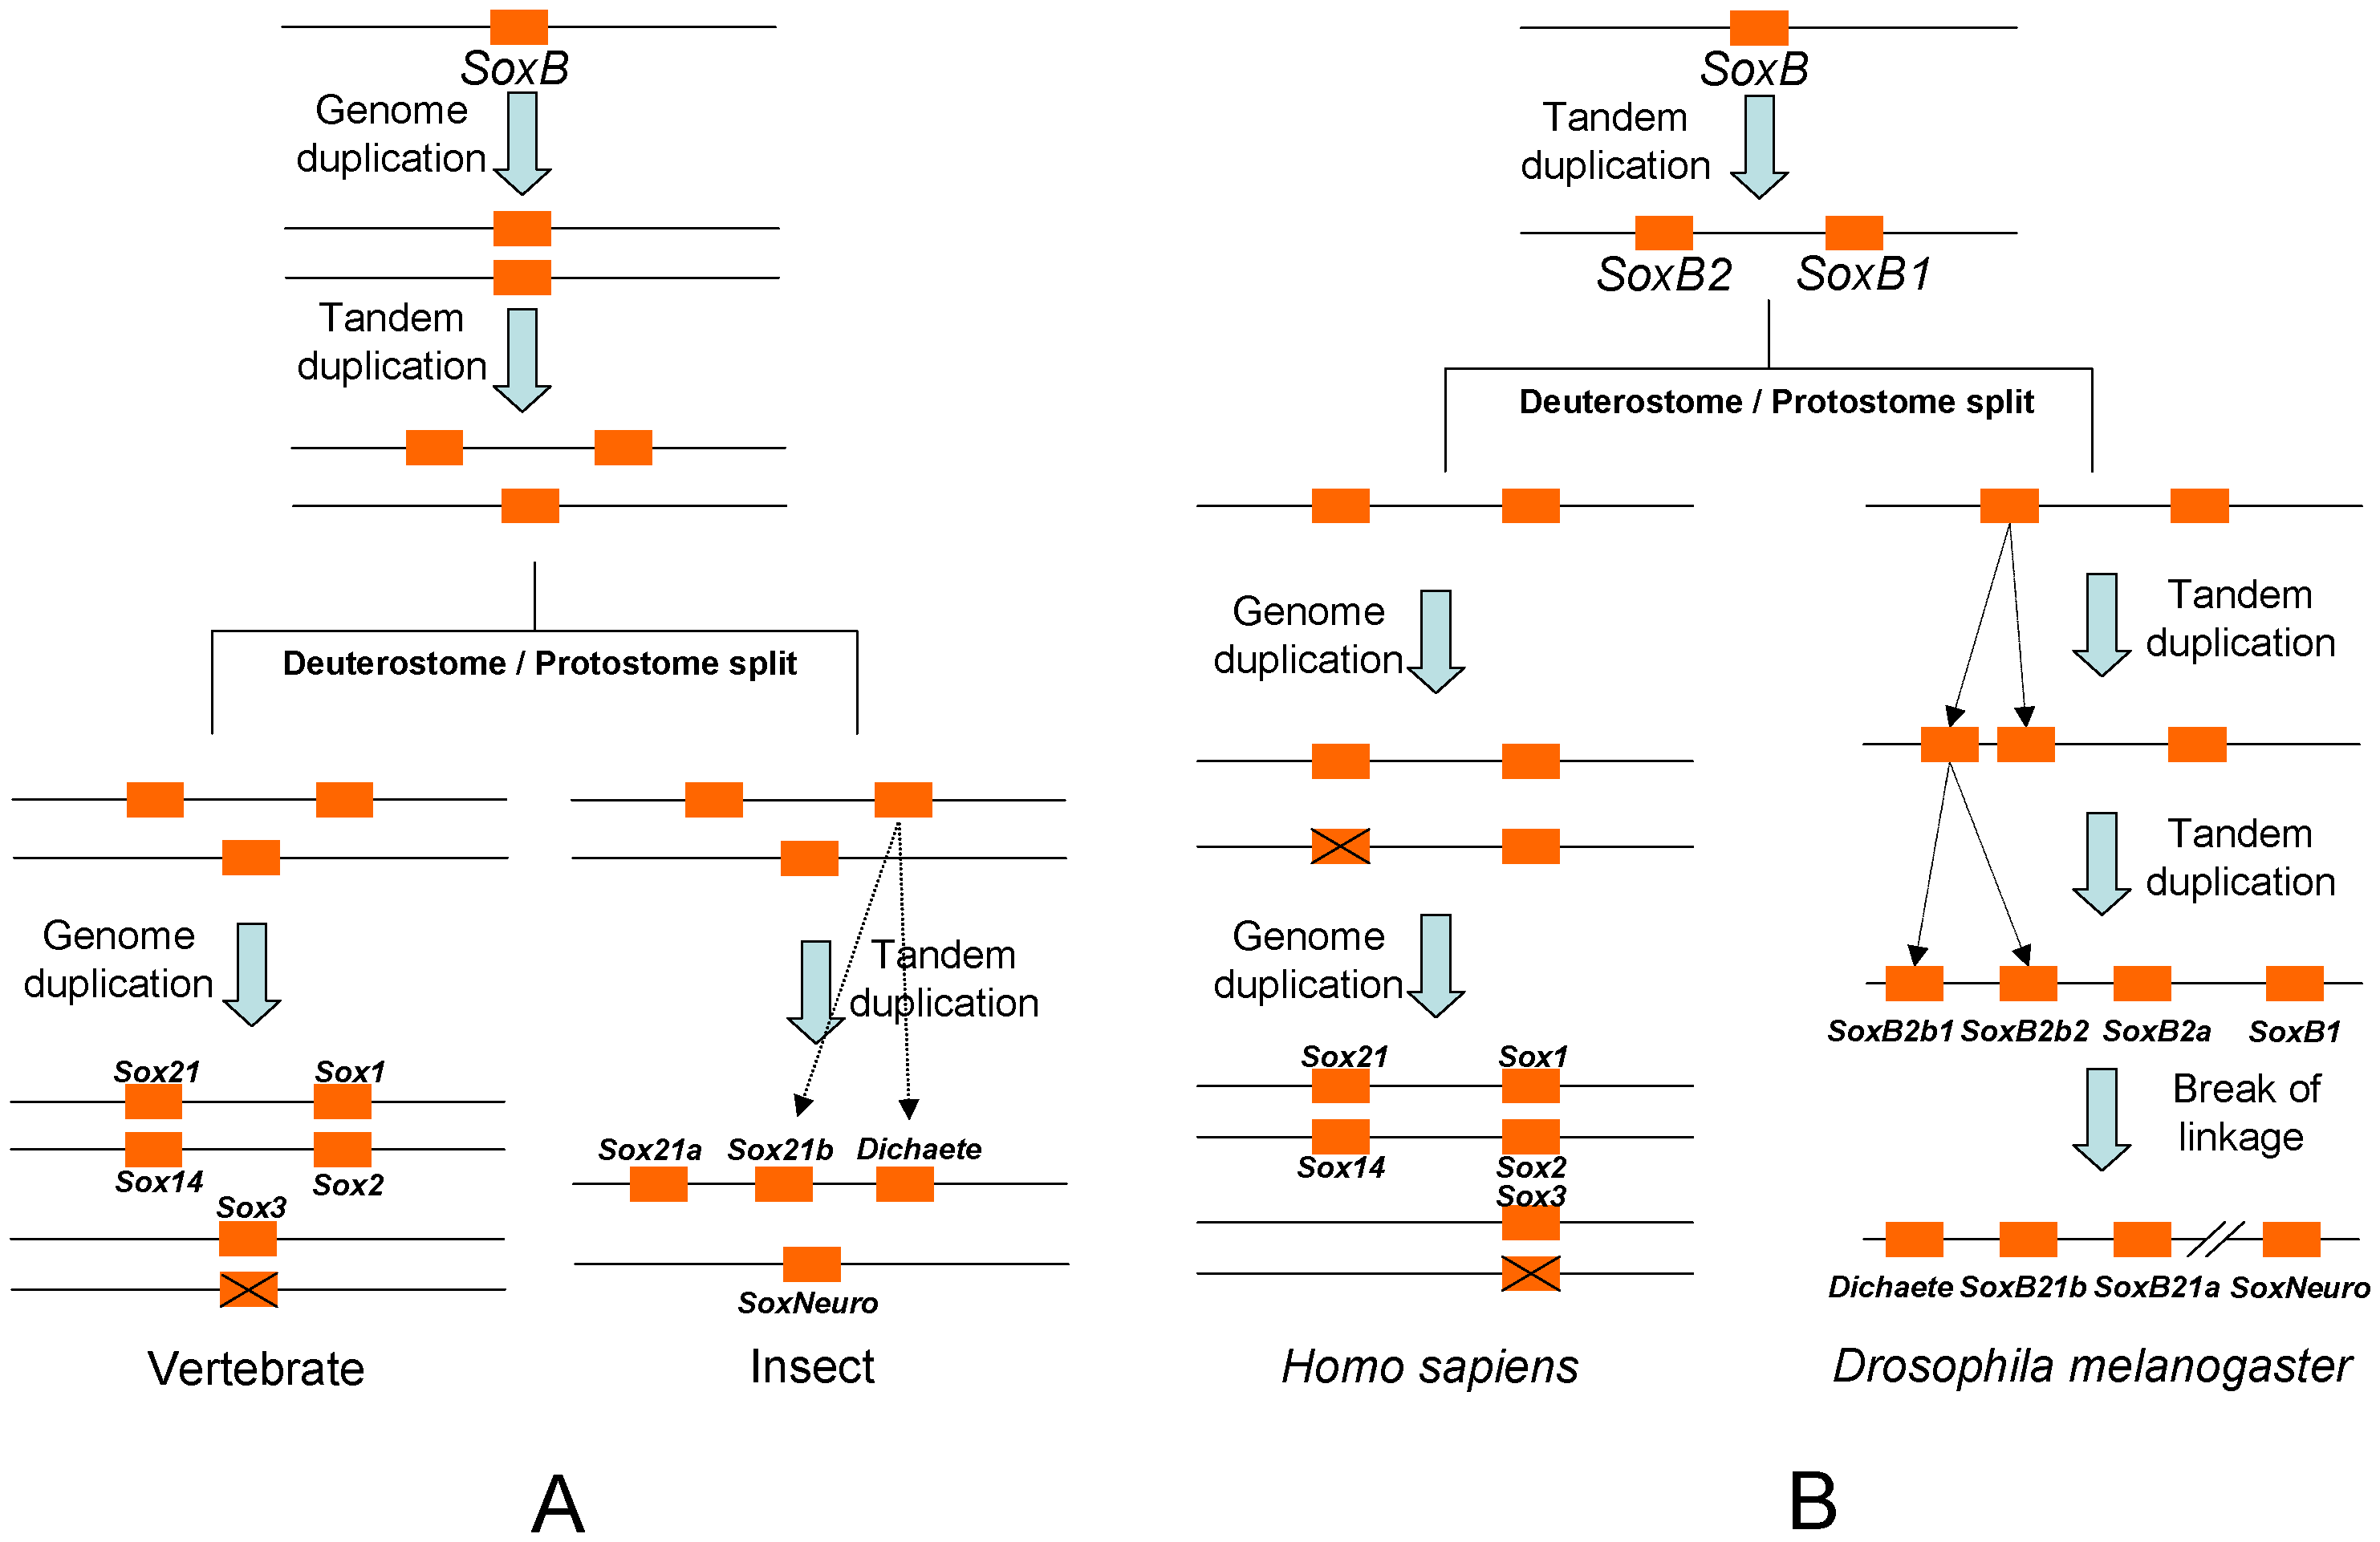
\includegraphics[width=\textwidth]{figs/Figure 3 Zhong vs McKimmie.png}
\label{fig3}
\caption{\textbf{Models for SoxB evolutionary history.} The diversity in \emph{SoxB} genes was attributed to both tandem duplications and genome duplications. \textbf{(A)} McKimmie \emph{et al.} \protect\citeyear{mckimmie_conserved_2005} proposed that \emph{SoxN} and \emph{D} diverged due to an ancestral genome duplication, followed by a tandem duplication that gave rise to \emph{Sox21a} and an insect-specific tandem duplication that resulted in \emph{Sox21b}. \textbf{(B)} However, Zhong \emph{et al.} note that the bilaterian LCA possessed both \emph{SoxB1} and \emph{SoxB2}, suggesting that an ancestral tandem duplication occurred first; further tandem duplications gave rise to the conserved cluster in insects while genome duplications and pseudogenisation contributed to the current vertebrate \emph{SoxB} organisation. Reprinted from Zhong \emph{et al} \protect\citeyear{zhong_parallel_2011}.}
\end{figure}

The evolutionary history of SoxB in insects raises the question of
whether there are also functional commonalities between related genes in
different species. Studies comparing Sox proteins in \emph{D.
melanogaster}, \emph{A. gambiae}, the honeybee \emph{Apis mellifera},
the wasp \emph{Nasonia vitripennis}, and the beetle \emph{Tribolium
castaneum} (\gls{Tc}) found that each of these insect groups contain eight or
nine Sox genes in total, with \emph{SoxB} as the largest subgroup with
at least four members per species \shortcite{wilson_evolution_2008}. DamID
binding analysis of \emph{SoxN} and \emph{D} in four \emph{Drosophila}
species reveals that while the common targets of both TFs display some
binding conservation in other species, suggesting functional importance
of the shared targets, binding site turnover as a result of compensatory
evolution is proportional to phylogenetic distance between species and
may account for changes in gene expression as well as function \shortcite{carl_common_2015}.

Tandem duplication and genome duplication events explain why there are
so many \emph{SoxB} genes in insects, but do not on their own explain
their functional similarities and differences. In the case of
neofunctionalisation, SoxB genes would be expected to show changes in
their coding sequence or their flanking regulatory sequences. However,
it is known that the \emph{SoxB2} sequence cluster in \emph{Drosophila}
is highly conserved across the insects \shortcite{mckimmie_conserved_2005}. The
shared regulatory controls therefore point to a model in which SoxB
factors share a network of conserved gene targets to maintain the
robustness of SoxB downstream regulation while individual SoxB members
can pick up different targets to specialise their expression and
targeting spatially and temporally \shortcite{carl_common_2015,neriec_different_2014}. In other words, SoxB genes can maintain a shared
regulatory network of conserved targets from the ancestral gene \shortcite{aleksic_role_2013,ferrero_soxneuro_2014,neriec_different_2014} while
evolutionary distance from related species can allow them to pick up new
expression patterns and functions \shortcite{carl_common_2015}.

\subsection{Conservation in invertebrates}

Because the evolutionary history of Sox genes caused an expansion of
similar SoxB genes in arthropod species, it is important to examine how
arthropod SoxB expression is both similar and different to the
\emph{Drosophila} model. Namely, \emph{Dichaete} and its close
homologues in different species appear to retain functions related to
segment patterning during embryonic development, while \emph{SoxN} is
expressed in the neuroectoderm in all characterised arthropod species do
date.

\emph{Drosophila} has historically been one of the most versatile
systems for studying segmentation and embryogenesis, but research into
other arthropods reveals ways in which its pathways are not necessarily
representative of invertebrate development. Specific parts of the
developmental cascade differ between species, but the most conserved
components are homologues of \emph{Drosophila} segment polarity genes
\emph{engrailed} (\emph{en}), \emph{wingless} (\emph{wg}), and
\emph{hedgehog} (\emph{hh}) \shortcite{peel_arthropod_2005}. Other parts of the
\emph{Drosophila} system exhibit some partial conservation---each
arthropod contains at least one homologous gene to a \emph{Drosophila}
pair-rule gene \shortcite{peel_arthropod_2005}, but these homologues does not
represent any broadly conserved patterning mechanisms.

Despite significant differences between the \emph{Drosophila} model and
other arthropods, the Sox gene family still has conserved roles relating
to CNS development and segmentation. Janssen \emph{et al.} examined
SoxB-F expression in Tc as well as in the velvet worm
\emph{Euperipatoides kanangrensis} (\gls{Ek}) and the pillbug \emph{Glomeris
marginata} (\gls{Gm}) \shortcite{janssen_embryonic_2018}. They found that \emph{Tc-SoxN}
is expressed in the developing embryonic nervous system, and
\emph{Gm-SoxN} and \emph{Ek-SoxN} are both expressed in the brain and
ventral nervous system. \emph{Tc-}, \emph{Gm-}, and \emph{Ek-Dichaete}
expression varies by species, but shares a common localisation in the
segment addition zone (\gls{SAZ}), where their respective \emph{SoxN} genes
are excluded, and is also expressed in the neuroectoderm. Tc
additionally expresses both \emph{Tc-Sox21a} and \emph{Tc-Sox21b}, with
\emph{Sox21b} largely recapitulating the localisation patterns of
\emph{Dichaete} and \emph{Sox21a} showing much weaker overall
expression. Similar experiments in all three organisms reveal different
localisation patterns in SoxC-F and suggest conserved functional roles
despite their different expression patterns, with SoxC genes taking a
greater role in the developing CNS than in \emph{Drosophila}. Saliently,
the expression of \emph{Dichaete} is related to segmentation in all of
these arthropods, and localisation in the SAZ suggests pair rule
gene-like expression that may be present in the LCA but lost in some
sister clades such as \emph{Apis} \shortcite{janssen_embryonic_2018}.

More practically, \emph{Dichaete} regulation explains how related
processes may govern the development of long germ band and short germ
band insects. While all adult insects share similar body organisation,
the developmental processes they use to pattern the anterior-posterior
(\gls{AP}) axis bear marked differences---long germ band insects like
\emph{Drosophila} pattern all segments of the developing embryo
simultaneously during the blastoderm stage of development, while
intermediate and short germ band insects like \emph{Tribolium} first
specify only anterior segments representing the future head and thorax,
and then extend patterning to the entire embryo by extending at the
posterior segment in a manner akin to vertebrate segmentation \shortcite{liu_short_2005}. Because of the differences in germ band development, the
regulation of these two processes was thought to be substantially
different until Clark \& Peel suggested that a shared cascade of
\emph{Caudal}, \emph{Dichaete}, and \emph{Odd-paired} may explain both
mechanisms \shortcite{clark_evidence_2018}. Spatiotemporal analyses of these three
genes in \emph{Drosophila} and \emph{Tribolium} show that while both
organisms express these factors to regulate pair-rule genes and
influence germ band patterning, \emph{Drosophila} tends to express these
factors as discrete on-off sequential switches while \emph{Tribolium}
expresses them simultaneously but varies their spatial organisation over
time, suggesting \emph{Dichaete} operates within a conserved
developmental framework that differs in regulation rather than substance
\shortcite{clark_evidence_2018}. This result suggests that while arthropods may
share conserved Sox regulatory networks, they can still regulate
expression spatiotemporally to influence the behavior of an individual
Sox factor.

The role of Sox genes has been examined not only in arthropods of the
class Insecta but also in Arachnida. The spiders \emph{Parasteatoda
tepidariorum} (\gls{Pt}) and \emph{Stegodyphus mimosarum} (\gls{Sm}) have both
undergone whole genome duplications during their evolutionary history,
and display higher copy number of genes derived from \emph{Sox21a} and
\emph{Sox21b}, as well as of genes derived from SoxC-F \shortcite{bonatto_paese_duplication_2018}. A spider gene \emph{Sox21b-1} related to \emph{D} and
\emph{Sox21b} is expressed in the SAZ of both Pt and Sm, as was the case
with \emph{Tc-}, \emph{Gm-}, and \emph{Ek-Dichaete}, pointing to a
conserved role that dates back to some arthropod LCA \shortcite{bonatto_paese_duplication_2018,janssen_embryonic_2018}. In Pt, \emph{Dichaete} is not involved
with segmentation, but \emph{Sox21b-1} is known to regulate \emph{fkh}
and \emph{h} in a gap gene-like fashion in the anterior parts of the
embryo as well as \emph{Dl} in the posterior SAZ \shortcite{paese_soxb_2018}.
While \emph{Dichaete} is not specifically involved here, it remains
apparent that \emph{Dichaete}-like genes play a conserved role in
segmentation of arthropods, and that SoxB genes represent a diverse set
of genes with shared regulatory networks and conserved functions.

\subsection{Conservation in vertebrates}

The presence of the SoxA gene \emph{SRY} is a unique but not universal
feature of vertebrates, present in placental and marsupial mammals but
not in their sister monotreme clade, suggesting that \emph{SRY} may
originate in the LCA of eutherians and marsupials \shortcite{katsura_evolutionary_2018,wallis_sex_2007}. PCR-based assays in mice have revealed that
\emph{SRY} is expressed in the urogenital ridge of males but not
females, pointing to the role of \emph{SRY} in testis differentiation
\shortcite{gubbay_gene_1990}. This machinery appears conserved in mammals, and
even has homologues in yeast mating-type proteins \shortcite{sinclair_gene_1990}. The HMG box contributes to this sex differentiation phenotype,
and studies of XY females with gonadal dysgenesis reveal that all
identified mutations to the \emph{SRY} gene were related to an open
reading frame (\gls{ORF}) within the HMG domain \shortcite{mcelreavy_xy_1992},
suggesting that the DNA binding behavior of the domain is necessary for
proper functioning of the protein. SRY interacts with other Sox proteins
containing an HMG box, such as Sox8 and Sox9, as part of its role in
differentiating the testis and maintaining fertility in both humans and
mice \shortcite{jiang_sox_2013}.

Vertebrates maintain a large degree of Sox subgroup conservation, with
the LCA of the chordate phylum containing SoxB-H and SoxB featuring the
largest number of member genes \shortcite{heenan_evolution_2016}. In contrast to the
conserved roles of SoxB in arthropod segmentation and neurodevelopment,
vertebrate SoxB genes are most associated with neurogenesis and
maintaining pluripotency in ES cells \shortcite{karnavas_soxb_2013,sarkar_sox_2013}. As with invertebrates, the diversity in SoxB is
likely due to a tandem duplication of the ancestral SoxB gene, resulting
precursors to the SoxB1 and SoxB2 subgroups, followed by genome
duplications that resulted in human and vertebrate lineages containing
\emph{Sox1-3} in the B1 group and \emph{Sox14} and \emph{Sox21} in the
B2 group \shortcite{zhong_parallel_2011}.

The role of SoxB in neurogenesis has been studied in the vertebrate
systems of chickens, mice, and humans, among others. As mentioned
previously, the functional split between SoxB1 activation and SoxB2
repression is more clearly defined in vertebrates as compared to
invertebrate systems, though there is some evidence of SoxB1 factors
also acting as repressors \shortcite{karnavas_soxb_2013}. Studies in chick
embryos have revealed that \emph{Sox1-3} maintain pluripotency in NPCs
by blocking the downstream effects of proneural basic helix-loop-helix
(\gls{bHLH}) TFs that drive differentiation, and that these bHLH proteins can
upregulate \emph{Sox21} to counter the effect of \emph{Sox1-3} and
commit cellular fate \shortcite{bylund_vertebrate_2003,sandberg_sox21_2005}. Thus,
SoxB2 repressors above a certain threshold are able to overcome the
repressive effect of SoxB1 on proneural genes to drive
differentiation \shortcite{episkopou_sox2_2005}. The balance of activating and
repressing SoxB proteins controls development spatially as well as
temporally. \emph{In situ} probes of developing chicken embryos show
that Sox2 largely defines the CNS expression zones of SoxB1 factors, and
that the coexpression of SoxB2 factors occurs in tissues that have
undergone terminal differentiation \shortcite{uchikawa_two_1999}.

SoxB factors largely exhibit regulatory conservation between species,
but comparisons of SoxB studies in chicken and mice have revealed
species-specific effects \shortcite{uchikawa_b1_2011}. Many of the
expression patterns of Sox2 shared between chicken and mouse embryos
have been attributed to conservation of enhancers within 50 kb of the
\emph{Sox2} sequence, with sequential activation of enhancers driving
spatial and temporal specificity in different CNS tissues. Interspecies
conservation of enhancer sequences believed to be common to all
vertebrates also highlights \emph{Sox21}, whereas enhancer specificity
of \emph{Sox1} and \emph{Sox3} are more variable and species-dependent
\shortcite{uchikawa_b1_2011,woolfe_highly_2005}. \emph{Sox2}
activation and \emph{Sox21} repression in mice models are therefore
relevant to the study of SoxB expression in humans. In mice, \emph{Sox2}
is known to be necessary for proper neural formation, as mutants exhibit
deformed cerebra and a depletion of NPCs \shortcite{ferri_sox2_2004}. Studies
indicate that SoxB1 and Sox11 factors can interact as a cofactor with
class III POU TFs and then activate the expression of the neural stem
cell marker \emph{Nestin}, which has binding sites for both types of TF
in its enhancer \shortcite{tanaka_interplay_2004}. Further examination of these
players reveals that the Sox factors act sequentially, with Sox2 in ES
cells preselecting genes that are later bound by Sox3 in NPC phase, and
Sox11 binding these targets during neuron differentiation \shortcite{bergsland_sequentially_2011}. This sequential binding mechanism can provide temporal
control for the activation of target genes, as Sox2 primes Sox3 to
outcompete Sox11 for binding sites before differentiation is ready.
Humans also exhibit similar sequential expression of Sox2 and Sox11
during neurogenesis, with Sox2 binding data revealing it as a pioneer
for eventual Sox11 targets \shortcite{dodonova_nucleosome-bound_2020,mu_soxc_2012}.
Thus, the conservation of SoxB proteins during vertebrate neurogenesis
is likely driven by conservation in both enhancers and gene targets.

The role of SoxB1 factors in priming genes for differentiation in the
nervous system is underscored by their role in holding off
differentiation until the proper time. Indeed, \emph{Sox2} can act as a
reprogramming factor to drive the formation of induced pluripotent stem
cells (\gls{iPSCs}) or induced neural stem cells (\gls{iNSCs}), transforming
differentiated fibroblast tissues into newly pluripotent populations
with the help of cofactors such as Oct4 and Myc \shortcite{sarkar_sox_2013,takahashi_induction_2006}. In this capacity, other SoxB1
proteins can act redundantly with Sox2 due to their shared ability to
partner with the POU domain protein Oct4, a trait not shared by Sox TFs
from other families \shortcite{nakagawa_generation_2008}. The redundancy of SoxB1
proteins in maintaining ES cell pluripotency means that knocking out any
individual SoxB1 factor will not cause major defects due to the ability
of the remaining factors to provide functional compensation in the
tissues where they are usually coexpressed \shortcite{sarkar_sox_2013}. The pluripotency phenotype of mammalian SoxB factors can be
recapitulated by the endogenous SoxG factor Sox15, as well as by several
homologous SoxB1 factors taken from invertebrates \shortcite{niwa_evolutionally-conserved_2016}.

\subsection{SoxB Rescues}

In \emph{Drosophila}, experiments with \emph{SoxN} and \emph{D} mutants
have indicated a high degree of functional redundancy, as is the case
with mammalian \emph{Sox1-3}, but Gal4-UAS controlled rescue experiments
with both fly and mammalian SoxB genes suggest more complex
interactions. Soriano and Russell first demonstrated that
\emph{Drosophila} midline phenotypes in \emph{Dichaete} mutants could be
rescued with the introduction of the mouse \emph{Sox2} gene \shortcite{soriano_drosophila_1998}. While mouse \emph{Sox2} provides significant rescue of
\emph{D} midline phenotypes, \emph{SoxN} and \emph{Sox1} do not
\shortcite{overton_thesis_2003}. Conversely, \emph{Sox1} can rescue some \emph{SoxN}
lateral CNS phenotypes while \emph{D} and \emph{Sox2} cannot \shortcite{shen_identifying_2013,overton_thesis_2003}. Fly SoxB1 genes also appear able to rescue
their mammalian homologues. When endogenous \emph{Sox2} is replaced with
fly \emph{SoxN} in mouse embryonic stem cells, the fly gene is capable
of rescuing and even enhancing the usual stem cell pluripotency
phenotype, and also of supporting early embryogenesis \shortcite{niwa_evolutionally-conserved_2016}. Structurally, this was found to be possible because of a
conserved K57 residue in both \emph{Sox2} and \emph{SoxN}, as well as
the presence of a transactivation domain in \emph{Sox2} \shortcite{niwa_evolutionally-conserved_2016,nowling_identification_2000}. These interactions reveal a more complex
picture of the functional compensation possible for SoxB genes both
within the same species and between vertebrates and invertebrates.
Notably, these rescues were performed via knockdown and overexpression,
highlighting the need for true genomic swaps in future investigation.

\section{Project Aims}

This review provides an examination of the diverse functions performed
by the Sox gene family, specifically the SoxB subgroup that is
responsible for aspects of neurodevelopment and embryonic segmentation.
The SoxB subfamily is so diverse because of the high degree of
redundancy between its members due to gene duplication events and shared
regulatory networks. Paradoxically, this redundancy is what makes it
possible for organisms to specialise these SoxB genes for additional
functions.

While much is known about the roles of \emph{SoxNeuro} and
\emph{Dichaete} in \emph{Drosophila} as well as more broadly in
arthropods and vertebrates, it is still of interest to examine how the
function of these genes may relate to their vertebrate homologues. This
project aimed to study the functional conservation between these fly
SoxB genes and their mammalian homologue \emph{Sox2} by creating
knock-in constructs to replace each endogenous gene with \emph{Sox2} and
examining the phenotype of the resulting organism. I aimed to create
CRISPR-based replacement constructs using PCR cloning and Gibson-like
assembly. Conditioned on the success of these constructs and the
viability of the knock-in flies, it will then be possible to examine the
CNS phenotypes of the resulting flies and to perform \gls{ChIP-seq} to examine
how the binding profile of the exogenous \emph{Sox2} differs from that
of the endogenous SoxB genes. This would paint a clearer picture of the
ways in which \emph{Sox2} can compensate for \emph{SoxN} and \emph{D},
as well as of how the regulatory pressures on each locus may influence
expression and target binding.

Another aim of this project is to examine the regulatory networks that
\emph{SoxN} and \emph{D} participate in by examining available single
cell RNA sequencing (\gls{scRNA-seq}) datasets. I analysed publicly available
data from the \emph{Drosophila} embryo, larval brain, and adult ventral
nerve cord to characterise the cell subgroups expressing either
\emph{SoxB} gene. Analysis of other marker genes expressed in these cell
subgroups can provide insight to the shared regulatory networks that
make \emph{SoxN} and \emph{D} redundancy possible, as well as to their
differences. Overall, this project seeks to integrate both molecular and
computational approaches to better characterise the field's
understanding of the interplay between these two key Sox genes.

\chapter{Swapping \emph{Drosophila} and mammalian Sox genes}

Previous experiments have established some degree of functional
conservation between different members of the insect and mammalian Sox
gene family. Overexpression-based assays have shown that \emph{Sox2} can
rescue the \emph{D} midline phenotype in the \emph{Drosophila} embryo,
while \emph{Sox1} can rescue \emph{SoxN} lateral phenotypes (Shen et
al., 2013; Soriano \& Russell, 1998; Overton, 2003). While these
experiments provided insight to the conservation of Sox factors between
different species, they are based on overexpression systems that rescue
null mutations, and therefore do not demonstrate the true degree of
functional conservation. Furthermore, previous experiments in the
Russell lab using such overexpression approaches indicate that
phenotypic rescue is variable depending on the transgene and driver
(Overton, 2003). An alternative approach is to employ a functional
replacement or knock-in system where the coding sequence (\gls{CDS}) of the
endogenous \emph{Drosophila} gene is replaced entirely with a mammalian
SoxB CDS. Experiments with the reverse approach have previously
demonstrated that replacing \emph{Sox2} with \emph{Drosophila}
\emph{SoxN} in mice allows normal maintenance of stem cell pluripotency
(Niwa et al., 2016); I aimed to explore whether the reverse may also be
true and whether it may also be the case for \emph{Dichaete}.

Such a system would allow the mammalian gene to be expressed under the
control of the endogenous SoxB enhancers, providing better insight into
the functional conservation between an exogenous mammalian SoxB gene and
the partially redundant fly \emph{SoxN} and \emph{D} genes. The
objective of the wet lab portion of this project was therefore to create
fly knock-in lines replacing endogenous \emph{SoxN} or \emph{D} with the
mouse \emph{Sox2} (\emph{mSox2}) gene. Such fly lines would open the
door to further exploration of how \emph{mSox2} is capable of
recapitulating the function of the endogenous gene. Differences in
\emph{SoxN\textsuperscript{mSox2} and D\textsuperscript{mSox2}}
phenotypes could potentially reveal areas in which the two endogenous
genes are not redundant, shedding light on their unique functions in
\emph{Drosophila} development. Ongoing work in the Russell lab is aimed
at swapping \emph{Dichaete} and \emph{SoxN} coding sequences, providing
complementary information on the functional equivalence of the fly SoxB
genes.

In the past, knock-ins based on homologous recombination were
comparatively difficult and time-intensive. Site-specific mutations in
the \emph{Drosophila} genome involved using FLP-FRT site-specific
recombination in conjunction with the I-\emph{Sce}I site-specific
endonuclease to induce double strand breaks (\gls{DSBs}) (Rong et al., 2002;
Rong \& Golic, 2000). In contrast, newer CRISPR/Cas9 based methods allow
for a more robust and streamlined approach. The crux of this approach
involves designing a donor template that contains three major
components---an arm homologous to the 5' genomic sequence (left homology
arm; LHA), the CDS of the knock-in gene, and an arm homologous to the 3'
genomic sequence (right homology arm; \gls{RHA}). Once this donor template is
created, it can be injected into \emph{Drosophila} embryos expressing
the endonuclease Cas9 in the germ line, along with two chimeric guide
RNA (\gls{gRNA}) molecules that direct Cas9 to induce targeted DSBs near the
junctions between the endogenous gene and its LHA/RHA, excising the
genomic CDS. From there, homology directed repair (\gls{HDR}) will match the
genomic LHA/RHA to the LHA/RHA of the donor template, integrating the
knock-in CDS to the location where the endogenous gene was excised
(Gratz et al., 2014; Gratz, Harrison, et al., 2015; Gratz, Rubinstein,
et al., 2015).

Using modern CRISPR techniques, it is therefore possible to create
\emph{mSox2} knock-in constructs simply by synthesising two separate
donor plasmids: one with \emph{mSox2} flanked by \emph{SoxN} homology
arms and one flanked by \emph{D} homology arms. Once these components
are created, generation of the corresponding
\emph{SoxN\textsuperscript{mSox2}} and \emph{D\textsuperscript{mSox2}}
flies depends on microinjection of the donor templates and their
corresponding gRNAs, followed by screening of the resultant flies for
successful integration of the exogenous \emph{mSox2} knock-in. The
primary goal for this section of the project was to create plasmids that
could serve as donor templates.

\setcounter{figure}{4-1}
\begin{figure}[htbp]
\centering
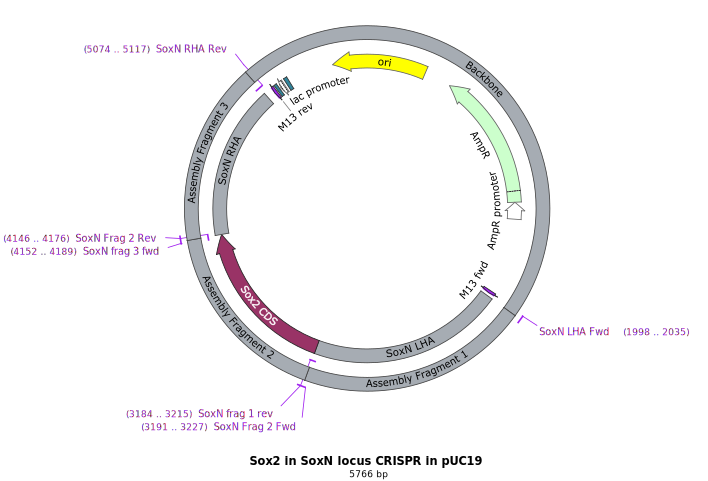
\includegraphics[width=0.8\textwidth]{Fig4_Sox2 in SoxN locus CRISPR in pUC19 Map}
\label{fig4}
\caption{\textbf{Schematic of ``Sox2 in SoxN'' plasmid construct.} Assembly fragments and primers indicate the intended synthesis plan for NEBuilder Gibson-like assembly. mSox2 CDS is positioned for homology-driven repair with the LHA and RHA of the enodgenous SoxN sequence.}
\end{figure}


The general approach to creating such templates relied on synthesising
individual fragments and then annealing them together in order to create
the final plasmid. For both ``Sox2 in SoxN'' and ``Sox2 in D''
constructs, the target plasmid consisted of four major components: the
\emph{SoxN/D} LHA, the \emph{mSox2} CDS, the \emph{SoxN/D} RHA, and a
pUC19 backbone with a multiple cloning site that can be cleaved by the
enzyme \emph{Sma}I. Aside from the backbone, each of these fragments was
synthesised with a minimum 25 nt overlap with the adjacent fragment,
allowing for a final ligation of these overlapping ends using a
Gibson-like assembly protocol provided by New England Biolabs (R. Chao
et al., 2015). Once assembled, the resultant plasmids could be verified
with PCR, used to transform \emph{Escherichia coli} cells, and amplified
to create a high-concentration stock of the assembled plasmid. The bulk
of these wet lab experiments focus on the process of synthesising
fragments and ligating them to create donor templates. Figures 4 and 5
depict schematics of the desired target plasmids, along with the PCR
primers used to generate each of the fragments. Supplementary Figure 1
shows the features of plasmid 1444, the template DNA that was used to
clone the \emph{mSox2} sequence.

\setcounter{figure}{5-1}
\begin{figure}[htbp]
\centering
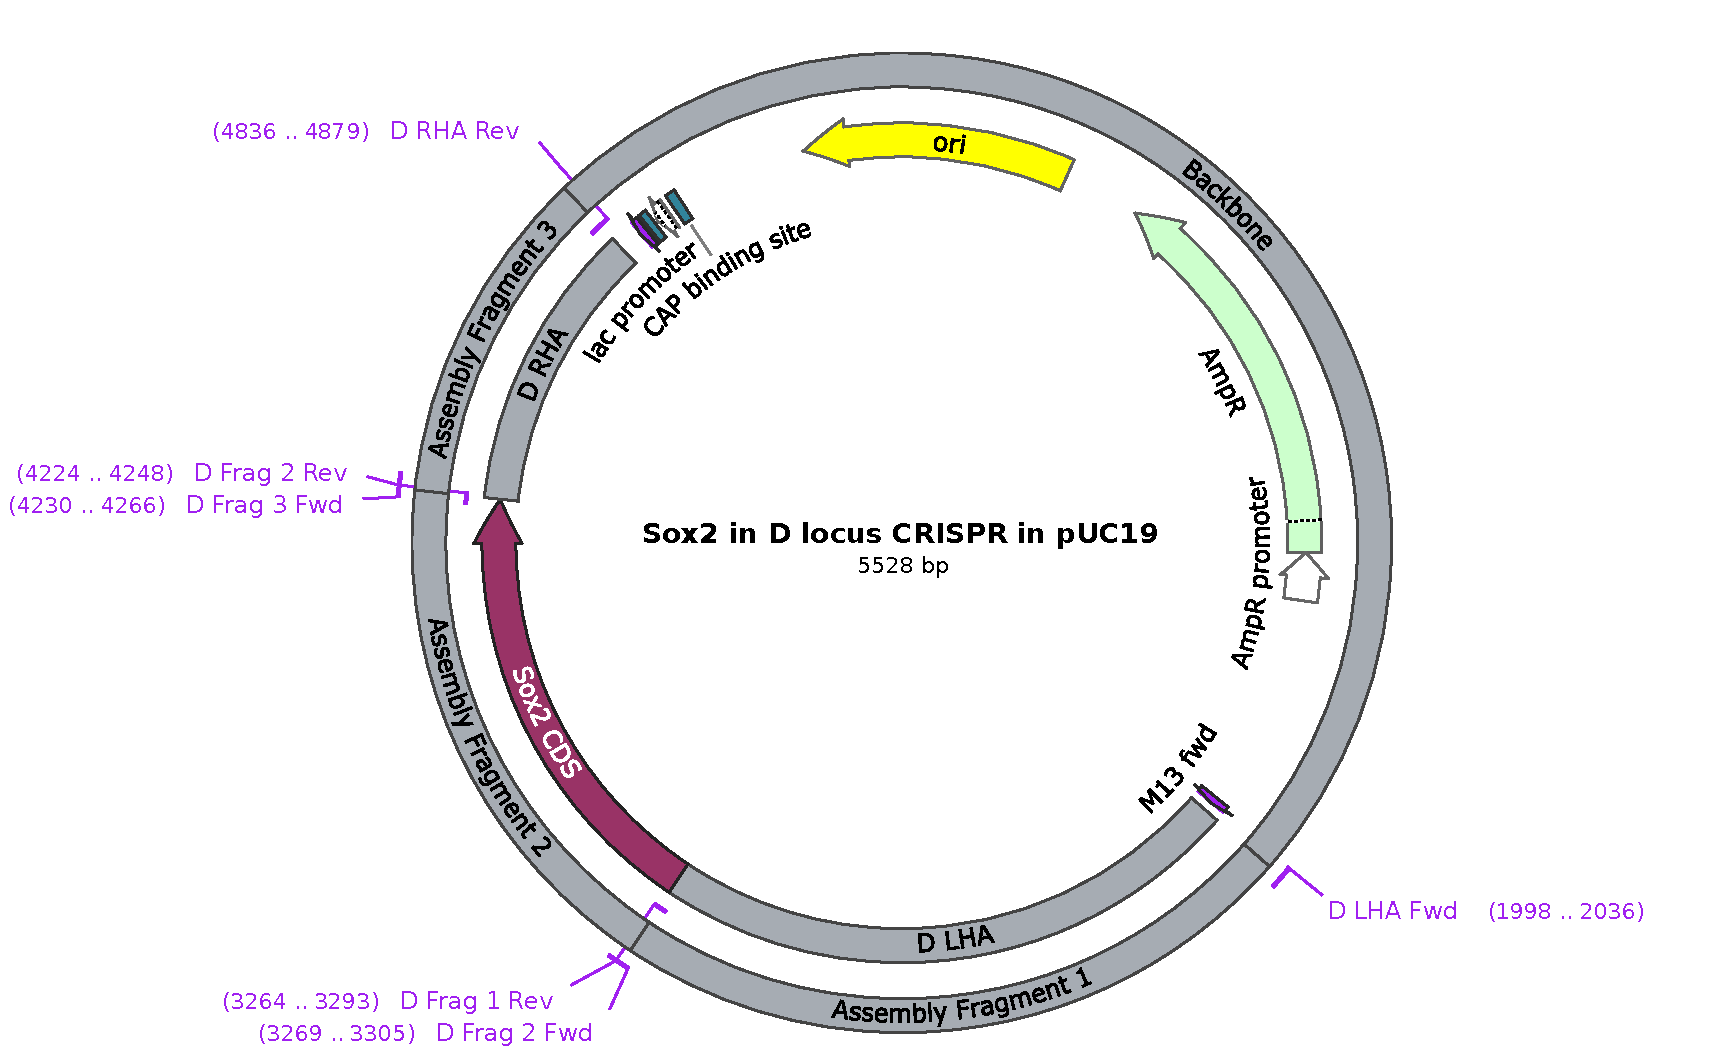
\includegraphics[width=0.8\textwidth]{Fig5_Sox2 in D locus CRISPR in pUC19 Map.pdf}
\label{fig5}
\caption{\textbf{Schematic of ``Sox2 in D'' plasmid construct.} As with the SoxN construct, this places the mSox2 CDS between the LHA and RHA for the endogenous D locus.}
\end{figure}

\section{Materials and Methods}

Reagents and PCR parameters for these experiments are summarised in
Tables 1-5. All materials were from existing stocks or new orders in the
Russell lab. Plasmid 1444, a source of the \emph{mSox2} CDS , was
provided by the lab of Prof. Jennifer Nichols (Cambridge Stem Cell
Inst).

\begin{table}[htbp]
\rowcolors{2}{trowdark}{trowlight}
\centering
\begin{adjustbox}{width=\textwidth, center=\textwidth}
\begin{tabular}{@{}lll@{}}
\rowcolor{thead}
{\color{headtext} \textbf{Reagent}}                         & {\color{headtext} \textbf{Supplier}}    & {\color{headtext} \textbf{Purpose}}         \\
pUC19 + SmaI digest                      & Russell Lab          & Assembly vector          \\
NEB 5-alpha chemically competent E. coli & New England Biolabs  & Bacterial transformation \\
D in SoxN plasmid                        & Russell Lab          & DNA source for PCR       \\
Plasmid 1444                             & Jennifer Nichols Lab & DNA source for PCR       \\
SoxN in D plasmid                        & Russell Lab          & DNA source for PCR       \\
NEBuilder Assembly Cloning kit           & New England Biolabs  & Fragment Assembly        \\
6x loading dye                           & New England Biolabs  & Gel electrophoresis      \\
Agarose                                  & Sigma-Aldrich        & Gel electrophoresis      \\
Ethidium Bromide (EtBr)                  & Sigma-Aldrich        & Gel electrophoresis      \\
GeneRuler 1kb, 100bp ladders             & ThermoFisher         & Gel electrophoresis      \\
Lysogeny broth (\gls{LB}) media and LB agar    & Sigma-Aldrich        & Growing E. coli          \\
Q5 Hi-Fidelity DNA Polymerase Kit        & New England Biolabs  & PCR                      \\
Ampicillin                               & Sigma-Aldrich        & Resistance selection     \\
CloneJet PCR cloning kit                 & ThermoFisher         & Sequencing               \\
Nuclease-free water                      & Sigma-Aldrich        & Solution preparation     \\ \bottomrule
\end{tabular}
\end{adjustbox}
\caption{\textbf{Reagents and suppliers used in experiments}}
\end{table}

\begin{table}[htbp]
\rowcolors{2}{trowdark}{trowlight}
\centering
\begin{adjustbox}{width=\textwidth, center=\textwidth}
\begin{tabular}{ll}
\rowcolor{thead}
{\color{headtext} \textbf{Item}}                              & {\color{headtext} \textbf{Composition}}                                                                                                                                                                                                                                                                                                              \\
1x Tris-Acetate-EDTA (\gls{TAE}) buffer solution & \begin{tabular}[c]{@{}l@{}}- 2 M Tris base\\ - 1 M EDTA\\ - 1 M Acetic acid\\ - MilliQ water to 1 L total\end{tabular}                                                                                                                                                                                                            \\
LB agar                                    & \begin{tabular}[c]{@{}l@{}}- 10 g LB agar powder\\ - 250 mL MilliQ water\\ - 250 $\upmu{}$L of 100 mg/mL ampicillin\end{tabular}                                                                                                                                                                                                          \\
LB Media                                   & \begin{tabular}[c]{@{}l@{}}- 4 $\upmu{}$L aliquot LB liquid media\\ - 4 $\upmu{}$L of 100 mg/mL ampicillin\end{tabular}                                                                                                                                                                                                                           \\
Agarose gel                                & \begin{tabular}[c]{@{}l@{}}- 0.48 g agarose\\ - 60 mL 1x TAE\\ - 2.5 $\upmu{}$L Ethidium Bromide\end{tabular}                                                                                                                                                                                                                             \\
Q5 mix                                     & \begin{tabular}[c]{@{}l@{}}- 1X Q5 Reaction buffer	\\ - 1X Q5 High GC Enhancer\\ - 200 $\upmu{}$M dNTP mix\\ - 0.5 $\upmu{}$M forward primer\\ - 0.5 $\upmu{}$M reverse primer\\ - 0.02 units/$\upmu{}$L Q5 Polymerase\\ - 90 ng template DNA; equivalent\\ volume of nuclease-free water\\ for negative controls\\ - Nuclease-free water to 25 $\upmu{}$L total\end{tabular} \\
Alkaline Lysis Solution I + 2\% RNAse      & \begin{tabular}[c]{@{}l@{}}- 25 mMTris-Hcl\\ - 10 mM EDTA\end{tabular}                                                                                                                                                                                                                                                         \\
Alkaline Lysis Solution II                 & \begin{tabular}[c]{@{}l@{}}- 0.2 N NaOH\\ - 1\% w/v SDS\end{tabular}                                                                                                                                                                                                                                                           \\
Alkaline Lysis Solution III                & - 3 M KOAc, pH 5.2                \\ \bottomrule                                                                                           
\end{tabular}
\end{adjustbox}
\caption{\textbf{Composition of solutions and mixtures used during experimentation}}
\end{table}

\begin{table}[htbp]
\centering
\begin{adjustbox}{width=\textwidth, center=\textwidth}
\rowcolors{2}{trowdark}{trowlight}
\begin{tabular}{lll}
\rowcolor{thead}
{\color{headtext} \textbf{Primer Name}} & {\color{headtext} \textbf{Primer Sequence}}                                                                & {\color{headtext} \textbf{Intended Fragment}} \\
SoxN LHA Fwd         & \begin{tabular}[c]{@{}l@{}}tgaattcgagctcggtaccc\\ GGATCGATATAGTGACGG\end{tabular}    & SoxN LHA \\
SoxN Frag 1 Rev      & \begin{tabular}[c]{@{}l@{}}catgttatacatCTTGCGGG\\ GATTACTTCCAG\end{tabular}          & SoxN LHA                   \\
SoxN Frag 2 Fwd      & \begin{tabular}[c]{@{}l@{}}taatccccgcaagATGTATA\\ ACATGATGGAGACGGAG\end{tabular}     & SoxN\textsuperscript{mSox2} CDS              \\
SoxN Frag 2 Rev      & \begin{tabular}[c]{@{}l@{}}tattttcaataatTCACATG\\ TGCGACAGGGG\end{tabular}              & SoxN\textsuperscript{mSox2} CDS              \\
SoxN Frag 3 Fwd      & \begin{tabular}[c]{@{}l@{}}tcgcacatgtgaATTATTGA\\ AAATATTAACTAAAGCCC\end{tabular}       & SoxN RHA                   \\
SoxN RHA Rev         & \begin{tabular}[c]{@{}l@{}}gtcgactctagaggatcccc\\ GAGATGTTTTTGTAAAGATTTTTC\end{tabular} & SoxN RHA                   \\
D LHA Fwd            & \begin{tabular}[c]{@{}l@{}}tgaattcgagctcggtaccc\\ CGATTGCCCTTGTCCTTTC\end{tabular}      & D LHA                      \\
D Frag 1 Rev         & \begin{tabular}[c]{@{}l@{}}catgttatacatTCCAGCTA\\ TTTTGAACAC\end{tabular}               & D LHA                      \\
D Frag 2 Fwd         & \begin{tabular}[c]{@{}l@{}}caaaatagctggaATGTATA\\ ACATGATGGAGACGGAG\end{tabular}        & D\textsuperscript{mSox2} CDS                 \\
D Frag 2 Rev         & \begin{tabular}[c]{@{}l@{}}ctaaaactcgactTCACATG\\ TGCGACAGGGG\end{tabular}              & D\textsuperscript{mSox2} CDS                 \\
D Frag 3 Fwd         & \begin{tabular}[c]{@{}l@{}}tcgcacatgtgaAGTCGAGT\\ TTTAGGTTAGAGTACAG\end{tabular}        & D RHA                      \\
D RHA Rev            & \begin{tabular}[c]{@{}l@{}}gtcgactctagaggatcccc\\ ATCTTCCAAGCTGTAAATTATTTG\end{tabular} & D RHA \\ \bottomrule{}
\end{tabular}
\end{adjustbox}
\caption{\textbf{PCR primers used for fragment cloning.} Uppercase nucleotides represent where the primers anneal to the source DNA for their intended fragment, while lowercase nucleotides represent overlap with other fragments during ligation.}
\end{table}

\begin{table}[htbp]
\rowcolors{2}{trowdark}{trowlight}
\centering
\begin{adjustbox}{width=\textwidth, center=\textwidth}
\begin{tabular}{lllll}
\rowcolor{thead}
{\color{headtext} \textbf{\begin{tabular}[c]{@{}l@{}}Fragment \\ Name\end{tabular}}} & {\color{headtext} \textbf{DNA Source}} & {\color{headtext} \textbf{Fwd Primer}} & {\color{headtext} \textbf{Rev Primer}} &{\color{headtext}  \textbf{\begin{tabular}[c]{@{}l@{}}Expected \\ length (bp)\end{tabular}}}\\
SoxN LHA               & D in SoxN           & SoxN LHA Fwd        & SoxN Frag 1 Rev     & 1186                          \\
SoxN\textsuperscript{mSox2}              & Plasmid 1444        & SoxN Frag 2 Fwd     & SoxN Frag 2 Rev     & 960                           \\
SoxN RHA               & D in SoxN           & SoxN Frag 3 Fwd     & SoxN RHA rev        & 934                           \\
D LHA                  & SoxN in D           & D LHA Fwd           & D Frag 1 Rev        & 1264                          \\
D\textsuperscript{mSox2}                 & Plasmid 1444        & D Frag 2 Fwd        & D Frag 2 Rev        & 960                           \\
D RHA                  & SoxN in D           & D Frag 3 Fwd        & D RHA Rev           & 618 \\ \bottomrule{}          
\end{tabular}
\end{adjustbox}
\caption{\textbf{Components for synthesising each amplification fragment.}}
\end{table}

\begin{table}[htbp]
\rowcolors{2}{trowdark}{trowlight}
\centering
\begin{adjustbox}{width=\textwidth, center=\textwidth}
\begin{tabular}{llll}
\rowcolor{thead}
{\color{headtext} \textbf{Fragment}} & {\color{headtext} \textbf{Anneal temperature (\textdegree{}C)}} & {\color{headtext} \textbf{Anneal time (s)}} & {\color{headtext} \textbf{Extension time (s)}} \\
SoxN LHA          & 65                                                                         & 30                                                                 & 90                                                                    \\
SoxN\textsuperscript{mSox2}         & 65                                                                         & 30                                                                 & 90                                                                    \\
SoxN RHA          & 58                                                                         & 30                                                                 & 90                                                                    \\
D LHA             & 65                                                                         & 30                                                                 & 90                                                                    \\
D\textsuperscript{mSox2}            & 65                                                                         & 30                                                                 & 90                                                                    \\
D RHA             & 58.2                                                                       & 40                                                                 & 7      \\ \bottomrule{}                                                              
\end{tabular}
\end{adjustbox}
\caption{\textbf{Summary of PCR parameters for different fragments.} All PCR setups start with a single 30-second denaturation step at 98 \textdegree{}C, followed by 32 three-step cycles of melting for 10 seconds at 98 \textdegree{}C, annealing at variable temperatures/times, and extending at 72 \textdegree{}C at variable times. All cycles finish with a final 120 second extension at 72 \textdegree{}C.}
\end{table}

\subsection{Polymerase Chain Reaction}

All \gls{PCR} reactions were performed using the Q5 High-Fidelity Polymerase
protocol from New England Biolabs as summarised in Table 2. Bulk mixes
of Q5 mix were prepared in 500 $\upmu{}$L aliquots containing all reagents
except for primers and template DNA. Template DNA and primer
combinations as summarised in Table 4 were used to create the 25 $\upmu{}$L
reaction mix for each fragment in separate PCR tubes. Initial conditions
were based on the NEB T\textsubscript{m} calculator tool. However,
differences in length and GC content between fragments necessitated
gradient PCR assays at different elongation times to optimise reaction
conditions, with optimal settings for each fragment summarised in Table
5. Each PCR included a negative no-template control. Following PCR, 1 $\upmu{}$L
of each reaction was visualised using gel electrophoresis, while the
remainder was stored at \textminus{}20 \textdegree{}C for future ligation.

Following bacterial transformation, PCR was used to identify positive
colonies with SoxN/D Frag 2 primers used to identify the \emph{mSox2}
CDS. Colonies were mixed in 10 $\upmu{}$L of nuclease-free water, streaked on a
separate LB agar plate for preservation, and heated for 10 minutes at 95
\textdegree{}C to rupture cell walls; 1 $\upmu{}$L of this solution was then used in the
place of the usual template DNA. Colonies that passed the \emph{mSox2}
CDS screen were then PCR tested for the LHA-Sox2 and Sox2-RHA junctions.
Because colony PCR resulted in many false positives, an alternative
method was to first grow each colony in liquid media, miniprep a
purified plasmid, and then perform PCR screens for \emph{mSox2} on the
resultant plasmid.

\subsection{Gel electrophoresis and imaging}

Following PCR, the product of each reaction was visualised using agarose
gel electrophoresis in 1x TAE with Ethidium bromide (\gls{EtBr}) included for
visualisation. The NEB GeneRuler ladder was used as a size marker and
gels were visualised under UV light with the Syngene NuGenius imaging
platform.

\subsection{Fragment assembly}

Once all fragments for a given target plasmid were synthesised, they
were ligated using the NEBuilder HiFI DNA Assembly cloning kit. The
three PCR product fragments were combined with SmaI-digested
pUC19 in a 1:1 vector:insert ratio, following the guidelines for a
four-fragment assembly. The total fragment amount was slightly under 0.5
pmol, and the fragments were combined with HiFi DNA Assembly master mix
and nuclease-free water to a total reaction volume of 20 $\upmu{}$L. A parallel
assembly using the kit's pre-made positive control mix was also
performed. The assembly reactions were kept at 50 \textdegree{}C for at least 60
minutes to facilitate ligation. Following the ligation process, 1 $\upmu{}$L of
the reaction product was used for bacterial transformation, and the
remainder was stored at \textminus{}20 \textdegree{}C.

\subsection{Bacterial transformation}

NEB DH5-alpha \emph{E. coli} cells were transformed with the ligated
plasmids. Thawed chemically competent cells from the NEBuilder assembly
kit were mix with 1 $\upmu{}$L of plasmid product, chilled on ice for 30
minutes, heat shocked at 42 \textdegree{}C for 30 seconds to induce transformation,
and then chilled for another 2 minutes on ice. The transformed \emph{E.
coli} cells were added to 300 $\upmu{}$L of SOC outgrowth medium and incubated
for an hour at 37 \textdegree{}C in a 300 RPM shaker. A 100 $\upmu{}$L portion of the
culture was plated and spread on a warmed LB agar and ampicillin
plate, and then incubated overnight for no longer than 20 hours. For the
NEBuilder assembly products, the process was repeated in parallel with
the positive control product. Positive colonies were grown in liquid
media and combined in a 1:1 ratio with 50\% glycerol for long-term
storage at \textminus{}80 \textdegree{}C.

\subsection{Miniprep plasmid extraction}

After overnight growth of \emph{E. coli} in liquid media, alkaline lysis
was used to isolate and extract plasmid DNA. A total of 3 mL of \emph{E.
coli} culture was pelleted at 8000 RPM and then resuspended in 150 $\upmu{}$L of
Solution I + 2\% RNAse. This was gently mixed with 150 $\upmu{}$L of Solution II
to lyse cell walls followed by 150 $\upmu{}$L of Solution III to neutralise the
pH of the mixture. The reaction was chilled at \textminus{}20 \textdegree{}C for 5 minutes, and
the DNA was precipitated with 500 $\upmu{}$L of isopropanol, followed by another
\textminus{}20 \textdegree{}C chill for 10 minutes and a 5 minute centrifugation at 13000 RPM.
The supernatant was discarded and the remaining pellet was washed with
400 $\upmu{}$L of 100\% ethanol to remove excess salt. This was followed by
centrifuging again for 5 minutes at 13000 RPM and discarding the
supernatant. The pellet was completely dried for 10 minutes in an open
tube and then resuspended in 20 $\upmu{}$L of nuclease-free water to produce the
final product.

\subsection{Sanger sequencing}

Two different approaches were used for sequencing, one involving cloning
the \emph{mSox2} CDS into a ThermoFisher CloneJET system for sequencing
with pJET1.2 universal primers, and one involving new primers
specifically for sequencing from the plasmid 1444 template. In both
cases, each Sanger sequencing attempt took two separate 10 $\upmu{}$L reactions:
6.5 $\upmu{}$L of nuclease-free water, 1 $\upmu{}$L of template DNA at a starting
concentration of 90 ng/$\upmu{}$L, and 2.5 $\upmu{}$L of either the forward or reverse
10 $\upmu{}$M primer.

To clone the \emph{mSox2} DNA into the pJET1.2 vector, 1 $\upmu{}$L of raw PCR
product from the reaction that used SoxN\textsuperscript{mSox2} primers
was combined on ice with 10 $\upmu{}$L of reaction buffer, 1 $\upmu{}$L of T4 DNA
ligase, 1 $\upmu{}$L of the pJET1.2 blunt cloning vector, and 7 $\upmu{}$L of
nuclease-free water. The ligation reaction occurred for 5 minutes at
room temperature, and was then used to transform chemically competent
DH5-alpha \emph{E. coli} cells. After incubation at 37 \textdegree{}C overnight on
an ampicillin selection plate, a colony was selected, grown in liquid
media, and plasmid DNA was extracted via miniprep. This was used for
sequencing in conjunction with the pJET1.2 forward primer
5'-d(CGACTCACTATAGGGAGAGCGGC)-3' and the reverse primer
5'-d(AAGAACATCGATTTTCCATGGCAG)-3'. The sample was sent to the Genewiz
sequencing service for analysis.

When this approach failed to yield any results, it was repeated with new
custom primers designed specifically for the plasmid 1444 template. The
computational tool Primer3 was used to optimise a set of primers between
100-300 bp outside of the \emph{mSox2} CDS \shortcite{untergasser_primer3new_2012}.
The sequences for these primers are 5'-d(GCTTCTGGCGTGTGACCG)-3' for the
primer ``Sox2 Sanger Fwd'' and 5'-d(CACACCGGCCTTATTCCAAG)-3' for ``Sox2
Sanger Rev.'' While this approach did result in a sequence output, the
sequence was half as long as expected and low-fidelity. No further
sequencing attempts occurred due to the onset of COVID-19 shutdowns the
following week.

\section{Results}

Fragments were synthesised from DNA templates, and PCR conditions were
optimised so that consistent fragments could be generated from a base
plasmid or from colony miniprep templates. The expected length of each
fragment is shown in Table 4, and the optimised PCR conditions are
summarised in Table 5. For both the ``Sox2 in SoxN'' and ``Sox2 in D''
donor template plasmids, synthesis of each individual fragment was
successful, but transformation of the ligation product proved more
problematic. The SoxN plasmid successfully ligated, generated
transformed bacterial colonies, and was analysed for the presence of
each component fragment (Figure 6). Unfortunately, contamination in the
bacterial stocks meant that this assembled plasmid was lost. It is not
certain that the presence of the LHA, \emph{mSox2} CDS\emph{,} and RHA
fragments were sufficient to determine that the assembly was successful,
as secondary primer pairs to test the junction between the CDS and each
homology arms yielded fragment sizes that were inconsistent; however, it
is unclear that this is due to unsuccessful assembly, as significant
contamination was observed in these experiments, which were conducted
right before the COVID shutdown. Conversely, each of the D fragments
were successfully synthesised (Figure 7), but efforts to introduce the
ligated products into bacteria and select positive colonies proved
unsuccessful. PCR products of each fragment necessary to construct
either construct are still available, and can be used to create fresh
plasmids. Because the final PCR conditions are now known, the fragments
can readily be freshly synthesised and ligated without further
optimisation.

\setcounter{figure}{6-1}
\begin{figure}[htbp]
\centering
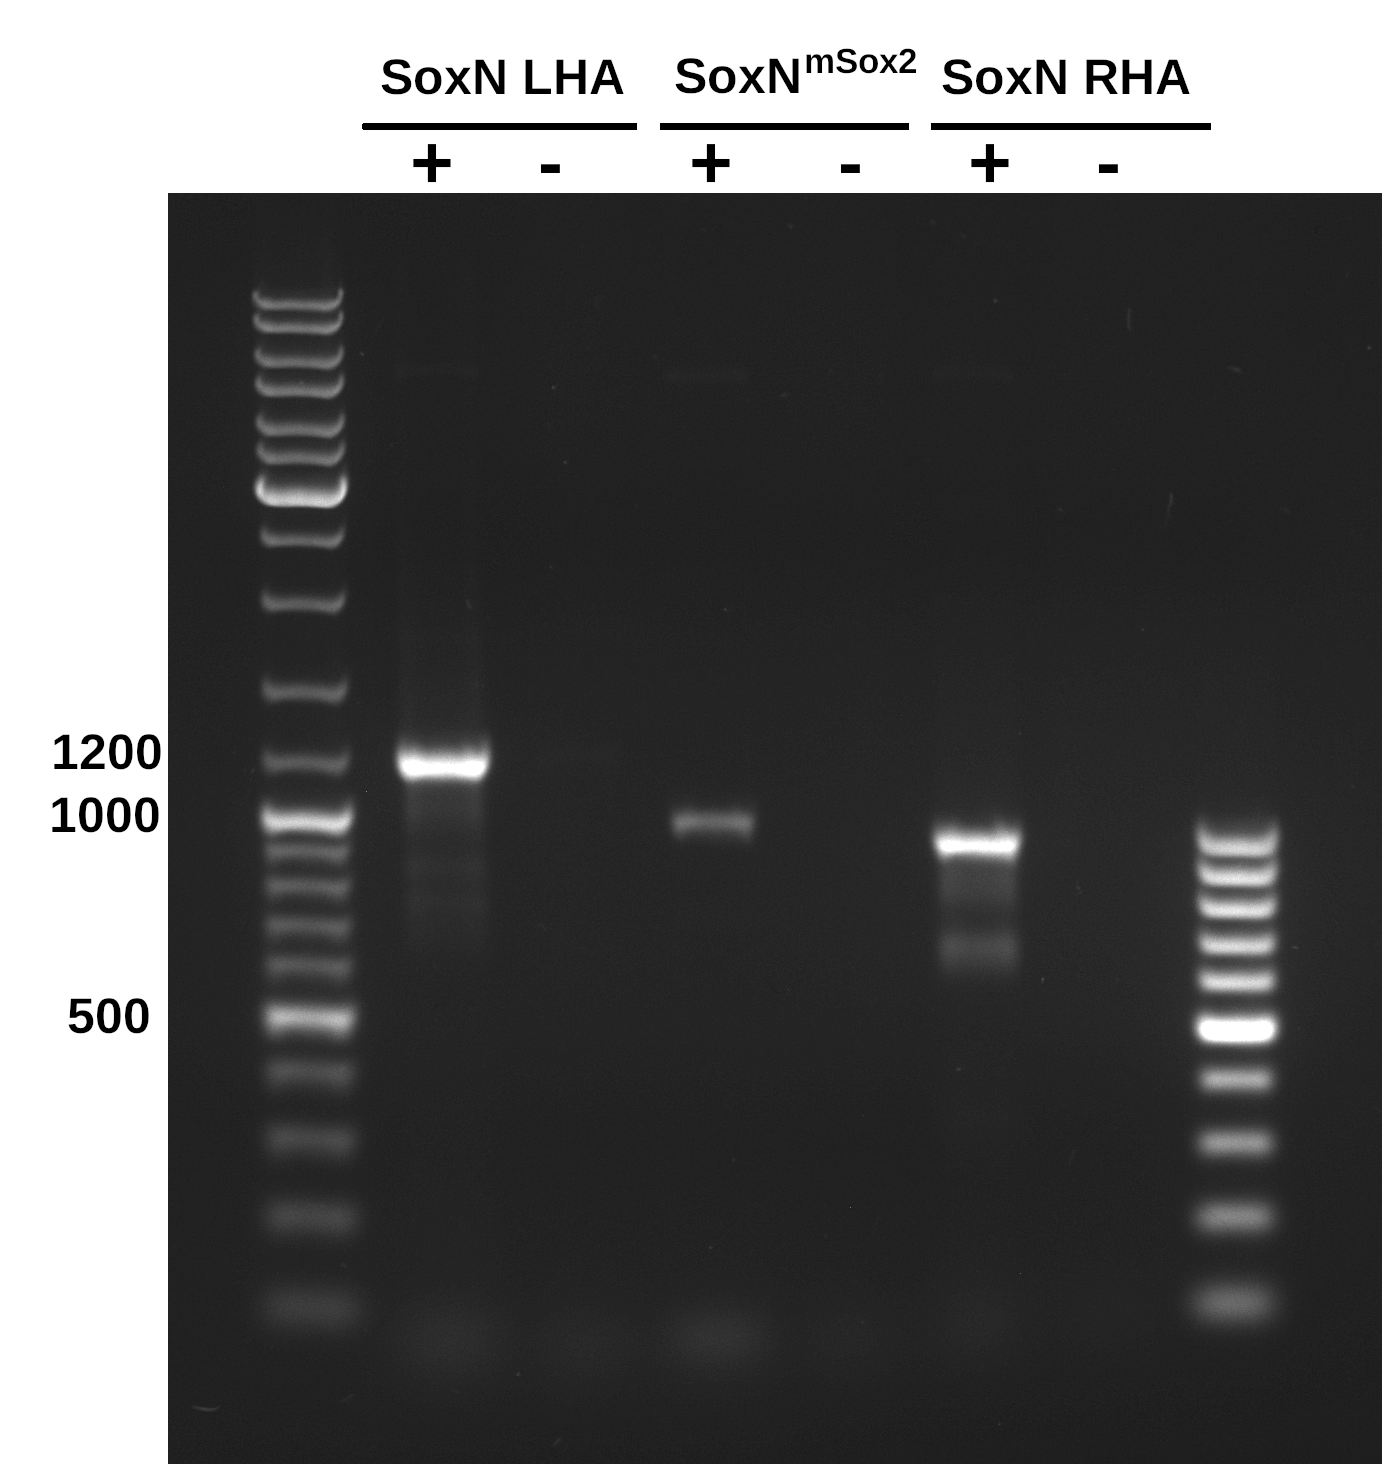
\includegraphics[width=0.5\textwidth]{Fig6_Jan30-SoxN_Assembly.png}
\label{fig6}
\caption{\textbf{PCR verification of each fragment in assembled ``Sox2 in SoxN'' plasmid.} Lane order: GeneRuler 1kb, SoxN LHA, SoxN LHA n.c., SoxN\textsuperscript{mSox2}, SoxN\textsuperscript{mSox2} n.c., SoxN RHA, SoxN RHA n.c., GeneRuler 100bp.}
\end{figure}

\setcounter{figure}{7-1}
\begin{figure}[htbp]
\centering
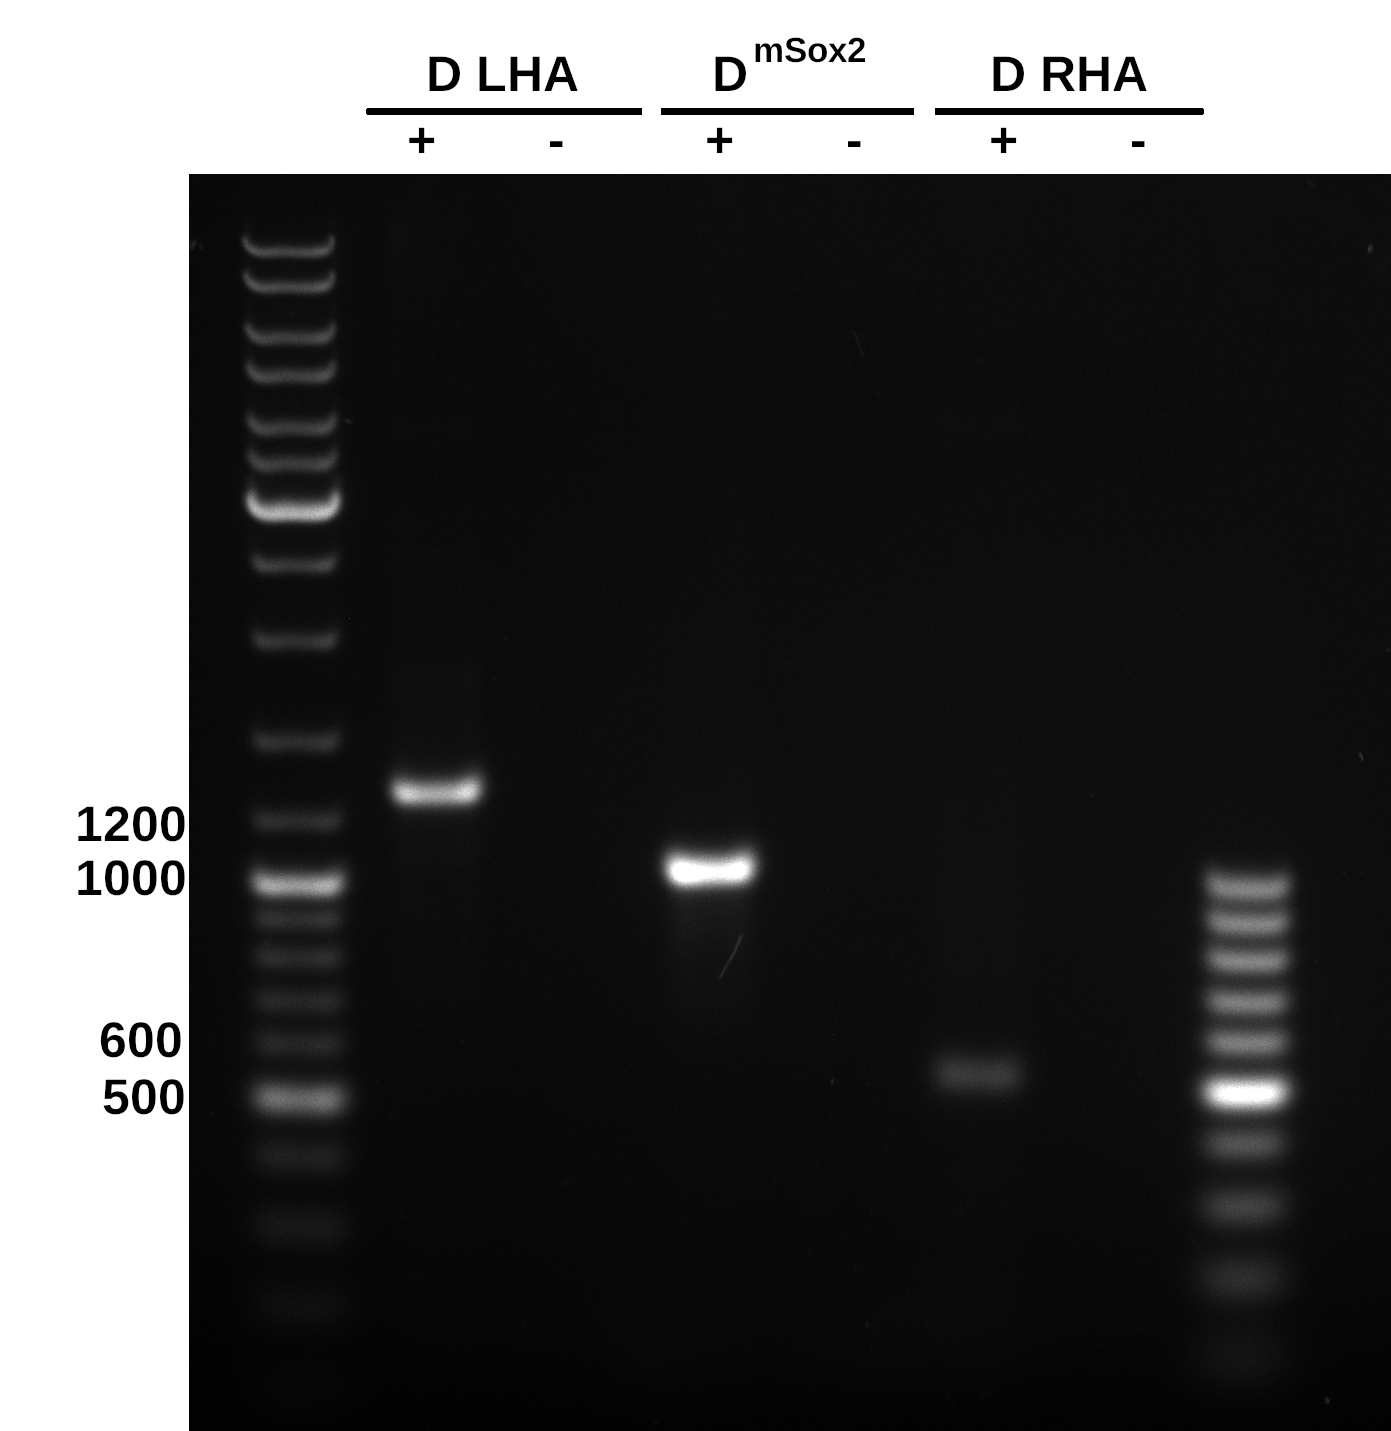
\includegraphics[width=0.5\textwidth]{Fig7_Mar04-D unassembled frags.png}
\label{fig7}
\caption{\textbf{Unassembled fragments for ``Sox2 in D'' construct.} These represent the stable PCR products for each  assembly fragment prior to ligation. Assembly into final plasmid was unsuccessful, but fragments prior to ligation were of expected lengths. Lane order: GeneRuler 1kb, D LHA, D LHA n.c., D\textsuperscript{mSox2}, D\textsuperscript{mSox2} n.c., D RHA, D RHA n.c., GeneRuler 100bp.}
\end{figure}


While all fragments were eventually optimised, certain fragments took
more effort to ensure ideal conditions. Various two-step and three-step
synthesis protocols were attempted, with different annealing
temperatures and extension times. LHA fragments and \emph{mSox2} CDS
fragments for both the SoxN and D constructs were readily synthesised at
a 65 \textdegree{}C anneal temperature and 90 second extension time. The RHA
fragments were considerably more difficult to produce. The SoxN RHA
fragment was not generated with a 65 \textdegree{}C anneal temperature, but was
found when the annealing condition was changed to 58 \textdegree{}C. The D RHA
fragment required multiple combinations of both annealing temperature
and extension time before stable conditions were found. Gradient PCR
revealed that 58.2 \textdegree{}C annealing temperature combined with an extension
time of 19 seconds initially generated a PCR product (Figure S2),
however, this was not reproducible and the gradient PCR scheme was
modified under different extension times to yield a more reliable
product with an extension time of only 7 seconds.

Colony PCR was used to select \emph{E. coli} colonies that contained
either the assembled SoxN or D constructs. Primers for the \emph{mSox2}
CDS fragment were used as a first-past screen, after which positive
colonies were grown and miniprepped to yield a more pure DNA template
for a second-pass screen that also included the LHA and RHA fragments.
However, the colony PCR method yielded a high rate of false positives.
While several colonies would appear to be positive for the \emph{mSox2}
CDS fragment (Figure S3), this fragment was not present in a stable form
once the same PCR was repeated on purified miniprep DNA (Figure S4).
Therefore, it became more reliable during the selection process to first
grow out each colony in liquid media, use a miniprep extraction to
obtain purified plasmid DNA, and then perform the first-pass
\emph{mSox2} screen using the purified DNA. While this technique yielded
fewer false positives, a significant drawback was that it was more
time-intensive. Differences in transformation efficiency were observed
depending on the \emph{E. coli} cells being used, as transformation with
cells that were made chemically competent in the lab yielded no colonies
on an ampicillin selection plate, while the high-efficiency DH5-alpha
competent cells from the NEBuilder kit were consistently able to produce
colonies on selection plating.

Attempts to sequence the \emph{mSox2} CDS from plasmid 1444 proved
ultimately unsuccessful. As described previously, Genewiz Sanger
sequencing attempts failed due to lack of primer annealing for the
pJET1.2 universal primer construct. Secondary sequencing attempts with
the custom primers optimised specifically for plasmid 1444 were able to
bind, but produced an essentially meaningless output, with 282 of the
435 bases marked as N despite the fact that the primers were over 1300
bp apart from each other (Figures S1, S5). It is unclear why these
primers failed to result in a high-quality Sanger sequence, but
verification of the identity and integrity of the \emph{mSox2} CDS
sequence from plasmid 1444 will be necessary before the ligated donor
templates are ultimately used to create CRISPR knock-ins.

\section{Discussion}

Difficulties during PCR synthesis arose due to a combination of the
properties of the PCR primers and of the intended target fragments.
Because the assembly primers created by the NEBuilder assembly tool
contained a minimum overlap of 25 nt, each primer had a relatively large
estimated estimate from the NEB T\textsubscript{m} calculator, and
therefore the first attempt for most fragments involved a two-step
synthesis that combined annealing and extension at 72 \textdegree{}C. Through trial
and error, it became evident that these T\textsubscript{m} values were
actually lower in practice as compared to the calculated theoretical
values.

In addition to difficulties due to the T\textsubscript{m}, the next
biggest difficulty with PCR was due to the sequence of the fragments
themselves. For both the SoxN and D RHA fragments, the lower annealing
temperature of near 58 \textdegree{}C was likely related to the low GC content of
the target fragment, as the SoxN RHA fragment was 34\% GC and the D RHA
was 33\% GC while other fragments were closer to 50\%. This finding is
consistent with previous observations that high GC content of the
desired PCR product correlates with higher annealing temperature
(Mammedov et al., 2008). Gradient PCR (Figure S2) was instrumental in
rapidly varying the annealing temperature condition to identify viable
conditions; if a band of the proper size was present but faint, slightly
altering the reaction conditions could produce a more consistent
product.

While PCR yielded reliable results when the DNA template was a purified
plasmid, false positives were frequent when attempting colony PCR
screens. When performing a screen for \emph{mSox2} CDS in transformed
colonies, it was common to see positive colonies (Figure S3), but when
the PCR was repeated for the purified plasmids for each colony, there
was a high degree of nonspecific bands, as well as a low intensity for
bands of the desired size (Figure S4), indicating that many of the
supposedly Sox2-positive colonies did not actually incorporate the CDS
successfully. One likely explanation for the high degree of false
positives is that unassembled fragments from the ligation step may have
been present in the outgrowth media that was used to plate the
transformed cells. This is consistent with the fact that many of these
positives disappeared after purifying the internal plasmid DNA.

Because of difficulties with Sanger sequencing, it was not possible to
verify conclusively that the \emph{mSox2} CDS contained the true
\emph{Sox2} sequence, but the proper PCR fragment length was produced
consistently whether using the SoxN or D assembly primers, indicating
some degree of consistency in the product under equivalent sets of
primers. Possible explanations for the lack of Sanger sequence using
pJET universal primers, and for the low-quality results when the process
was repeated with custom primers for plasmid 1444 (Figure S5), involve
the idea that Sanger sequencing simply has a lower tolerance for primer
defects as compared to PCR. With PCR, reaction conditions can be
modified in terms of buffer components and cycle parameters, but Sanger
sequencing is a purely linear process that proceeds uniformly. Defects
in primer binding will result in a lower quality product under Sanger
sequencing as compared to PCR, which can better tolerate sub-optimal
binding and reaction conditions. A priority for future assembly attempts
will be verifying that the sequence is indeed identical to the known
\emph{mSox2} nucleotide sequence. If problems persist, it may be
necessary to obtain another \emph{mSox2} CDS from a source plasmid that
is more amenable to sequencing.

\subsection{Future Work}

Assuming that it is possible to verify the \emph{mSox2} sequence and to
eventually create the desired donor plasmids, the next step would
involve providing both plasmids and their associated gRNAs to the
Genetics Department microinjection service for insertion into embryos
expressing Cas9. Crossing these to relevant balancer stocks
(\emph{Sco/SM6a} for \emph{SoxN} and \emph{TM2/TM6c} for \emph{D}), F1
progeny would be screened for the presence of the \emph{mSox2} sequence
via PCR. There are two possible outcomes for each of the replacements.
One is that they will be homozygous viable and fertile, indicating that
Sox2 is able to provide all wild type \emph{Drosophila} SoxB functions.
Alternatively, there may be observable phenotypes, most likely
lethality, that indicate that Sox2 cannot fully fulfill the role of the
endogenous genes.

Whether the knock-in mutations are viable or lethal, it would first be
necessary to perform a phenotypic assessment of homozygous knock-in
embryos. Immunostaining with the BP102 antibody will allow for an
initial assessment of any CNS phenotypes, since these are well described
for \emph{Dichaete} and \emph{SoxN} null mutants. Further investigation
avenues, such as examining neuroblast markers including \emph{Eagle} and \emph{Worinu}
in both knock-ins \shortcite{buescher_formation_2002,overton_evidence_2002},
expression of segmentation genes like \emph{eve} in the
\emph{Dichaete\textsuperscript{Sox2}} lines \shortcite{russell_dichaete_1996}, or
neuronal markers including \emph{Nerfin-1} or \emph{Sema-1a} for late \emph{SoxN}
functions \shortcite{ferrero_soxneuro_2014}, will help identify processes where
Sox2 cannot adequately provide normal SoxB function. Because the
aforementioned genes have been previously characterised in the context
of SoxB binding and mutant phenotypes, it may be possible to identify
sequence contexts at mapped enhancers to understand any lack of
functional rescue.

To further explore the relationship between the mammalian and fly SoxB
proteins at the level of the genome, it was my plan to perform ChIP-seq
analysis on the knock-in stocks to determine how the binding profile of
mSox2 compares to the endogenous profiles of SoxN and D as described
previously by the lab \shortcite{aleksic_role_2013,ferrero_soxneuro_2014}. For
example, a cross of \emph{SoxN\textsuperscript{mSox2}/SM6a} x
\emph{SoxN\textsuperscript{GFP}/SoxN\textsuperscript{GFP}} would result
in progeny that are 50\%
\emph{SoxN\textsuperscript{Sox2}/SoxN\textsuperscript{GFP}} and 50\%
\emph{SoxN\textsuperscript{GFP}/SM6a}. For stage 9-10 embryos, it will
not be possible to differentiate the progeny by phenotype in sufficient
quantities for ChIP-seq, so an appropriate experimental setup would be
to perform ChIP with both $\upalpha$-mSox2 and $\upalpha$-GFP antibodies using the same
chromatin preparations. ChIP validated antibodies are available for both
Sox2 and GFP \shortcite{lodato_sox2_2013,porcelli_chromatin_2019}. While the
level of \emph{SoxN\textsuperscript{mSox2}} would only be half that of
the endogenous \emph{SoxN}, only one copy of \emph{SoxN}---the one with
the GFP tag---would be immunopurified. Additionally, because the
antibodies have different binding efficiency, it will not be possible to
perform a true normalisation between their binding profiles, but a
qualitative comparison of binding profiles would allow for comparison
between SoxN and Sox2 binding in the same cells, revealing the extent of
functional equivalence at the level of genome binding. This approach
would be repeated for \emph{D\textsuperscript{mSox2}} and
\emph{D\textsuperscript{GFP}}, with similar caveats.

Similar questions have already been asked in other organisms. To study
whether the genomic sequence or the nuclear environment were more
important in determining transcriptional regulation, Wilson \emph{et
al.} added an aneuploid human chromosome 21 to Tc1 mouse hepatocytes,
finding that TF binding and transcription initiation along this
aneuploid chromosome recapitulated the patterns present in chromosome 21
of human hepatocytes \shortcite{wilson_species-specific_2008}. Qiu \emph{et
al.} similarly explored the levels of human chromosome 21 expression as
compared to the expression of endogenous orthologues in Tc1 mouse
neurons, finding a significant correlation that they attributed to
sequence-level similarity between orthologous human and mouse genes; the
differences in expression were attributed to sequence divergence \shortcite{qiu_evidence_2016}.

This implies a mode of regulation in which differences in cellular
environments and nuclear transcription factors between species matters
less than the primary sequence of the exogenous genes or chromosomes, at
least in similar tissues. From this, we might expect that the sequence
differences between fly SoxB genes and \emph{mSox2} may make it unlikely
for \emph{mSox2} to fully rescue the endogenous phenotype, especially
since there is evidence that TF binding divergence between closely
related species is a function of both factor-independent variables like
chromatin state and factor-dependent differences in consensus site
recognition \shortcite{bradley_binding_2010}. Ostensibly, any failure for
\emph{mSox2} to recapitulate endogenous function may relate to the
factor's inability to recognise the proper binding sequence.
Alternatively, regulatory sequence divergence for orthologous genes
appears to impact TF binding affinity without qualitatively changing
which loci are bound \shortcite{bradley_binding_2010,wittkopp_variable_2010}, so under
the regulation of the fly Sox loci, \emph{mSox2} may target and be
targeted by the same network members as \emph{SoxN} and \emph{D}.
Depending on whether or not \emph{mSox2} recapitulates the SoxB
phenotypes, it may be possible either to identify the sequence-level
differences that prevent it from binding dSoxB recognition sequences or
to find the identities of the regulatory targets and cofactors that it
shares with the dSoxB genes.

Taken together, these proposed analyses would help elucidate the extent
to which SoxB genomic binding is determined by the amino acid sequences
of the proteins or by chromatin context. If this successful, it may even
be worthwhile to perform single-cell RNA-sequencing to judge whether
changes in binding targets for the exogenous \emph{mSox2} also correlate
with changes in expression patterns of downstream target genes and
whether there are pleiotropic effects of the knock-in for tissues such
as the eyes or intestine. Such differences may provide a new focus for
other aspects of mutant phenotypic screening. In turn, examining mutant
phenotype differences between the \emph{SoxN\textsuperscript{mSox2}} and
\emph{D\textsuperscript{mSox2}} flies can reveal how the regulatory
pressures on the SoxB loci differ and can also provide a starting point
for further exploration of the tissues and cofactors associated with
each endogenous gene.

\chapter{Computational Experiments}

To provide a perspective complementary to that of the proposed wet lab
experiments, we decided to explore the expression of \emph{SoxN} and
\emph{D} \emph{in vivo}. Previously published single cell RNA-seq
(\gls{scRNA-seq}) datasets \shortcite{allen_single-cell_2020,brunet_avalos_single_2019,karaiskos_drosophila_2017} provide a wealth of information on the
expression of genes in the \emph{Drosophila} nervous system and mining
these datasets may provide insights into the cell types that express
\emph{SoxN} and \emph{D,} suggest biological functions, and identify
other factors that these cells express. Compared to methods such as
immunostaining or the use of lacZ reporters that focus only on a gene of
interest, genomic approaches allows us to define groups of cells that
are positive for a gene of interest and then examine the contribution of
other genes in those same cell groups. By comparing transcriptomic data
across different stages of fly development, it is possible correlate
expression groups with known cell types, and then to examine the other
commonalities of those expression groups.

Transcriptome analysis via scRNA-seq offers a relatively unbiased way to
profile the transcriptional output in a group of cells. Protocols for
scRNA-seq generally involve isolating mRNA via its poly-A tail,
fragmenting transcripts, reverse transcribing the fragments, and
amplifying the cDNA fragments before sequencing \shortcite{hebenstreit_methods_2012}.
Fragmentation helps keep read length short, reducing 5' biases caused by
differences in the polymerase progression \shortcite{mortazavi_mapping_2008} but
comes at the expense of transcript integrity.

In addition to standard scRNA-seq methods, other protocols help optimise
characteristics such as transcript integrity or spatial/temporal
specificity. Switching mechanism at the 5' end of the RNA transcript
(\gls{SMART}) protocols use the Moloney murine leukemia virus (\gls{MMLV}) reverse
transcriptase, which provides an ``anchor'' for polymerase template
switching, allowing for production and amplification of cDNA for the
full length of the transcript, averaging 2 kb at a time \shortcite{zhu_reverse_2001}. SMART-based scRNA-seq protocols like Single-cell tagged reverse
transcription (\gls{STRT}) add a barcode for each sample to allow for parallel
multiplexed sequencing, and contain a one-to-one relation between
sequencing reads and original mRNAs \shortcite{hebenstreit_methods_2012,islam_characterization_2011}. Similar methods like Smart-Seq trade off strand specificity for
increased coverage depth and isoform specificity \shortcite{hebenstreit_methods_2012,ramskold_full-length_2012}. The CEL-seq protocol attempts to avoid the
pitfalls of data loss during exponential PCR amplification by instead
using the linear progression of \emph{in vitro} transcription (\gls{IVT}),
resulting in less variation and greater reproducibility as compared to
STRT \shortcite{hashimshony_cel-seq_2012}. The Drop-Seq protocol separates each
cell into nanoliter droplets and assigns a unique barcode to each cell's
mRNA output, allowing for rapid profiling of the entire transcriptome of
a group of cells \shortcite{macosko_highly_2015}.

The aforementioned protocols all use next-generation sequencing (\gls{NGS}) to
sequence amplified fragments. Other protocols allow for single cell
resolution transcriptomic profiling with a more limited scope.
Fluorescent \emph{in situ} RNA sequencing (\gls{FISSEQ}) relies on \emph{in
situ} reverse transcription to produce cDNA that is then crosslinked and
hybridised to fluorescent probes which are imaged with confocal
microscopy \shortcite{lee_highly_2014}. This offers a high degree of
spatial resolution for transcripts, but fails to profile the entire
transcriptome and involves shorter (\textless{} 30 nt) sequencing reads.
Single molecule fluorescence \emph{in situ} hybridisation (\gls{smFISH})
similarly uses fluorescently tagged DNA oligo probes to find nascent
transcripts, and imaging can provide a detailed view of the spatial
distribution of a given mRNA species as well as real-time information on
its transcriptional rate \shortcite{li_multiplex_2019}. However, these methods
fail to provide the unbiased whole-transcriptome profiling that
NGS-based scRNA-seq methods do.

This analysis looks at three public scRNA-seq datasets to examine SoxB
expression. The embryonic dataset from Karaiskos \emph{et al}. uses the
10X Chromium protocol to examine approximately 8000 cells from stage 6
embryos; the dataset from Avalos \emph{et al.} uses Drop-Seq to sequence
approximately 5000 cells from the first instar larval brain separated
from the ventral nerve cord (\gls{VNC}); and the adult VNC dataset from Allen
\emph{et al}. contains approximately 26000 cells sequenced via 10X
Chromium. Both \emph{SoxN} and \emph{D} are known to be expressed in the
neuroectoderm of stage 6 embryos \shortcite{nambu_drosophila_1996,russell_dichaete_1996,overton_evidence_2002}. While neither gene has been characterised
in first instar larvae, both are highly expressed in the embryonic
brain. \emph{D} is expressed in larval optic lobes \shortcite{melnattur_sox_2013} and late larval brain \shortcite{suzuki_temporal_2013}. \emph{SoxN} is more
widely expressed in the larval brain and VNC \shortcite{cremazy_sox_2000}, and
is present in various neurons of the adult nervous system \shortcite{schilling_transcriptional_2019}. Together, these datasets provide a way to independently
validate existing expression patterns of \emph{SoxN} and \emph{D} while
uncovering nuances in their regulation.

\section{Materials and Methods}

To begin, processed read matrices for each of the three datasets were
downloaded from the NCBI Gene Expression Omnibus. While different data
processing steps were detailed in each of the original papers, for my
analysis I elected to employ the same pipeline for all datasets to
ensure a degree of consistency, unless otherwise noted. The majority of
computational analyses used a local Ubuntu 18.04 installation running
bash version 4.4.20 and R version 3.4.3 on a machine with 8 GB of RAM.
For tasks that required higher computational power, the Rustbucket
server in the University of Cambridge network provided a Debian 9
environment with 32 GB of RAM, running bash version 4.4.12 and R version
4.4.0. A complete list of software packages and versions used in these
analyses is provided in Table 6. For each dataset, processing scripts
and output files are provided at \href{https://github.com/edridgedsouza/mphil-thesis}{\emph{https://github.com/edridgedsouza/mphil-thesis}}.

\begin{table}[htbp]
\rowcolors{2}{trowdark}{trowlight}
\centering
\begin{adjustbox}{width=.75\textwidth, center=\textwidth}
\begin{tabular}{ccc}
\rowcolor{thead}
{\color{headtext} \textbf{Attached Package}} & {\color{headtext} \textbf{Ubuntu Version}} & {\color{headtext} \textbf{Rustbucket Version}} \\
ALL                       & 1.28.0                  & -                           \\
Seurat                    & 3.1.5                   & 3.1.5                       \\
purrr                     & 0.3.4                   & -                           \\
UpSetR                    & 1.4.0                   & -                           \\
ggplot2                   & 3.3.0                   & 3.3.0                       \\
rvest                     & 0.3.5                   & -                           \\
xml2                      & 1.3.0                   & -                           \\
org.Dm.eg.db              & 3.10.0                  & -                           \\
topGO                     & 2.38.1                  & -                           \\
SparseM                   & 1.78                    & -                           \\
GO.db                     & 3.10.0                  & -                           \\
AnnotationDbi             & 1.48.0                  & -                           \\
IRanges                   & 2.20.2                  & -                           \\
S4Vectors                 & 0.24.3                  & -                           \\
Biobase                   & 2.46.0                  & -                           \\
graph                     & 1.64.0                  & -                           \\
BiocGenerics              & 0.32.0                  & -                           \\
tibble                    & 3.0.1                   & 3.0.1                       \\
dplyr                     & 0.8.5                   & 0.8.5                       \\
ClusterMap                & -                       & 0.1.0                      \\ \bottomrule{}
\end{tabular}
\end{adjustbox}
\caption{\textbf{R software packages and corresponding version numbers.} Packages shown are non-base libraries listed under the "other attached packages" output of the \code{sessionInfo()} function. Versions are shown for the local Ubuntu installation running R v3.4.5 and for the Debian installation on the Rustbucket server running R v4.4.0. A complete list of all packages loaded via namespace but not attached to the R session can be found on GitHub}
\end{table}

\subsection{Data Preprocessing}

Data for each analysis was obtained from the NCBI GEO database using
accession numbers GSE95025, GSE134722, and GSE141807 for the embryo,
larval brain, and adult VNC datasets, respectively. The original methods
used for processing for these datasets involved some filtering to
eliminate cells or genes with low expression. However, because this
project seeks to explore the nuances of \emph{SoxN} and \emph{D}
expression, even in cells with low transcript counts, I performed all
analyses using unfiltered data to capture the total variance present in
the original samples.

The embryo study included replicates from both \emph{Drosophila
melanogaster} and \emph{Drosophila virilis,} the larval brain study
included replicates from starved and unstarved individuals, and the
adult VNC study examined both male and female replicates separately. In
order to maintain consistency, the final datasets used for analysis used
pooled expression data across multiple replicates, with no
replicate-specific normalisation. I restricted the embryo analysis to
\emph{D. melanogaster} expression for ease of comparison with other
data, while only unstarved flies were considered for the analysis of the
larval brain dataset. Each replicate of the adult VNC dataset contained
approximately 30,000 sequencing barcodes, an order of magnitude larger
than the other datasets that used approximately 1,000 to 2,000 barcodes
per replicate. While pooling male and female replicates would have been
more biologically comparable to the other datasets, it would also
require much greater computational power. Consequently, only male
replicates from the adult VNC dataset were pooled for analysis. However,
the scripts used to process these data can be easily adapted to consider
only females or both males and females.

The R package Seurat \shortcite{satija_spatial_2015} provides a complete set of
methods for processing and analysing scRNA-seq data, and was the main
package used for this project. Gene identifiers unique to
\emph{Drosophila} were resolved via org.Dm.eg.db from the Bioconductor
repository \shortcite{gentleman_bioconductor_2004,noauthor_orgdmegdb_nodate}. To
prepare each of the three datasets, each replicate under consideration
was independently loaded with the \code{CreateSeuratObject()} function and then
pooled together using \code{merge.Seurat()}.

Exploratory analyses revealed the degree to which each cell expressed
transcripts corresponding to noncoding RNAs and mitochondrial genes, and
the \code{FindVariableFeatures()} function with a variance-stabilised transform
selection method helped identify the most variable genes in each
condition. \code{ScaleData()} centered and normalised expression counts
relative to each gene, and Principal Component Analysis (\gls{PCA}) used the
variable features of each dataset to calculate significant dimensions.
The \code{JackStraw()} function identified which of the PCA dimensions were
most significant \shortcite{chung_statistical_2015}; after confirming that the
first 20 dimensions were significant for all three datasets,
\code{FindNeighbors()} used dimensions 1 through 20 to to construct a Shared
Nearest Neighbor (\gls{SNN}) Graph for each dataset. The larger adult VNC
dataset was also rerun with the first 45 dimensions to provide a
resolution more in line with the findings in the original paper.
\code{FindClusters()} with a resolution parameter of 0.5 used the Louvain
algorithm to automatically partition each dataset into clusters of cells
by identifying local ``communities'' within the larger network of cells
\shortcite{blondel_fast_2008,waltman_smart_2013}. Because these clusters
are based on a standardised processing pipeline, there is not a
one-to-one correspondence between these clusters and clusters identified
in each original paper.

After processing and clustering, the data was reduced to two dimensions
via the Uniform Manifold Approximation and Projection (\gls{UMAP}) algorithm
\shortcite{mcinnes_umap_2018}. Visualisation of this projection allowed each
cluster identified by the Louvain algorithm to appear as distinct
groupings of cells; by querying this processed dataset for expression of
\emph{SoxN}, \emph{D}, and other neural markers, it was possible to
identify which clusters were positive for each marker, as well as the
distribution of expression levels within each cluster. \code{FindAllMarkers()}
with a minimum percent threshold of 0.25 and other parameters set to
their default values used a Wilcoxon rank sum test to identify genes
significantly enriched as markers for each cluster. These marker lists
provided a rich source of information for Gene Ontology (\gls{GO}) analysis,
subset exploration, and cross-dataset comparisons.

\subsection{GO Analysis}

After producing a list of cell clusters and their corresponding marker
genes for each dataset, the next step was to examine the clusters that
expressed \emph{SoxN} or \emph{D} as one of their markers. The two major
approaches used were Gene Ontology (GO) analysis and subset analysis,
with the former providing a more high-level view of the biological
processes associated with each cluster. The topGO package from
Bioconductor offered a stable set of GO annotations for each gene as
well as statistical tests to identify the significance of different GO
terms within each subset of genes \shortcite{alexa_topgo_2020}. To
increase the depth of information available, these analyses also used
previously established datasets to identify genes annotated as
transcription factors, SoxN bound targets, and D bound targets. TF
annotation was scraped from the first version of the FlyTF database
\shortcite{noauthor_drosophila_nodate}, while binding information for SoxN and D came from DamID and
ChIP-seq experiments by Ferrero \emph{et al.} and Aleksic \emph{et al}.,
respectively \shortcite{aleksic_role_2013,ferrero_soxneuro_2014}.

For each individual GO analysis, a list of ``foreground'' genes was
tested against a ``background'' list consisting of all the genes
identified during sequencing. For the purpose of this investigation,
only Biological Process (\gls{BP}) annotations were considered. When
calculating significant enrichment of GO terms, both weighted and
unweighted versions of the Fisher's exact test were performed to
identify enriched BP terms with and without consideration for annotation
hierarchy \shortcite{alexa_improved_2006}. The results from both types of tests
were combined, and the p-values of the weighted test results were
adjusted to account for multiple testing using the Benjamini-Hochberg
correction \shortcite{benjamini_controlling_1995,chen_general_2017}. Using
the ggplot2/tidyverse environment \shortcite{wickham_welcome_2019}, GO terms with
adjusted p-values of less than 0.1 were plotted against their
significance levels to identify which terms were most significantly
enriched in each cluster. Each plot represents the culmination of one GO
gene set analysis, and this process was repeated systematically for
multiple gene lists. Because not all genes contain GO annotations, the
number of genes in a given GO analysis may be less than the total number
of genes used as input.

For each dataset, individual clusters expressing either SoxB gene were
analysed for GO enrichment, first considering all marker genes in the
cluster and then only the genes that are known to be TFs. After
examining individual clusters, the script looked at the supersets and
intersection sets for all the clusters expressing \emph{SoxN}, all the
clusters expressing \emph{D}, and all the clusters expressing either
gene. For each of these conditions, the foreground gene list consisted
of the full gene list for the condition, the list restricted to only
TFs, the list restricted to SoxN bound targets, and the list restricted
to D bound targets. In this way, it was possible to perform an unbiased
review of the biological processes that are active in cells expressing
either \emph{SoxN} or \emph{D} in any of the datasets.

\subsection{Subset Analysis}

While the GO analysis provided a high-level view of the major processes
occurring in each cell cluster, further examination of each subset
provided a more nuanced view of the genes expressed in each cluster. The
GO plots offer a starting point for understanding expression in
individual clusters and in groups or subsets of clusters. The BP
annotations reveal the major processes occurring in each group, while
the annotations for the TF-specific lists show a more focused view of
the major regulatory players within these groups. Supersets and
intersection sets for clusters expressing \emph{SoxN}, \emph{D}, or both
reveal shared players and targets involved in Gene Regulatory Networks
(\gls{GRN}s) that involve \emph{SoxN} and \emph{D}. By incorporating
annotations of SoxN and D bound targets, it is possible to identify the
parts of each GRN that SoxN and D directly impact. GRNs were visualised
by adding gene lists to the Cytoscape v3.8.0 software suite \shortcite{shannon_cytoscape_2003}. Edge weights for each graph were calculated based on
experimental evidence annotations provided by the STRING database of
protein-protein interactions \shortcite{szklarczyk_string_2019}. By highlighting
subsets of the GRN based on degree of separation from \emph{SoxN} and
\emph{D}, it was possible to further narrow each cluster to genes in the
near regulatory vicinity of SoxB factors. Upon identifying these genes,
there was enough information to assign putative cell types to clusters
depending on markers and expression patterns previously identified in
\emph{Drosophila} neural cells.

The analysis looked to identify candidate genes that may have
biologically significant interactions with \emph{SoxN} and \emph{D}, so
it was therefore important to set parameters permissively to produce
larger gene lists. This approach was utilised in the GO analysis, using
Benjamini-Hochberg correction rather than Bonferroni to lower the false
negative rate and cluster supersets to widen the spectrum of genes under
consideration. For a full subset analysis, it is necessary to examine
both permissive and restrictive gene lists. Using the UpSetR package, it
was possible to examine how many genes lie at the intersection of
multiple SoxB-positive clusters \shortcite{conway_upsetr_2017}; genes that were
present in the intersection of multiple clusters are likely candidates
for future exploration in conjunction with Sox genes.

\subsection{Cross-Dataset Comparison}

Besides identifying cell cluster identities within individual datasets,
it was of interest to explore whether clusters from one dataset could be
mapped to clusters from another based on similarities in gene expression
patterns. Doing so would provide an avenue to explore changes in
Sox-associated GRNs for individual cell types throughout the course of
development. The ClusterMap package provides an interface to compare two
different Seurat datasets based on their expression counts as well as
the marker genes identified in each cluster \shortcite{gao_clustermap_2019}.
Comparisons were attempted between the embryo and larval datasets, as
well as between the larval and adult VNC data. Because this method
failed to yield any comparisons with a high degree of correlation, the
next best way to compare the development of cell types over time was to
use subset analysis to identify putative cell identities within each of
the datasets.

\section{Results}

Analysis of each dataset resulted in a gene list for each identified
cluster, as well as GO enrichment analysis for each cluster associated
with \emph{SoxN} or \emph{D}, along with their respective subsets and
supersets. To identify features of each cluster, the GO enrichment
scores provided a first-pass filter for understanding the major cellular
processes occurring in each cluster. Because all three datasets focus on
different parts of the \emph{Drosophila} CNS, several of the top GO
terms are unsurprisingly associated with processes related to
neurodevelopment. Interestingly, other common GO terms related to
processes involving transcriptional regulation and ribosomal assembly,
indicating that those particular clusters may correspond to
undifferentiated cells that have a high baseline level of
transcriptional output before differentiation decreases global
expression in favor of more specialised functions \shortcite{efroni_global_2008}.
Because both \emph{SoxN} and \emph{D} are known to play roles in CNS
differentiation, clusters that express either gene and that also have
high transcriptional output may represent neural precursors to later
differentiated tissues.

\subsection{Embryonic Dataset}

The embryonic dataset by Karaiskos \emph{et al.} provides a detailed
look at the expression of SoxB in the \emph{Drosophila} stage 6 embryo
at the onset of gastrulation. While this dataset covers the entire
embryo and is therefore not CNS-specific, expression of both SoxB genes
is restricted to the neuroectoderm at this stage. We therefore expect
that clusters that are positive for \emph{SoxN} or \emph{D} are likely
to represent the broad range of neural precursor and neuroectodermal
cells in the early embryo.

\setcounter{figure}{8-1}
\begin{figure}[htbp]
\centering
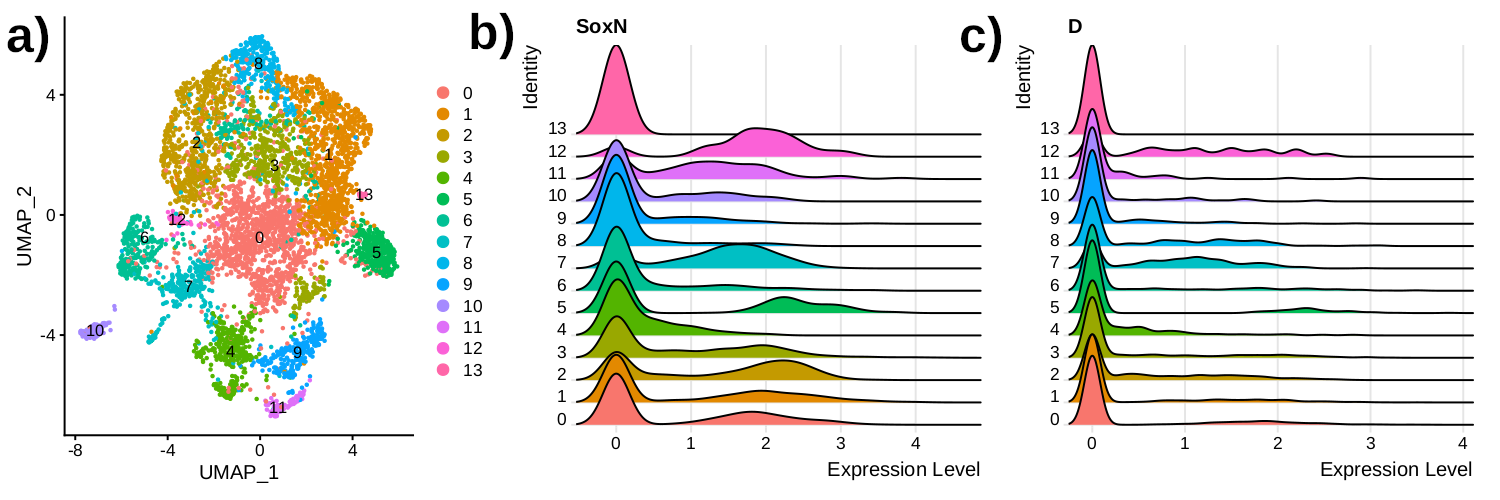
\includegraphics[width=\textwidth]{figs/Fig8 embryonic UMAP and ridges.png}
\label{fig8}
\caption{\textbf{Cell populations within the stage 6 embryo.} Data from Karaiskos \emph{et al.} was pooled to consider only the replicates from \emph{D. melanogaster}. \textbf{a)} UMAP projection was performed using the first 20 dimensions of data. Louvain clustering with 20 dimensions and a resolution parameter of 0.5 reveals 14 distinct clusters of cells, with cluster 0 containing the largest number of cells. \textbf{b-c)} Ridge plots reveal log-normalised and variance-stabilised expression of both \emph{SoxN} and \emph{D} within several clusters. \emph{SoxN} exhibits generally higher expression levels than \emph{D}, though \emph{D} shows higher expression in cluster 8. Significance testing shows that \emph{SoxN} is significantly enriched in clusters 2 and 12 while \emph{D} is enriched in clusters 5 and 12. }
\end{figure}

The UMAP projection and ridge plots for this dataset clusters into 14
total groups of cells, with clusters numbered according to the number of
cells (Figure 8a; highest cluster number has fewest cells). The ridge
plots reveal that \emph{SoxN} expression is generally higher than that
of \emph{D} (Figure 8b,c). While both genes show expression in multiple
clusters, \emph{SoxN} is only significantly enriched as a marker gene in
clusters 2 and 12 while \emph{D} is expressed weakly in cluster 5 and
significantly in cluster 12. Because both genes are coexpressed in
cluster 12, this represents an area in which both factors may share some
targets in their GRNs.

Both genes are also expressed in clusters where they are not
significantly enriched as a marker. In particular, \emph{SoxN} is
moderately expressed in clusters 0-3, 7, and 11 and weakly expressed in
clusters 4, 6, and 8-10; \emph{D} is weakly expressed in clusters 0-4,
7, 8, 9, and 11. This analysis focuses on the clusters that specifically
express \emph{SoxN} or \emph{D} as a significant marker, but
interactions are also likely in these other clusters as well. For
instance, cluster 7 contains moderate expression of both factors and its
111 genes are enriched for terms related to regulation of embryonic
development ($\sim{}$3\textsc{e}-5); cluster 8 contains higher
expression of \emph{D} than \emph{SoxN} and contains 137 genes, of which
83 (60.6\%, 8.5\textsc{e}-23) relate to anatomic structure development, 13
(9.5\%, 3.7\textsc{e}-6) relate to blastoderm segmentation, and 31 (22.6\%,
1.4\textsc{e}-31) show publication enrichment related to AP and DV patterning
\shortcite{saunders_extensive_2013}. This is consistent with a model of \emph{D}
coordinating a network of developmental processes in the tissues where
it is uniquely expressed, despite being present in low absolute
quantities.

\setcounter{figure}{9-1}
\begin{figure}[htbp]
\centering
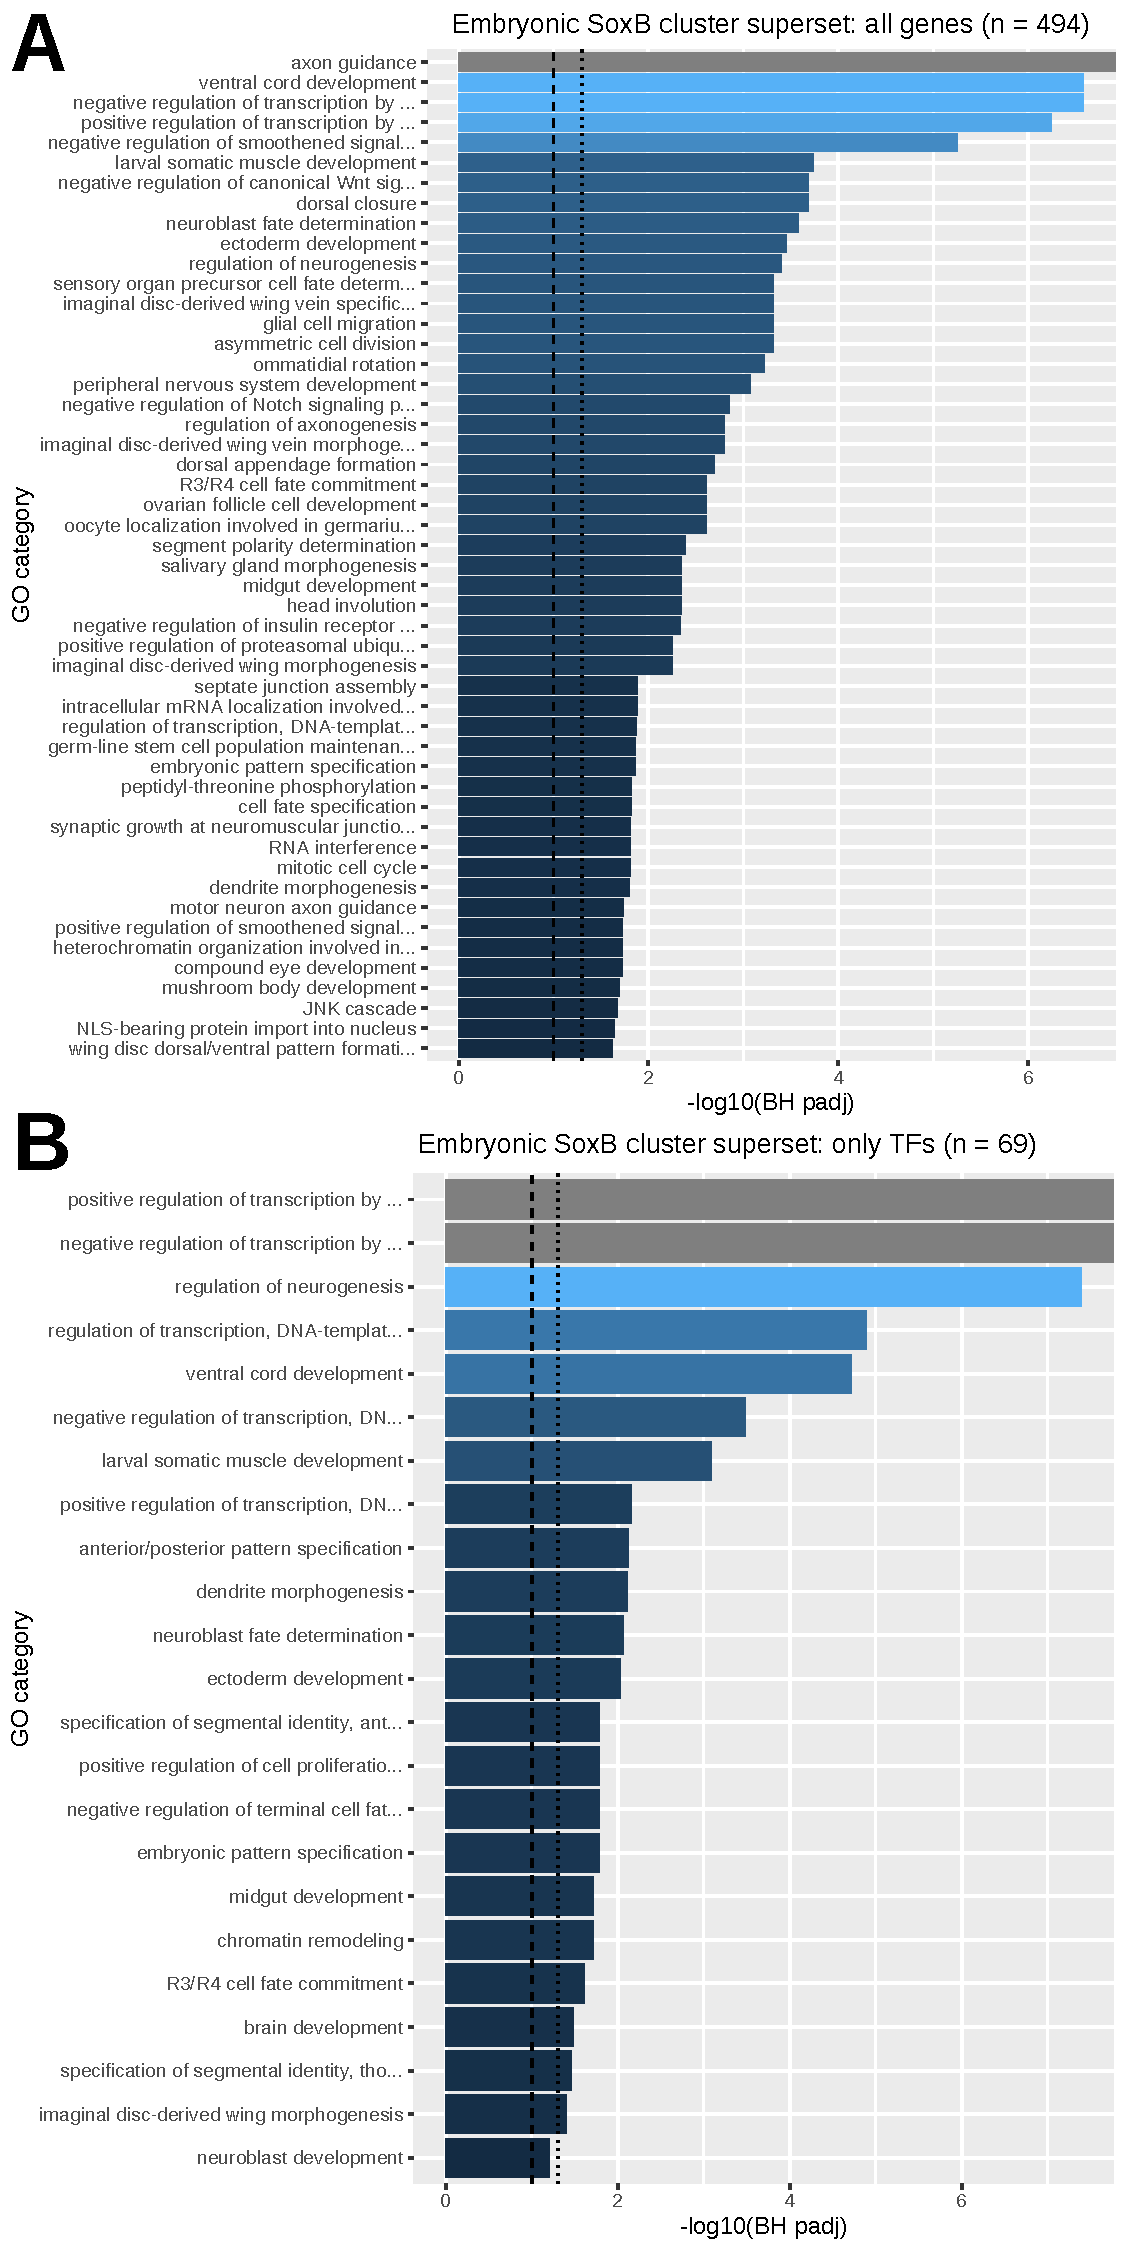
\includegraphics[height=\dimexpr\textheight-97pt\relax,keepaspectratio]{figs/Fig9 zinzen superset TF and all.pdf}
\label{fig9}
\caption{\textbf{Gene Ontology enrichment for superset of embryonic SoxB-marked clusters.} Enriched GO terms are shown along with the negative $\text{log}_{10}$ of their Benjamini-Hochberg adjusted p-values. Dashed and dotted lines signify 0.1 and 0.05 significance thresholds, respectively. Grey bars represent significant GO terms whose adjusted p-values were corrected to 0. \textbf{A)} Enrichment of all 494 annotated genes within the superset of clusters 2, 5, and 12 of the embryonic dataset. \textbf{B)} Enrichment of only the 69 annotated TFs.}
\end{figure}

\setcounter{figure}{10-1}
\begin{figure}[htbp]
\centering
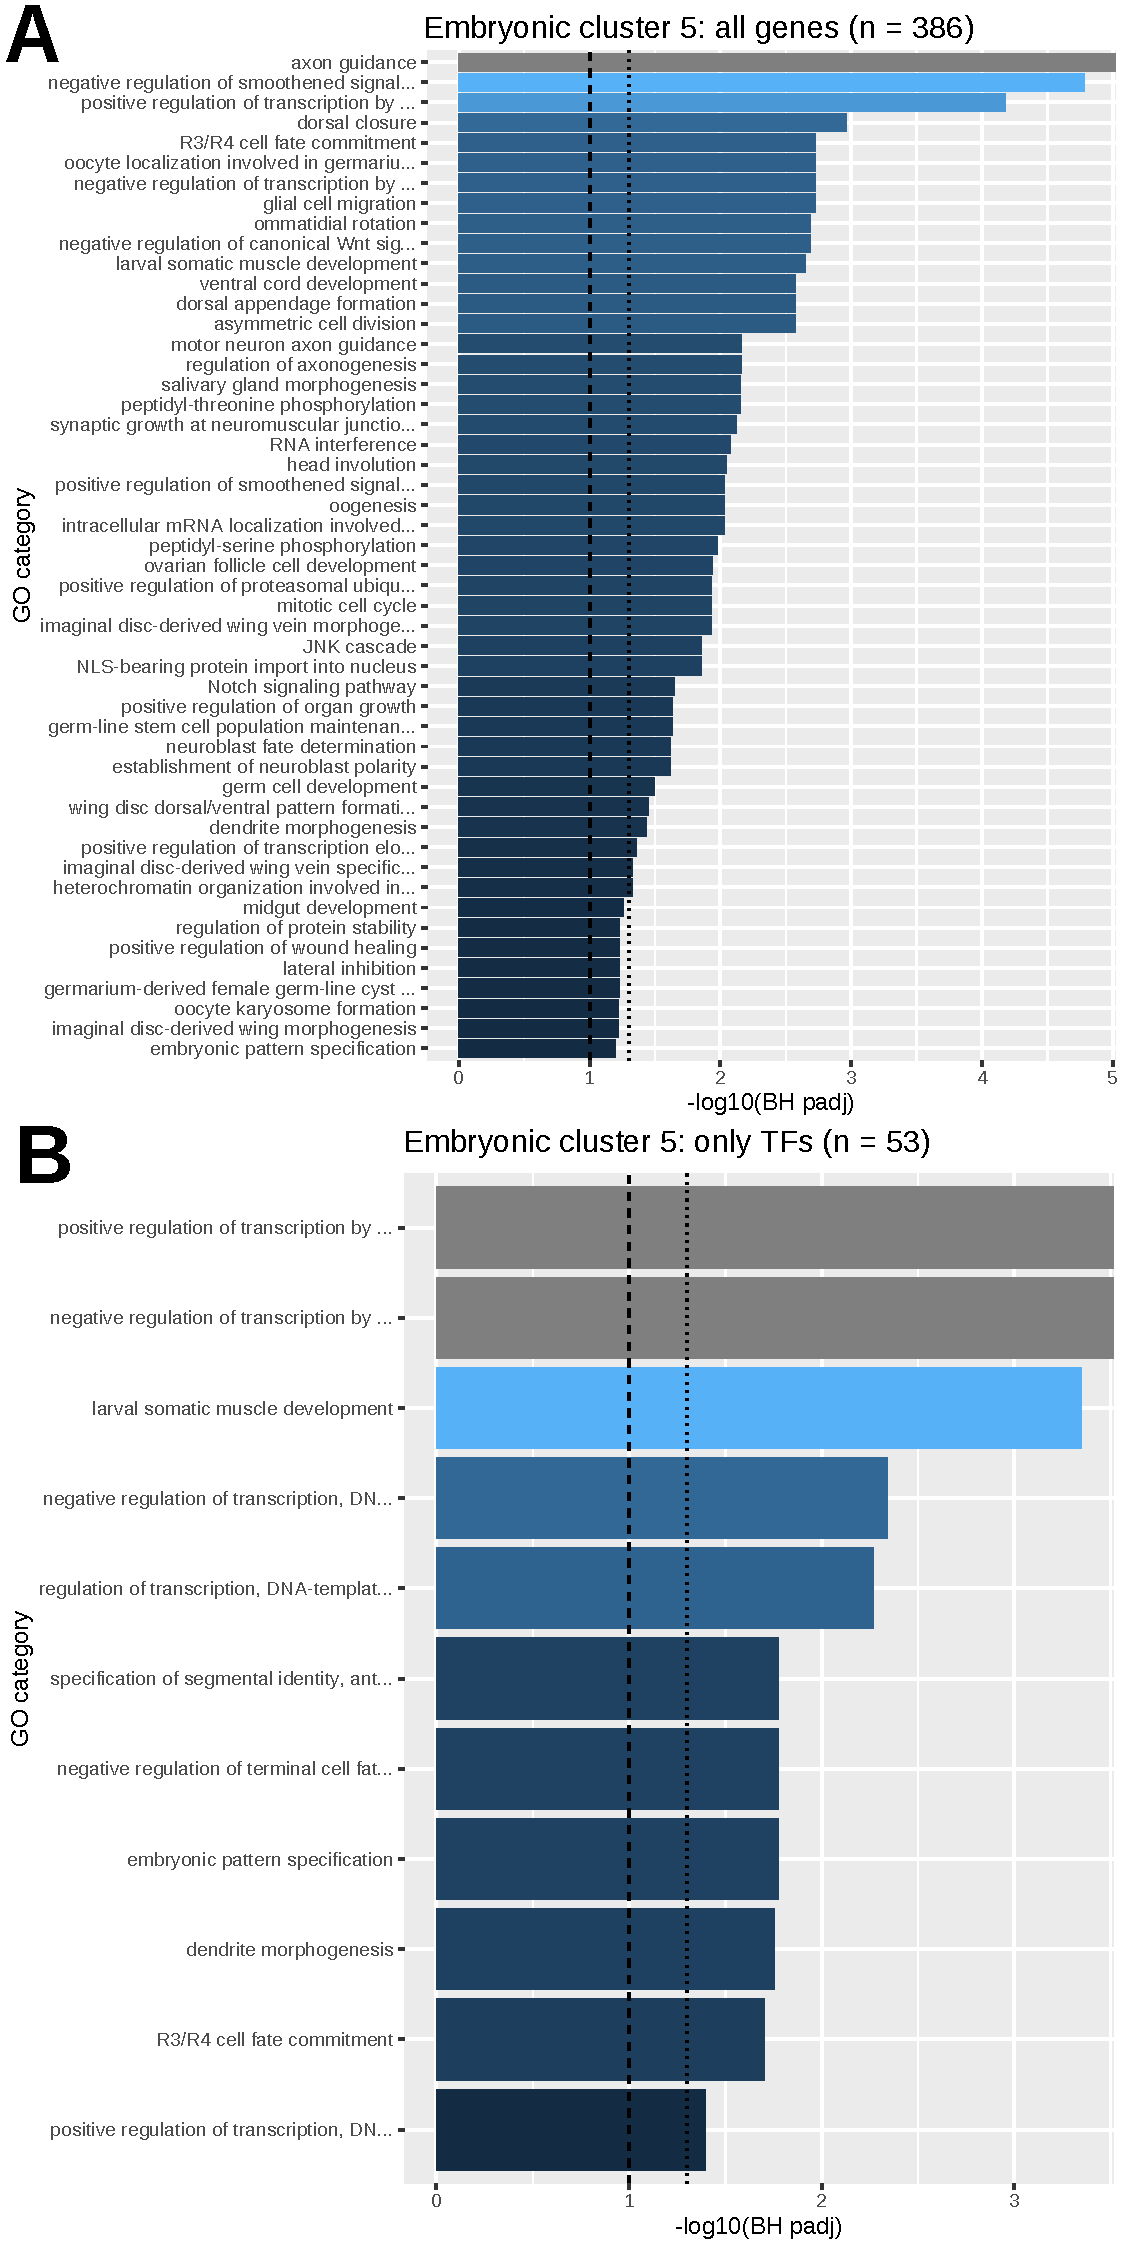
\includegraphics[height=\dimexpr\textheight-53.5pt\relax,keepaspectratio]{figs/Fig10 zinzen cluster 5.pdf}
\label{fig10}
\caption{\textbf{Gene Ontology enrichment for embryonic cluster 5.} \emph{D} is a significant marker for cluster 5 of the embryonic dataset. \textbf{A)} Enrichment plot of all 386 annotated genes within cluster 5. \textbf{B)} Enrichment of the 53 annotated TFs in the cluster.}
\end{figure}

The superset of clusters 2, 5, and 12 contains 494 genes that are
significantly enriched for several GO terms, the most significant of
which involve axon guidance, VNC development, regulation of
transcription and signalling, and neurogenesis (Figure 9a). Within this
superset, 69 of the genes represent transcription factors. The GO terms
most associated with these are unsurprisingly related to regulation of
transcription, since it is a set of TFs, but more importantly regulation
of neurogenesis, anterior/posterior patterning, and development of VNC
are all enriched terms (Figure 9b). This is consistent with the known
functions of \emph{D} and \emph{SoxN} in CNS development. Furthermore,
within the superset, 167 and 372 genes are known binding targets of
\emph{SoxN} and \emph{D} respectively \shortcite{aleksic_role_2013,ferrero_soxneuro_2014}, with 134 bound by both, reinforcing the view these are
neural cells with SoxB activity. The transcription factors in this
superset therefore appear to play more of a regulatory role than the
other genes, indicating that the biological processes driven by the full
superset gene list may largely be a result of genes that are targets of
these TFs.

Within cluster 2, there are 44 markers and these show weak enrichment
for genes involved in negative regulation of Notch signalling and
myoblast migration . This cluster contains 5 genes annotated as TFs,
including \emph{SoxN}, \emph{opa}, \emph{odd}, \emph{tsh}, \emph{pnr},
and \emph{gsb}. Analysis of these genes in FlyMine \shortcite{lyne_flymine_2007}
reveals that these genes are primarily related to patterning and
segmentation. Indeed, \emph{opa} is known to show a conserved
interaction with with \emph{D} during insect segmentation \shortcite{clark_evidence_2018} and later in the larval CNS it functions as a negative
regulator of \emph{D} to push neural stem cells toward their later
stages of differentiation \shortcite{abdusselamoglu_transcription_2019}. This may imply
that lack of significant \emph{D} expression in this cluster is
consistent with a mechanism in which \emph{SoxN} but not \emph{D} helps
cells progress to a post-neuroblast state \shortcite{ferrero_soxneuro_2014}.
Downregulation of Notch signalling is also known to correspond to
transition from progenitor cells to neuroblasts \shortcite{contreras_dynamic_2018}, further supporting the idea that cluster 2 represents a
relatively large group of cells that includes neuroblasts.

Cluster 5 contains 423 genes, which show a significant enrichment for
neural functions and various terms related to developmental processes,
including Smo and Wnt signalling pathways. Almost 70\% of the genes in
this cluster are annotated with the high level GO term ``regulation of
biological processes'', suggesting actively differentiating cells.
Analysis of BDGP expression via FlyMine \shortcite{hammonds_spatial_2013,lyne_flymine_2007,tomancak_systematic_2002,tomancak_global_2007} shows strong enrichment for
expression in the ventral ectoderm (5.0\textsc{e}-17), procephalic ectoderm
(1.7\textsc{e}-12), and VNC primordium (2.8\textsc{e}-12), consistent with SoxB expression
in the neuroectoderm. In this cluster 53 genes (12.5\%) are
transcription factors with weak enrichment for embryonic patterning and
dendrite morphogenesis (Figure 10).

While \emph{Dichaete} is only weakly enriched in this cluster, 277
(65.5\%) of these genes are known to be bound by \emph{D}, indicating
that even weak \emph{D} presence may indicate a central coordinating
role within the GRN. Additionally, while the cluster 5 TFs were enriched
for a few distinct processes such as segment specification and muscle
development, the full cluster 5 gene list is enriched for various other
functions such as R3/R4 photoreceptor fate commitment, glial cell
migration, neuromuscular junction growth, axon guidance, JNK signalling,
and oogenesis. This points to a role in which \emph{Dichaete} serves as
a regulatory hub \shortcite{aleksic_role_2013} that coordinates a wider set of
genes during the process of segmentation, CNS specification and
differentiation. Simultaneously, FlyMine localisation analysis shows
that many of the TFs in this category, such as the aforementioned
\emph{opa,} are known to be active in the developing VNC and ventral
ectoderm. This suggests that \emph{D} may be acting in conjunction with
other TFs in this cluster to coordinate a wide range of developmental
processes related to patterning and differentiation.

Cluster 12 is much smaller than the other clusters, but is the only one
that exhibits strong \emph{SoxN} and \emph{D} expression. The cluster
contains 92 genes enriched for expression in the procephalic and ventral
ectoderm ($\sim{}$2\textsc{e}-14 each), of which 13 (14.1\%) are
annotated as TFs (Figure 11). Of particular interest is the fact that
several of these genes are E(spl) helix-loop-helix (HLH) and Bearded
family members, indicating a connection between genes in this cluster
and the Notch signalling pathway \shortcite{dearden_origin_2015,lai_enhancer_2000}. The
interaction between Bearded members and the E3 ligase \emph{Neuralised}
(\emph{Neur}), which was also present in the cluster, is known to
spatially regulate \emph{Delta} signalling to promote neurogenesis
\shortcite{bardin_bearded_2006}. It is therefore plausible that
\emph{SoxN} and \emph{D} coordinate with other neurodevelopmental genes
in the cluster, such as \emph{vnd} and \emph{l'sc}, to regulate the
signalling pathways that contribute to neuroblast delamination and
specification into neurons.

\setcounter{figure}{11-1}
\begin{figure}[htbp]
\centering
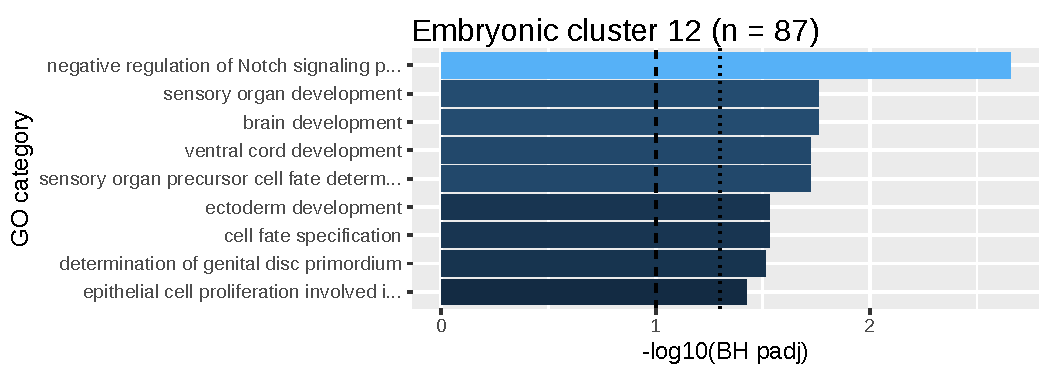
\includegraphics[width=\dimexpr\textwidth\relax,keepaspectratio]{figs/Fig11 zinzen cluster12.pdf}
\label{fig11}
\caption{\textbf{Gene Ontology enrichment for embryonic cluster 12.} \emph{SoxN} and \emph{D} are both significant markers for cluster 12 of the embryonic dataset, which contains GO annotations for 87 genes.}
\end{figure}

In summary, the SoxB-focused analysis of scRNA-seq data from the
blastoderm/early gastrulating embryo reveals clusters of cells involved
in early aspects of neural development as well as some more specific
annotations that may indicate \emph{D} or \emph{SoxN} exclusive
functions. Since the expression of \emph{D} and \emph{SoxN} in the early
embryo have been well characterised, the analysis of this dataset offers
confidence in extending this approach to the larval brain and adult VNC
datasets.

\subsection{Larval Brain Dataset}

The dataset from Avalos \emph{et al}. examines the first instar larval
brain dissected away from the ventral nerve cord and is therefore
expected to contain more cells and genes that relate specifically to
neurodevelopment. The cells cluster into 19 distinct groups (Figure
12a), with \emph{SoxN} highly expressed in several groups and \emph{D}
moderately expressed across most clusters (Figure 12b). \emph{SoxN} is
significantly expressed as a marker gene in clusters 6, 7, 8, and 10,
while \emph{D} is not significantly enriched as a marker for any
individual cluster, although some expression of both \emph{D} and
\emph{SoxN} is seen in cluster 13. Therefore, the bulk of analysis in
this dataset focuses on the clusters where \emph{SoxN} is identified as
a marker. Notably, clusters 6, 7, 8, 10, and 13 are closely related on
the UMAP projection.

\setcounter{figure}{12-1}
\begin{figure}[bhtp]
\centering
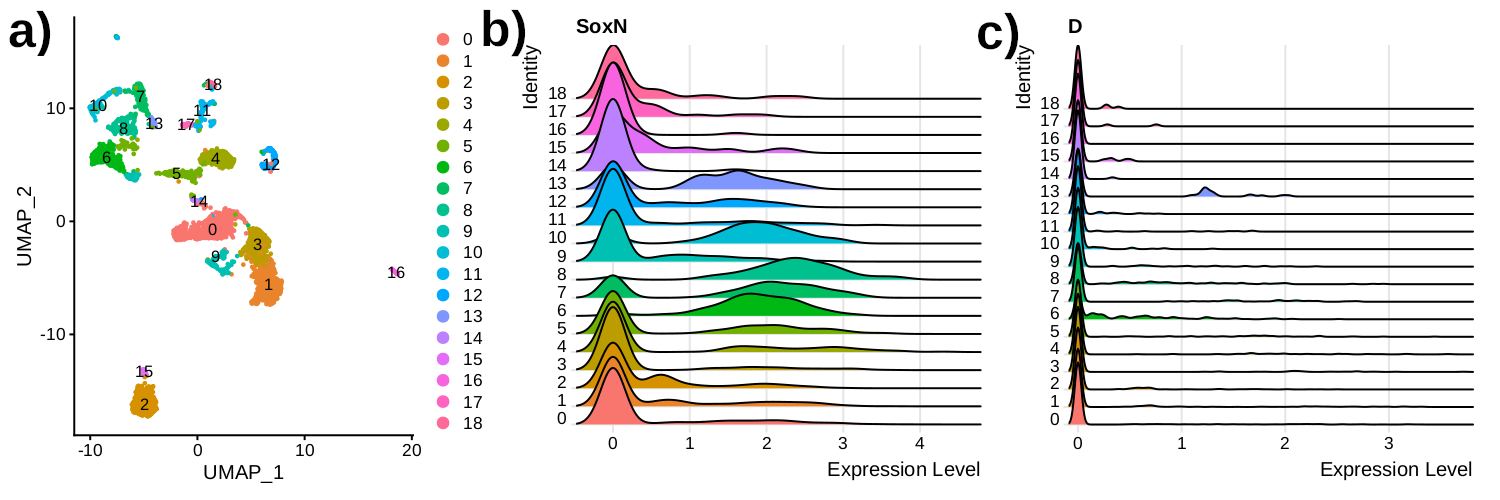
\includegraphics[width=\textwidth]{figs/Fig12 larval UMAP and ridges.png}
\label{fig12}
\caption{\textbf{Cell populations within the first instar larval brain.} Data from Avalos \emph{et al.} was filtered to keep only unstarved wild-type replicates. \textbf{a)} UMAP projection used the first 20 dimensions of data. Louvain clustering with the first 20 dimensions and a resolution parameter of 0.5 results in 19 distinct clusters of cells. \textbf{b-c)} Ridge plots show log-normalised expression of \emph{SoxN} and \emph{D}. \emph{SoxN} shows moderate expression in several clusters, and is significantly enriched in clusters 6, 7, 8, and 10. Notably, cluster 13 appears related to these clusters in this projection. While \emph{D} displays a lower baseline level of expression and is not significantly enriched within any cluster, there is some expression in clusters 6 and 13.}
\end{figure}


\setcounter{figure}{13-1}
\begin{figure}[htbp]
\centering
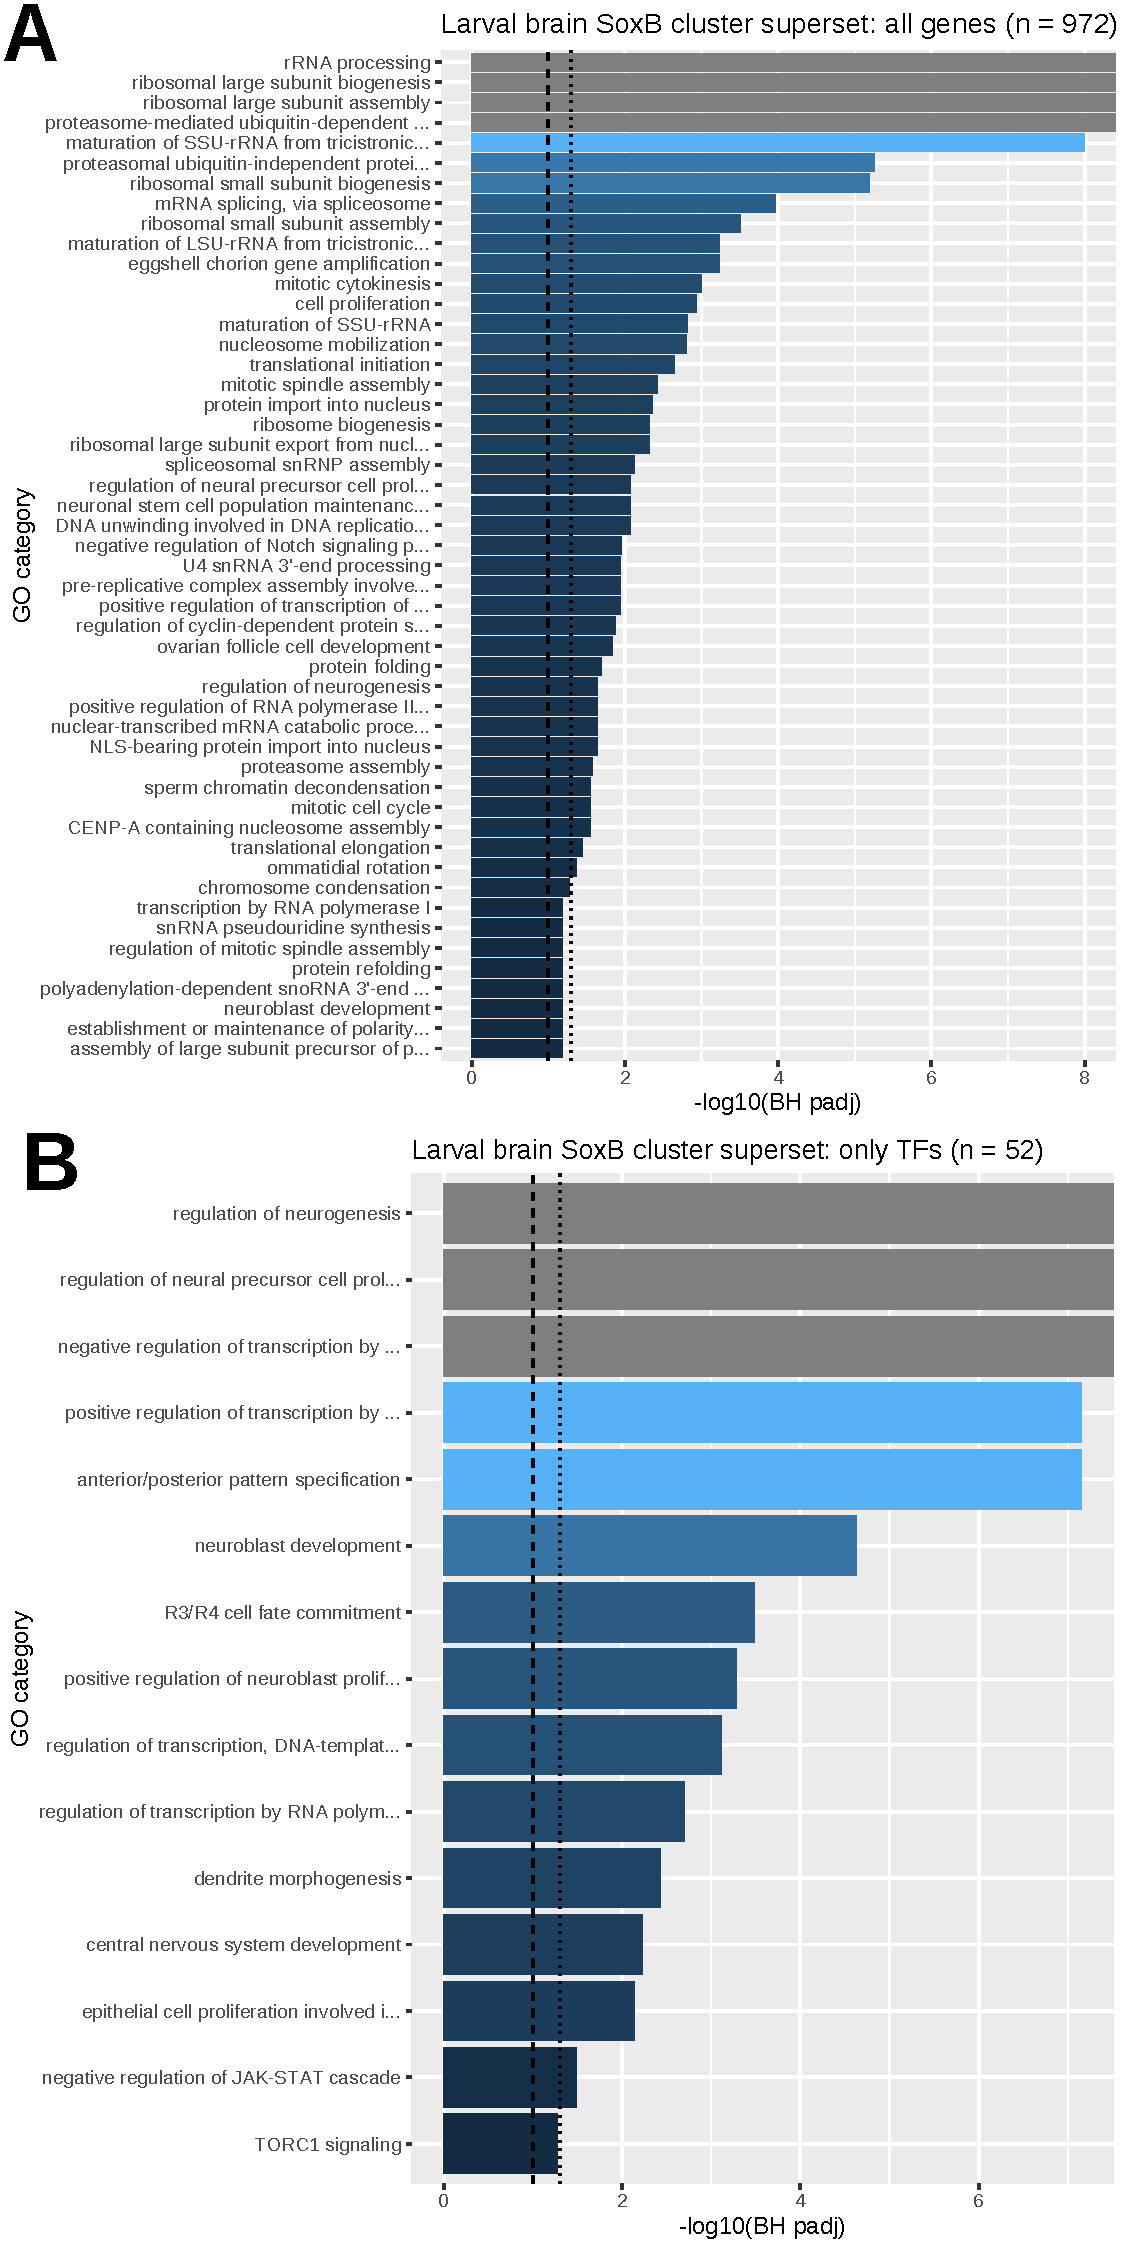
\includegraphics[height=\dimexpr\textheight-68pt\relax,keepaspectratio]{figs/Fig13 avalos superset.pdf}
\label{fig13}
\caption{\textbf{Gene Ontology enrichment for superset of larval brain SoxB-marked clusters.} This superset includes clusters 6, 7, 8, and 10. All of these clusters feature \emph{SoxN} as a marker while none include \emph{D}. \textbf{A)} Enrichment plot of all 972 annotated genes within this superset. \textbf{B)} Enrichment plot of the 52 annotated TFs in the superset.}
\end{figure}

The superset of clusters 6, 7, 8, and 10 contains a large number
(\emph{n} $=$ 972) of translation-related gene ontologies, as well as
annotations for mRNA processing, ubiquitin proteasome activity, and cell
proliferation (Figure 13a). In contrast, restricting the list to only
the 52 TFs within the superset reveals that the primary annotations are
for regulation of neurogenesis, anterior/posterior patterning,
neuroblast development, and other nervous system related terms (Figure
13b). Examining only the SoxN bound targets within the superset shows
strong enrichment for cytoplasmic translation (\emph{p} \textless{}
3\textsc{e}-5), neural precursor development (\emph{p} \textless{} 1.8\textsc{e}-4), and
regulation of Notch signalling (\emph{p} \textless{} 1.8\textsc{e}-4) as well as
eye-antennal disc morphogenesis (\emph{p} \textless{} 3.2\textsc{e}-3) that is
influenced by anterior/posterior patterning \shortcite{morata_development_1979}
and is a site of \emph{SoxN} expression \shortcite{cremazy_genome-wide_2001}. While
\emph{Dichaete} but not \emph{SoxN} is associated with
anterior/posterior patterning in the embryo, many of the proteins
involved in early segmentation are subsequently used in CNS patterning.
This may suggest that patterning genes can be regulated by both the SoxB
proteins, as might be expected from their extensive binding overlap in
the embryo \shortcite{ferrero_soxneuro_2014}, and that neural-specific regulation
is simply a reflection of restricted SoxB expression. In addition, it is
possible that these data are also consistent with a model in which
\emph{D} works with \emph{SoxN} early in development to regulate
transcriptional and translational processes for neurogenesis. It is also
possible that the lack of significant \emph{D} expression in the first
instar is consistent with data that show \emph{D} expression highly
restricted in larval neuroblasts as part of a temporal cascade activated
in third instar larva that controls neural identify \shortcite{apitz_region-specific_2015,suzuki_temporal_2013}.

\setcounter{figure}{14-1}
\begin{figure}[htbp]
\centering
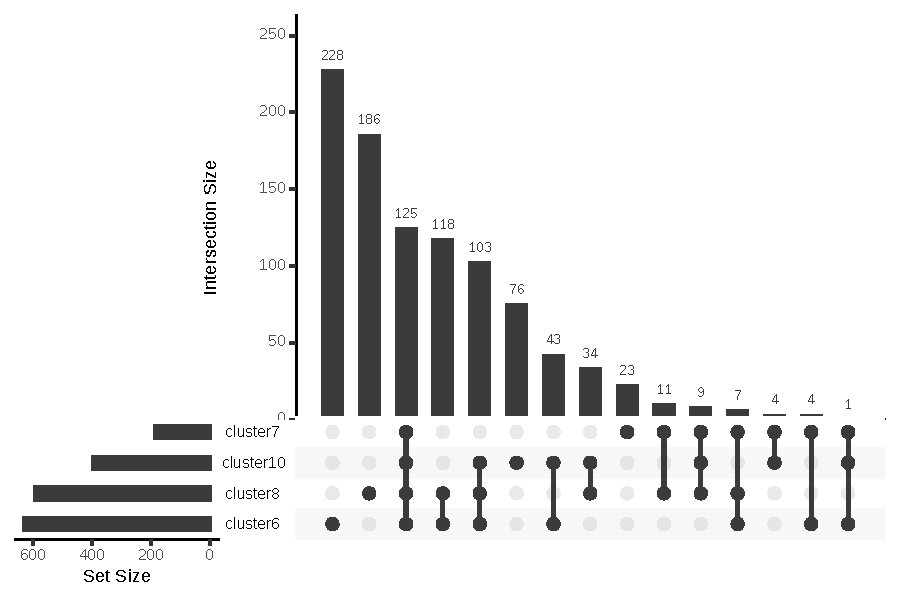
\includegraphics[width=\textwidth]{figs/Fig14 Avalos Upset.pdf}
\label{fig14}
\caption{\textbf{UpSet plot of larval brain dataset clusters.} \emph{SoxN}-positive clusters share many of the same marker genes, and UpSet representation can visualise the size of each intersection set. Clusters 6, 7, 8, and 10 bear a high degree of resemblance in terms of their expressed markers: 125 genes are shared by all four clusters, while 118 are shared by clusters 6 and 8. Overlap in these gene lists may indicate the presence of shared network elements that relate to \emph{SoxN} and \emph{D} regulation.\vspace{0.5cm}}
\end{figure}

\setcounter{figure}{15-1}
\begin{figure}[htbp]
\centering
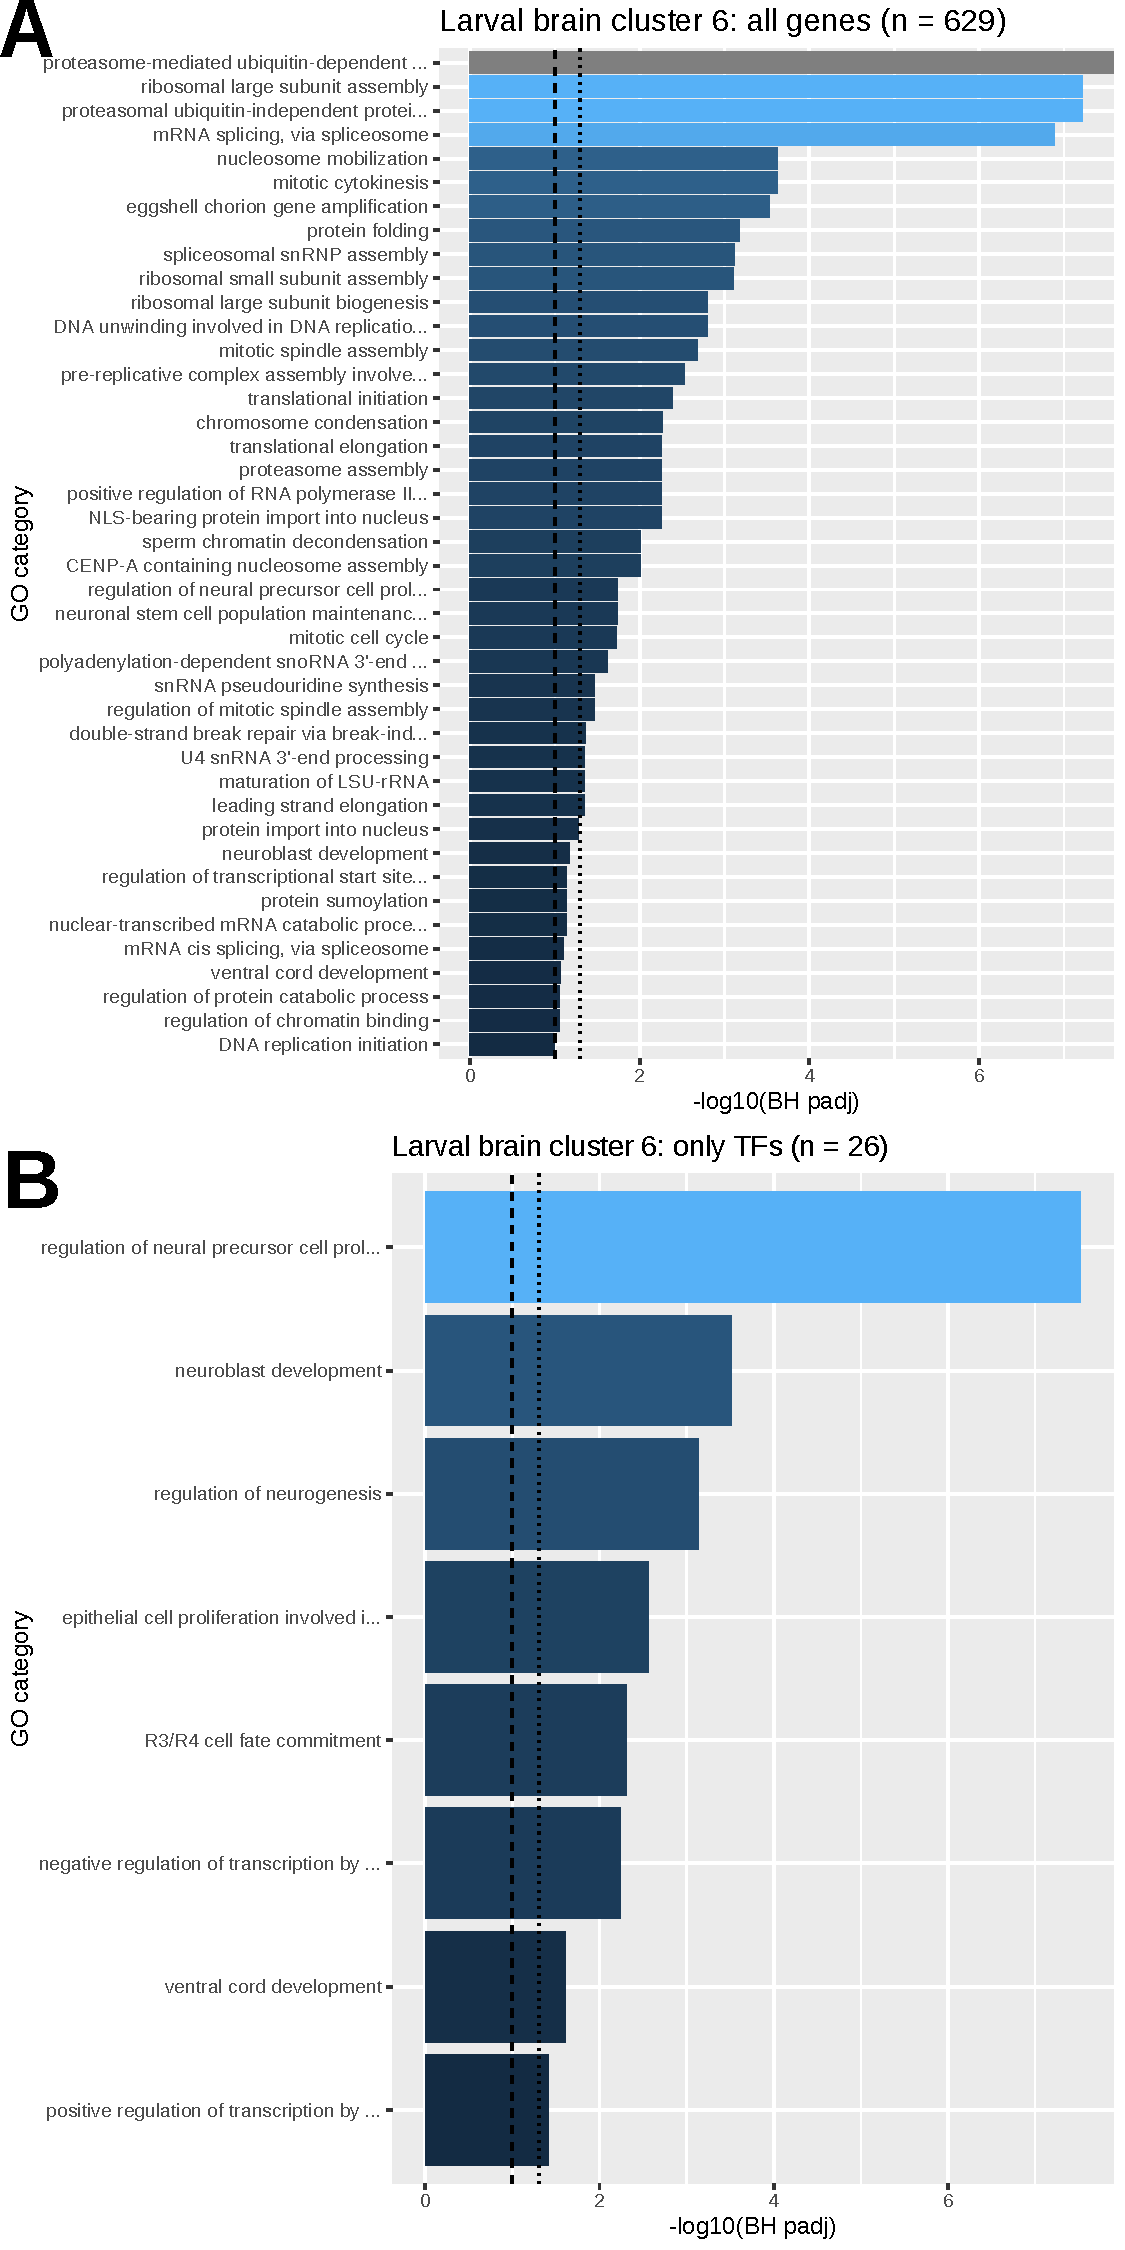
\includegraphics[height=\dimexpr\textheight-53.5pt\relax,keepaspectratio]{figs/Fig15 avalos cluster 6.pdf}
\label{fig15}
\caption{\textbf{Gene Ontology enrichment for larval brain cluster 6.} \emph{SoxN} is a significant marker for cluster 6 of the larval brain dataset. \textbf{A)} Enrichment plot of all 629 annotated genes within cluster 6. \textbf{B)} Enrichment of the 26 annotated TFs in the cluster.}
\end{figure}

The original paper by Avalos \emph{et al.} used an alternative
computational approach to generate 29 different cell clusters, each
corresponding to particular cell type annotations \shortcite{brunet_avalos_single_2019}. Of these clusters, only one expresses \emph{SoxN} as a marker
gene and is annotated as ``neural progenitor cells 2.'' A total of 6
clusters from the original paper are annotated as corresponding to NPCs,
all of which received their categorisation based on literature-based
annotations. Within this cluster, other marker genes include \emph{sna},
\emph{klu}, \emph{fru}, and \emph{cas}; all four of which are
co-expressed with \emph{SoxN} in clusters 6, 7, and 8 in my analysis,
indicating that the three clusters in this categorisation may be related
to ``neural progenitor cells 2'' from the original paper. However, while
all of these factors are markers for clusters 6 through 8, all of them
except \emph{sna} and \emph{SoxN} are also expressed in cluster 13, and
each gene is also uniquely expressed in some other clusters. While there
is not an exact correspondence between clusters from the two analyses,
this provides a starting assumption that \emph{SoxN}-positive cells in
clusters 6, 7, and 8 will generally behave similarly to NPCs. While none
of these factors appear to be shared in cluster 10, UpSet analysis of
the \emph{SoxN}-positive clusters reveals that while only 7 genes are
shared uniquely between clusters 6 through 8, 125 genes are shared
between clusters 6, 7, 8, and 10, suggesting that cluster 10 of this
analysis may also be NPC-related (Figure 14).


\setcounter{figure}{16-1}
\begin{figure}[htbp]
\centering
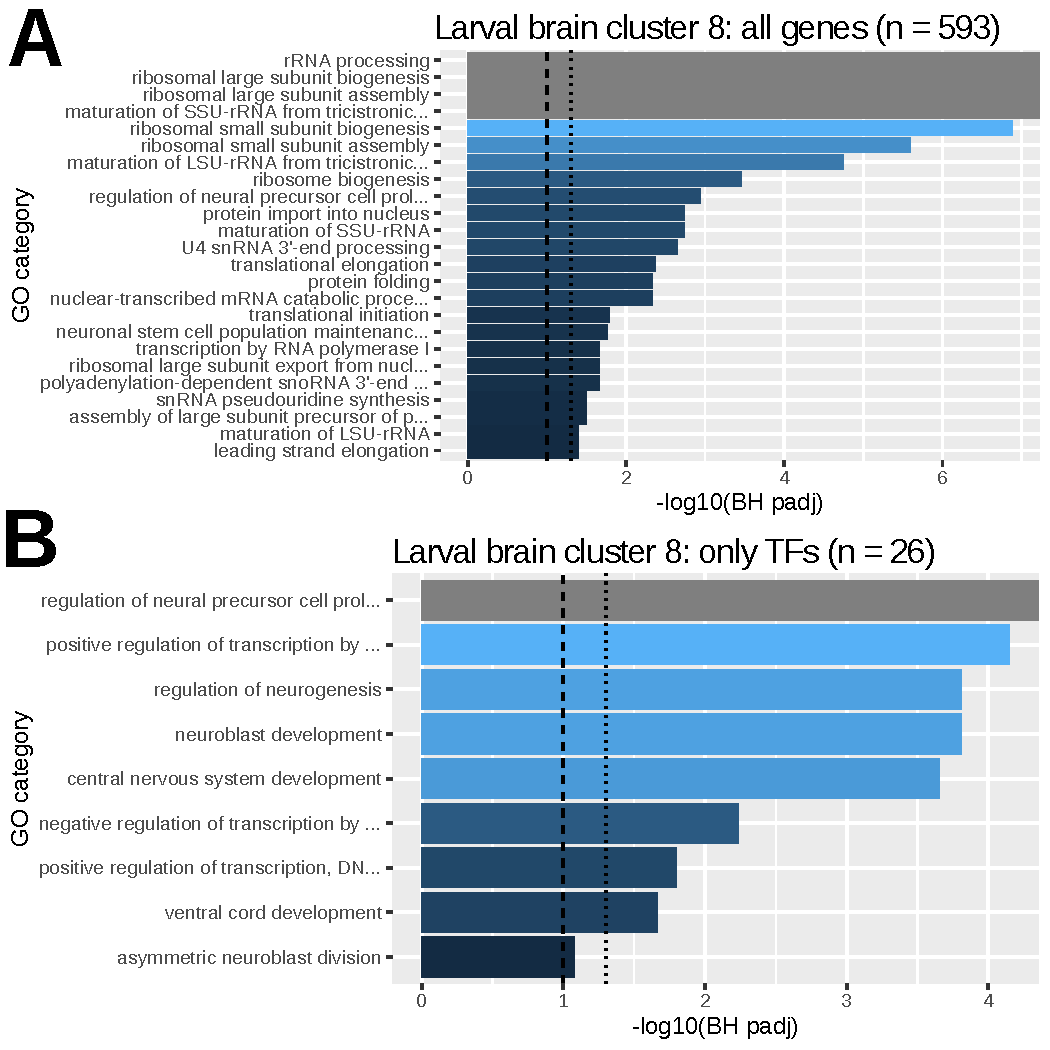
\includegraphics[width=\textwidth,keepaspectratio]{figs/Fig16 avalos cluster8.pdf}
\label{fig16}
\caption{\textbf{Gene Ontology enrichment for larval brain cluster 8.} \emph{SoxN} is a significant marker for cluster 8 of the larval brain dataset. \textbf{A)} Enrichment plot of all 593 annotated genes within cluster 8. \textbf{B)} Enrichment of the 26 annotated TFs in the cluster.}
\end{figure}

\setcounter{figure}{17-1}
\begin{figure}[htbp]
\centering
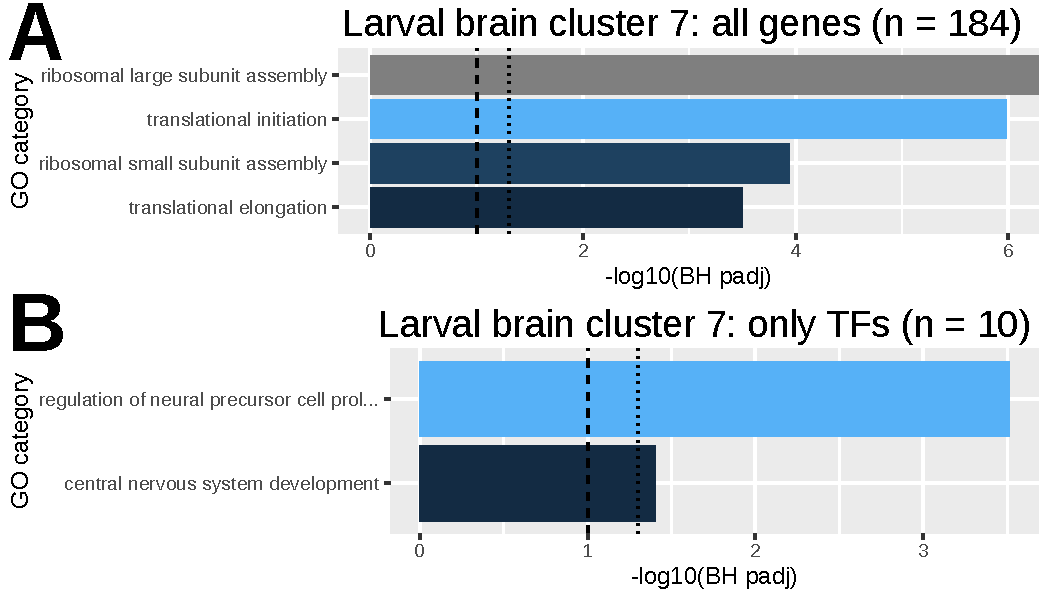
\includegraphics[width=\dimexpr\textwidth\relax,keepaspectratio]{figs/Fig17 avalos cluster7.pdf}
\label{fig17}
\caption{\textbf{Gene Ontology enrichment for larval brain cluster 7.} \emph{SoxN} is a significant marker for cluster 7 of the larval brain dataset. \textbf{A)} Enrichment plot of all 184 annotated genes within cluster 7. \textbf{B)} Enrichment of the 26 annotated TFs in the cluster.}
\end{figure}

\setcounter{figure}{18-1}
\begin{figure}[htbp]
\centering
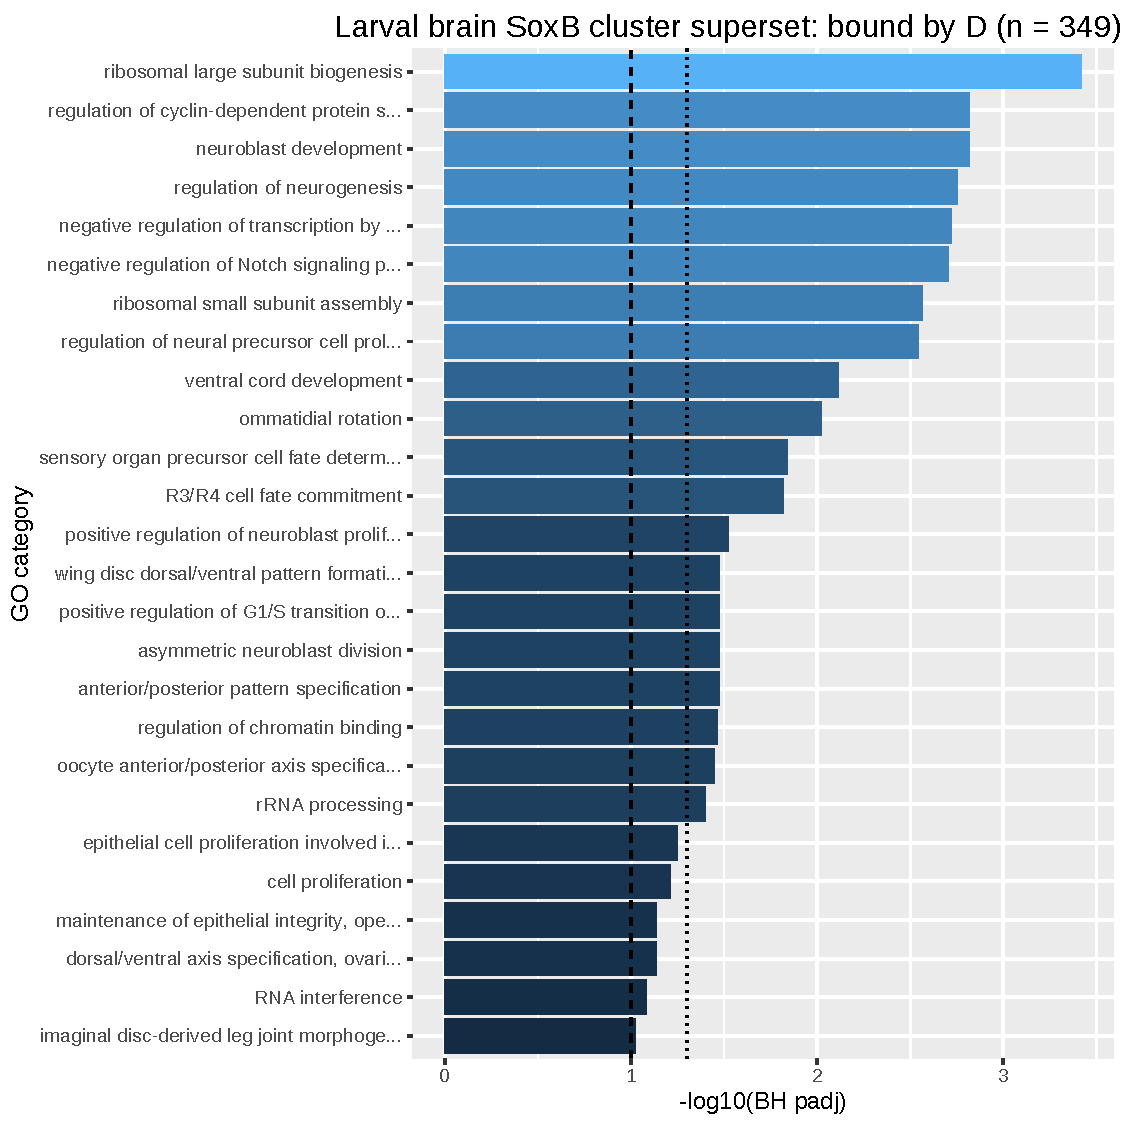
\includegraphics[width=\dimexpr\textwidth\relax,keepaspectratio]{figs/Fig18 avalos Combined_clusterSuperset_DBind.pdf}
\label{fig18}
\caption{\textbf{Gene Ontology enrichment for D-bound genes within superset of larval brain SoxB-marked clusters.} 35.9\% of genes in the superset of markers for clusters 6, 7, 8, and 10 (Figure 13a) are bound by Dichaete in the embryo \protect\shortcite{aleksic_role_2013}.}
\end{figure}

Despite the similarities between these clusters, there still appear to
be marked differences. The neural marker \emph{Dpn} is present in
clusters 6 and 8 but not 7 or 10. Within cluster 6, only 26 (4.1\%) of
the 629 identified markers are annotated as transcription factors.
Within the full set, the most enriched GO terms involve mRNA processing,
proteasome degradation, and translation, but within only the TFs,
neuroblast development and regulation of neurogenesis are the most
significant processes (Figure 15). This, along with general CNS
development, is also true of cluster 8 (Figure 16), which shares a full
16 of the 26 TFs and 353 of the same cluster markers as cluster 6.
Cluster 6 possesses marker genes such as \emph{sna}, \emph{wor}, and
\emph{ase} that suggest neuroblast selection and delamination \shortcite{arefin_drosophila_2019}. Both clusters share a large number of ribosomal genes
related to translation, and interestingly, both contain over 200 genes
annotated as \emph{D} bound targets. Despite not expressing \emph{D} as
a marker, this is consistent with an interpretation of clusters 6 and 8
as neuroblasts that have not yet initiated \emph{D} expression but that
have a Dichaete-regulated GRN ready for temporal activation.

Cluster 7 is similar to clusters 6 and 8, but is more highly dominated
by ribosomal and translational genes; considering only the 10 TFs in
this cluster yields high GO enrichment for CNS development and NPC
proliferation (Figure 17). Because these TFs include \emph{SoxN} and the
shared \emph{sna}, \emph{klu}, \emph{fru}, and \emph{cas}, it is
possible that cluster 7 represents a subgroup of neuroblasts that are
actively promoting translation as they commit to becoming neurons. While
fewer of the genes in cluster 7 are binding targets for \emph{D} as
compared to clusters 6 and 8, 36 of the 65 targets come from ribosomal
genes; indeed, both the superset and intersection set of clusters 6, 7,
8, and 10 are enriched for ribosomal assembly processes when considering
only \emph{D} binding targets (Figure 18). While \emph{D} is not a
marker in any of these putative neuroblast clusters, it still has
moderate baseline expression within these cells and may direct networks
related to translation and neuroblast commitment once the temporal
cascade activates its expression.

\setcounter{figure}{19-1}
\begin{figure}[htb]
\centering
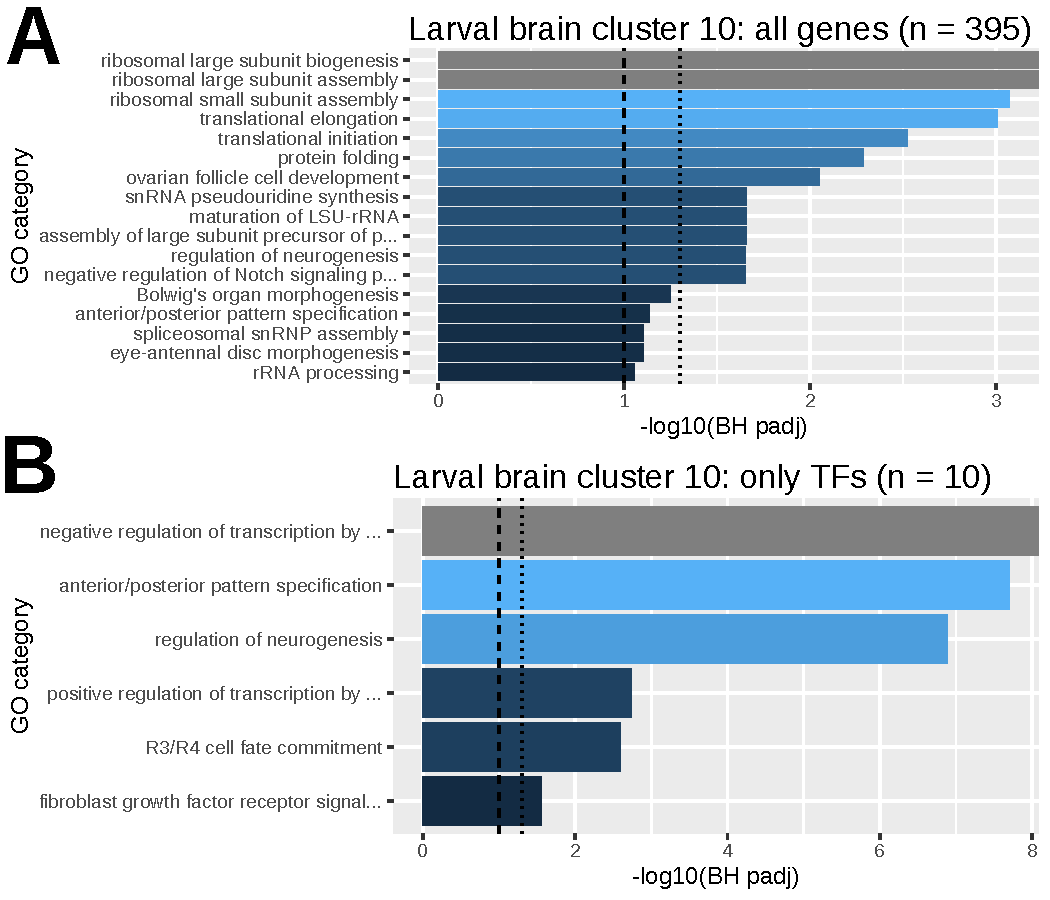
\includegraphics[width=\dimexpr.75\textwidth\relax,keepaspectratio]{figs/Fig19 avalos cluster10.pdf}
\label{fig19}
\caption{\textbf{Gene Ontology enrichment for larval brain cluster 10.} \emph{SoxN} is a significant marker for cluster 10 of the larval brain dataset. \textbf{A)} Enrichment plot of all 395 annotated genes within cluster 10. \textbf{B)} Enrichment of the 20 annotated TFs in the cluster.}
\end{figure}

While the UpSet analysis (Figure 14) shows that cluster 10 shares
similarities with clusters 6 through 8, it does not share the core
markers defined by Avalos \emph{et al}. Though its full GO enrichment is
dominated by processes related to ribosomal assembly, its 20
transcription factors are enriched for negative regulation of
transcription, anterior/posterior patterning, and neurogenesis (Figure
19). This cluster expresses \emph{Tll}, the final element after \emph{D}
in the temporal cascade that determines the neural progeny of
neuroblasts \shortcite{li_temporal_2013}. It is therefore possible that cluster
10 represents a version of the cells in clusters 6 through 8 that are in
the process of committing to neuronal fate or have already committed.

Taken together, my analysis of the larval brain scRNA-seq data reveals
clusters of neural cells that appear to be highly translationally
active. The absence of genes encoding neurotransmitters, which are
present in several of the clusters that do not express SoxB, indicates
that SoxB expressing cells are all neuroblasts or progenitors, a
suggestion supported by enrichment for cell-cycle related genes. In
keeping with the mapped expression in the larval CNS, \emph{SoxN} shows
much greater enrichment than \emph{Dichaete}, the latter being expressed
in a highly restricted pattern in the developing optic lobes.

\setcounter{figure}{20-1}
\begin{figure}[htbp]
\centering
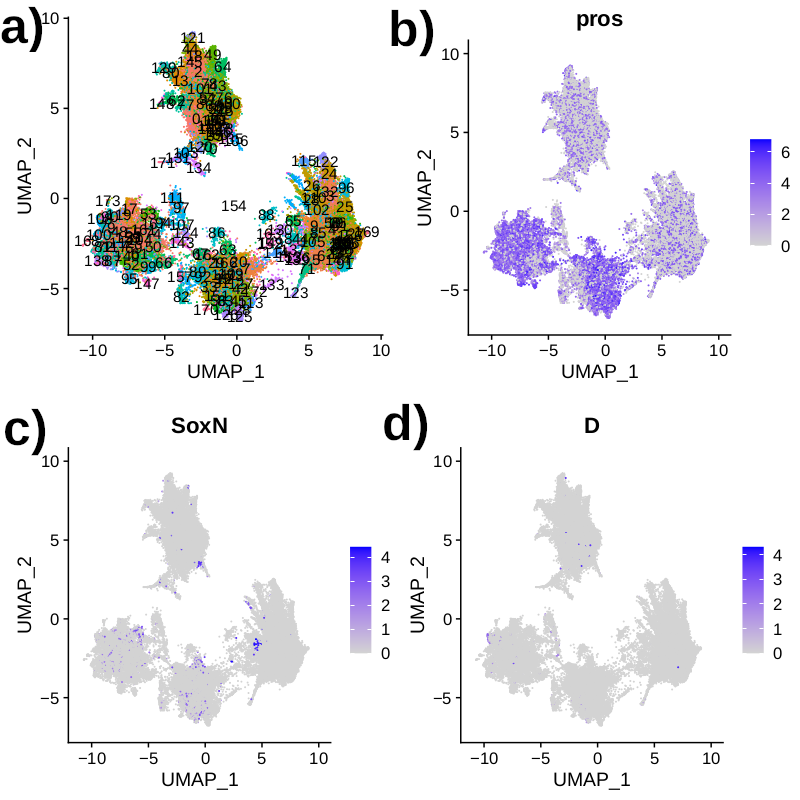
\includegraphics[width=\textwidth]{figs/Fig20 adult brain UMAP and features.png}
\label{fig20}
\caption{\textbf{Cell populations within the adult ventral nerve cord.} Male replicates from Allen \emph{et al.} were pooled and processed on the Rustbucket server. \textbf{a)} UMAP projection used the first 45 dimensions, and Louvain clustering used the first 45 dimensions with a resolution parameter of 12 to produce 174 total cell clusters. \textbf{b-d)} Relative log-normalised expression levels of the neuroblast/GMC marker \emph{pros} as well as of \emph{SoxN} and \emph{D} are shown on the original projection. While \emph{pros} exhibits expression over a wide range of cell clusters, \emph{SoxB} expression is more limited, with \emph{SoxN} more highly expressed than \emph{D}. Significance testing shows \emph{SoxN} enriched in clusters  53, 108, 126, 135, 140, 151, 159, and 167, with \emph{D} enriched in cluster 108 as well.}
\end{figure}

\subsection{Adult Ventral Nerve Cord Dataset}

The dataset from Allen \emph{et al.} is derived from the dissected adult
ventral nerve cord, and sampled by far the greatest number of cells
($\sim{}$26,000) of the 3 analyses. My UMAP analysis identified
174 distinct cell clusters (Figure 20a). This was the only dataset
processed with dimensions 1 through 45 and with a cluster resolution of
12, as the original paper reveals that there is significant information
far beyond the first 20 dimensions \shortcite{allen_single-cell_2020}. Projecting
\emph{SoxN}, \emph{D} and the neuroblast/GMC marker \emph{Prospero} \shortcite{li_pan-neural_2000} into
these UMAP plots revealed widespread \emph{pros} expression in many
clusters, reflecting a high proportion of neuroblast and post-neuroblast
lineages (Figure 20b). In contrast, \emph{SoxN} and \emph{D} are far
more restricted in their expression, with \emph{Dichaete} in particular
limited to very few clusters. (Figure 20c-d).
Within these defined clusters, \emph{SoxN} is a marker for clusters 53,
108, 126, 135, 140, 151, 159, and 167, while \emph{D} is a marker only
in cluster 108. Overall, \emph{SoxN} is expressed in 2.5\% of the cells
in the dataset while \emph{D} is expressed in only 0.4\%.

In cluster 108, \emph{D} is present in 63.7\% of cells and \emph{SoxN}
in 40.9\%. The cluster is enriched for neuronal-related GO terms, in
particular synaptic functions, suggesting these are post-mitotic cells.
The cluster is enriched for genes expressed in the embryonic brain (140
genes, 4.6\textsc{e}-16) with 40\% (220 genes) bound by Dichaete in the embryo.
Of the 34 TFs in this cluster, 24 are expressed in the embryonic brain
and 11 of these have annotated roles in neuron development (3.5\textsc{e}-5),
reinforcing the view that this cluster represents differentiating
neurons. (Figure 21). Interestingly, this cluster also expresses
\emph{Sox21b}, which exhibits CNS expression in the
late embryo and larva and is likely co-regulated with \emph{Dichaete}
\shortcite{mckimmie_conserved_2005}.

\setcounter{figure}{21-1}
\begin{figure}[htb]
\centering
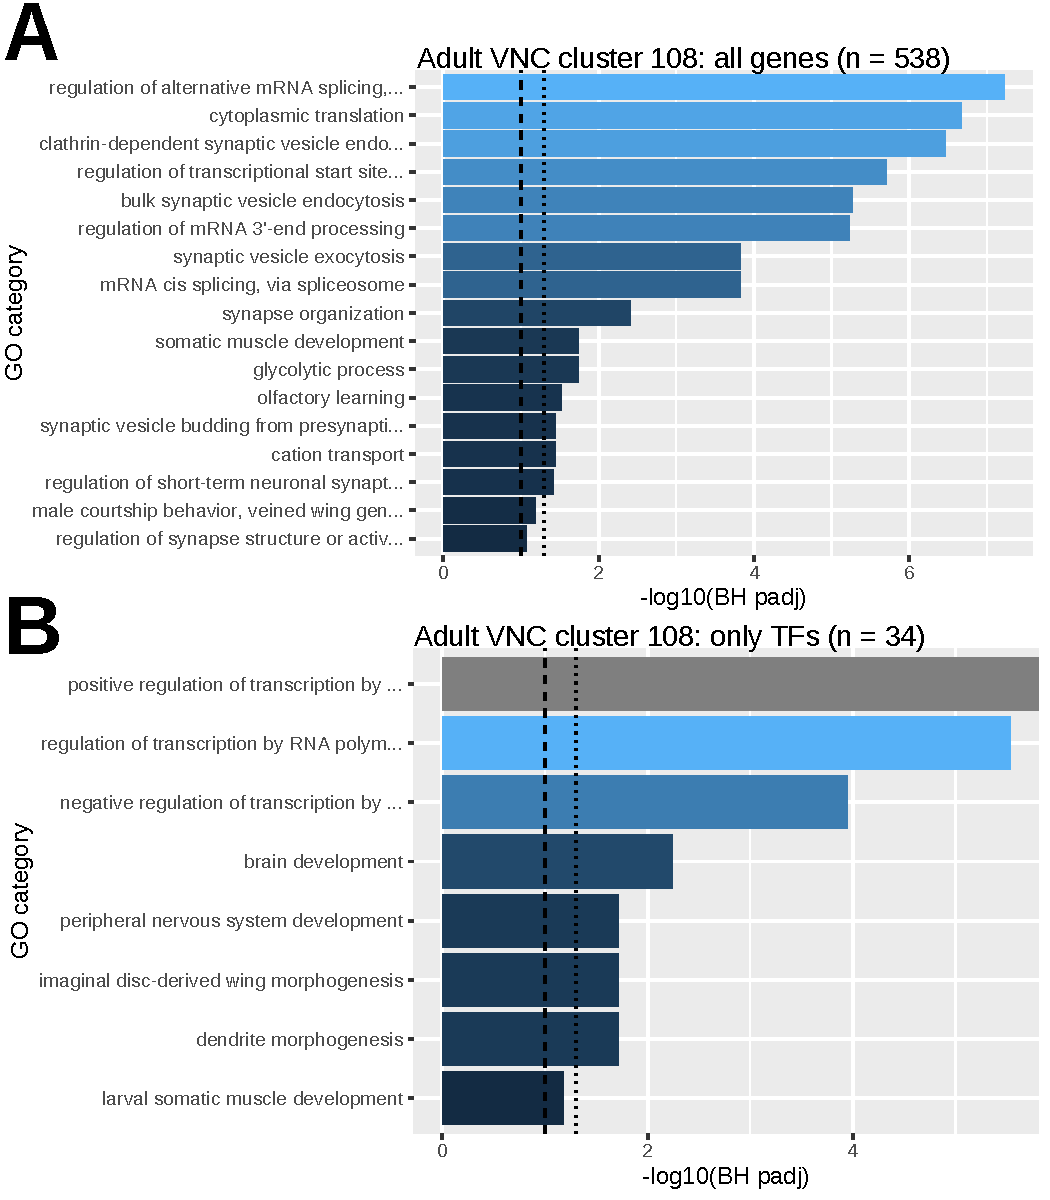
\includegraphics[width=\dimexpr.75\textwidth\relax,keepaspectratio]{figs/Fig21 allen cluster108_TFs.pdf}
\label{fig21}
\caption{\textbf{Gene Ontology enrichment for adult ventral nerve cord cluster 108.} \emph{SoxN} and \emph{D} are significant markers for cluster 108 of the adult VNC dataset. \textbf{A)} Enrichment plot of all 538 annotated genes within cluster 108. \textbf{B)} Enrichment of the 34 annotated TFs in the cluster.}
\end{figure}

\setcounter{figure}{22-1}
\begin{figure}[htbp]
\centering
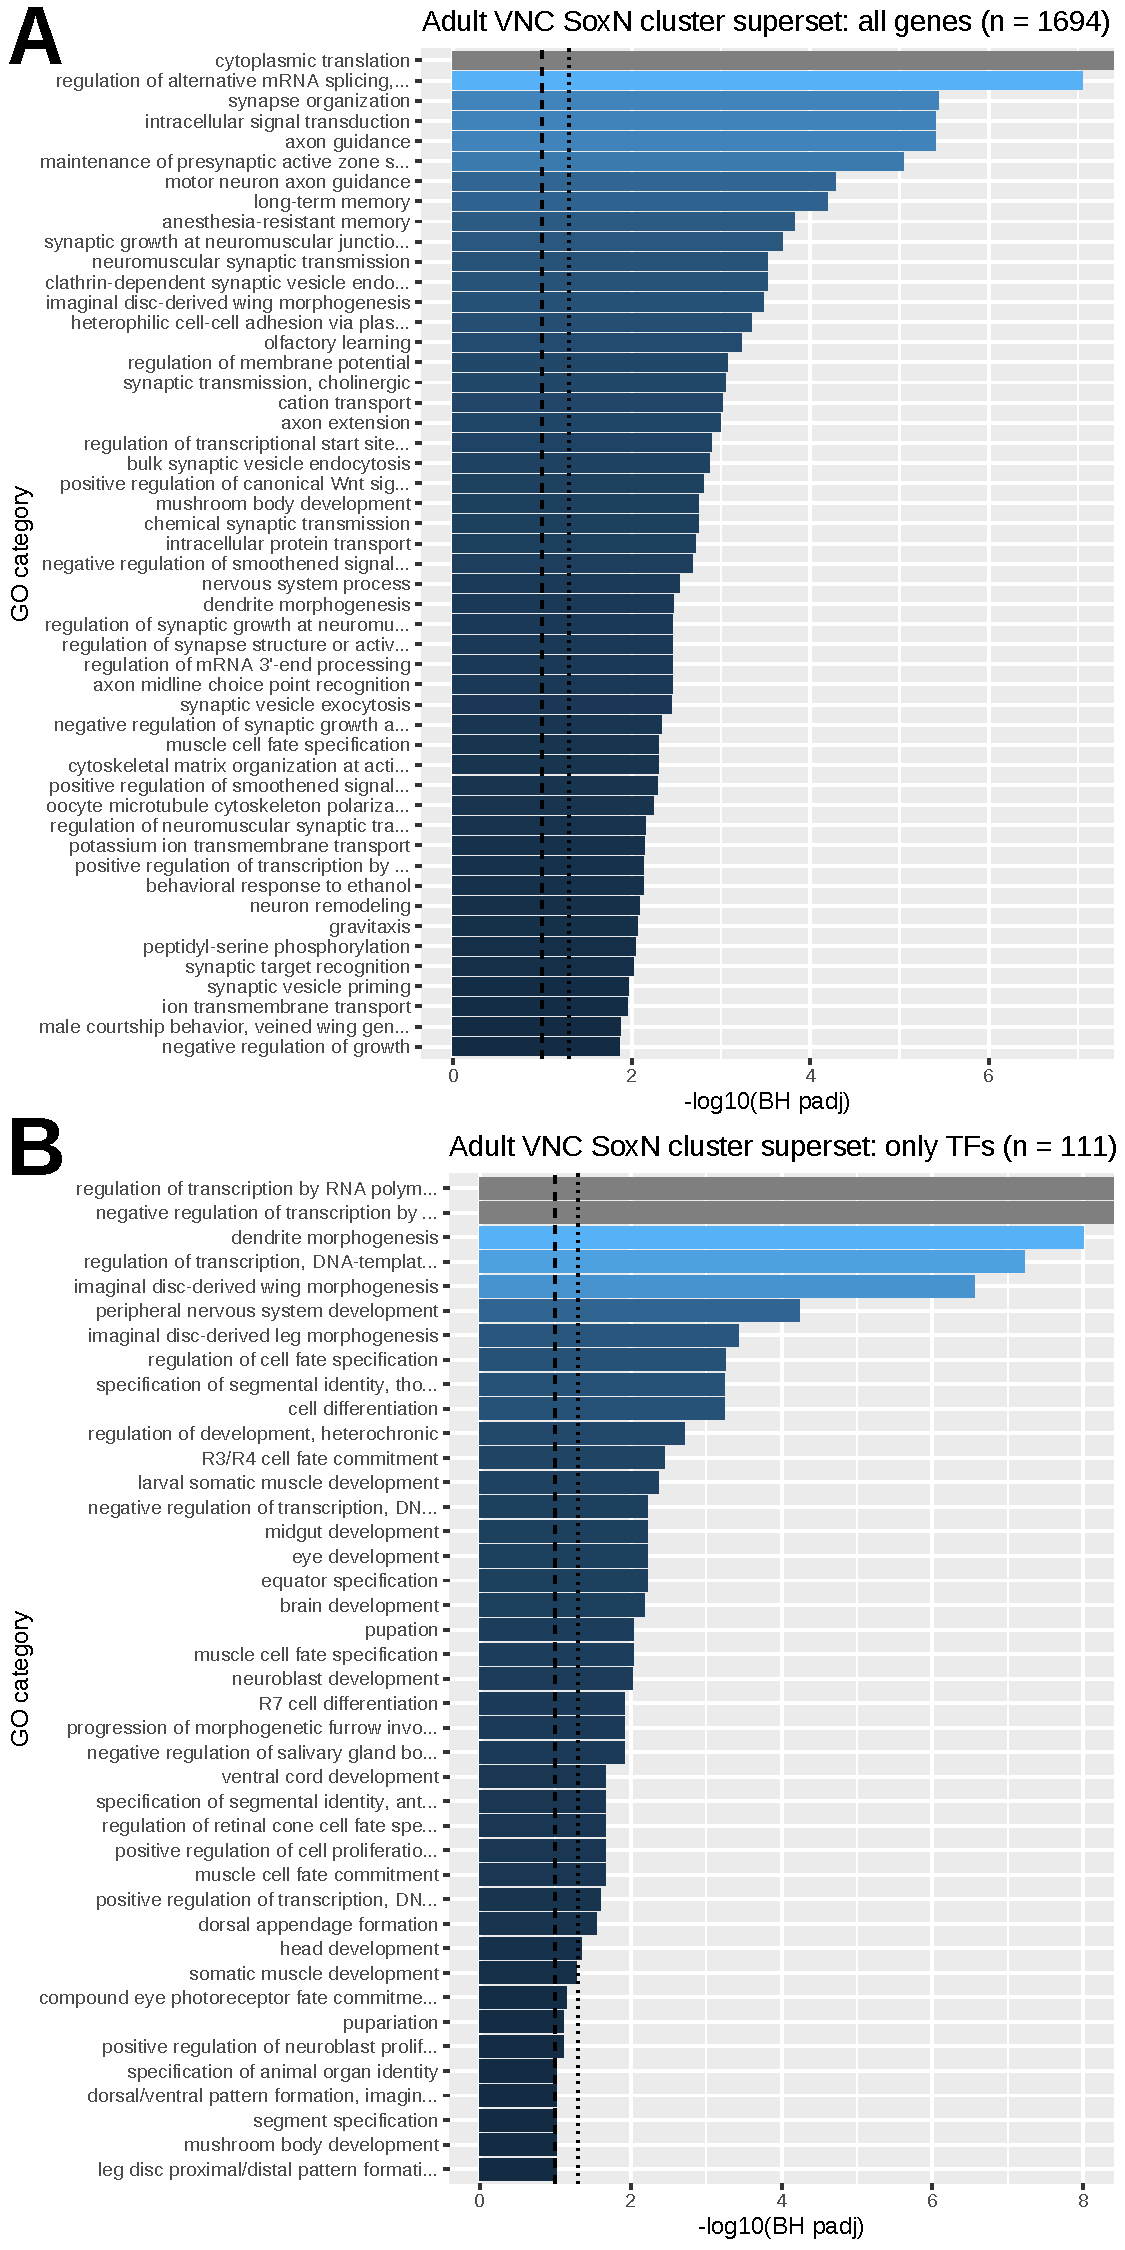
\includegraphics[height=\dimexpr\textheight-68pt\relax,keepaspectratio]{figs/Fig22 allen SoxN_clusterSuperset.pdf}
\label{fig22}
\caption{\textbf{Gene Ontology enrichment for superset of adult ventral nerve cord \emph{SoxN}-marked clusters.} This superset of a clusters that feature \emph{SoxN} as a marker includes clusters 53, 108, 126, 135, 140, 151, 159, and 167. \textbf{A)} Enrichment plot of all 1694 annotated genes within this superset. \textbf{B)} Enrichment plot of the 111 annotated TFs in the superset.}
\end{figure}

Within the superset of the \emph{SoxN}-positive clusters, the most
enriched GO terms for these 1694 genes involve translation, mRNA
splicing, signal transduction, and several functions related to the
formation of axons and synapses (Figure 22a). Focusing only on the 111
TFs within this \emph{SoxN} superset, the most significant terms include
dendrite morphogenesis, PNS development, and a variety of other specific
terms related to developmental processes (Figure 22b). Additionally,
other terms specify differentiation and development for body parts
including the brain, eyes, midgut, and muscles. Estacio-Gómez \emph{et
al.} recently described a DamID based
analysis of factors associated with particular neuronal lineages \shortcite{estacio-gomez_dynamic_2020}. They
report several TFs associated with the specification of cholinergic,
GABAergic and glutamergic neurons, including \emph{Ets65A}, a repressor
of cholinergic lineages. This TF is enriched in clusters 53, 135, and
167, indicating these are unlikely to be cholinergic (however, see
below). In contrast, \emph{knot} is reported to be a cholinergic marker
and is identified in cluster 140. Finally, \emph{Ptx1} is enriched in
GABAergic lineages and we found this only in cluster 159. Restricting
the superset to \emph{SoxN} bound targets, 414 genes are enriched for
functions mainly related to axon (\emph{p} \textless{} 3.2\textsc{e}-5) and
dendrite (\emph{p} \textless{} 3.2\textsc{e}-5) development as well as several
behavioral traits related to learning, memory, and response to ethanol.
This paints a picture of \emph{SoxN} in the adult VNC being involved in
the networks that regulate the specification and development of
particular neuronal lineage, with most of the clusters under
consideration likely to be neurons. This is in line with previous work
showing \emph{SoxN} involvement in late neuronal differentiation in the
embryo \shortcite{ferrero_soxneuro_2014}.

Turning to each cluster in turn: 53 contains 578 genes and is enriched
for synaptic transmission and organisation terms as well as olfactory
learning (Figure 23). As noted above, expression of \emph{Ets65A} would
suggest this cluster contains non-cholinergic cells; however, the
cluster contains 6 nicotinic acetylcholine receptor subunit genes which
are indicative of cholinergic functions, as well as the chloride channel
\emph{Rdl} which is associated with GABAergic activity \shortcite{mcgonigle_rdl_2009}. This may suggest the cluster contains cells of mixed
lineage. The 45 TFs in this cluster show weak enrichment
($\sim{}$3\textsc{e}-3) for processes related to eye and PNS
development, suggesting that it either comprises nerves that handle
sensory input or is simply a more general reflection of neurogenesis,
with at least 8 of the TFs known to have roles in axonogenesis.

\setcounter{figure}{23-1}
\begin{figure}[htbp]
\centering
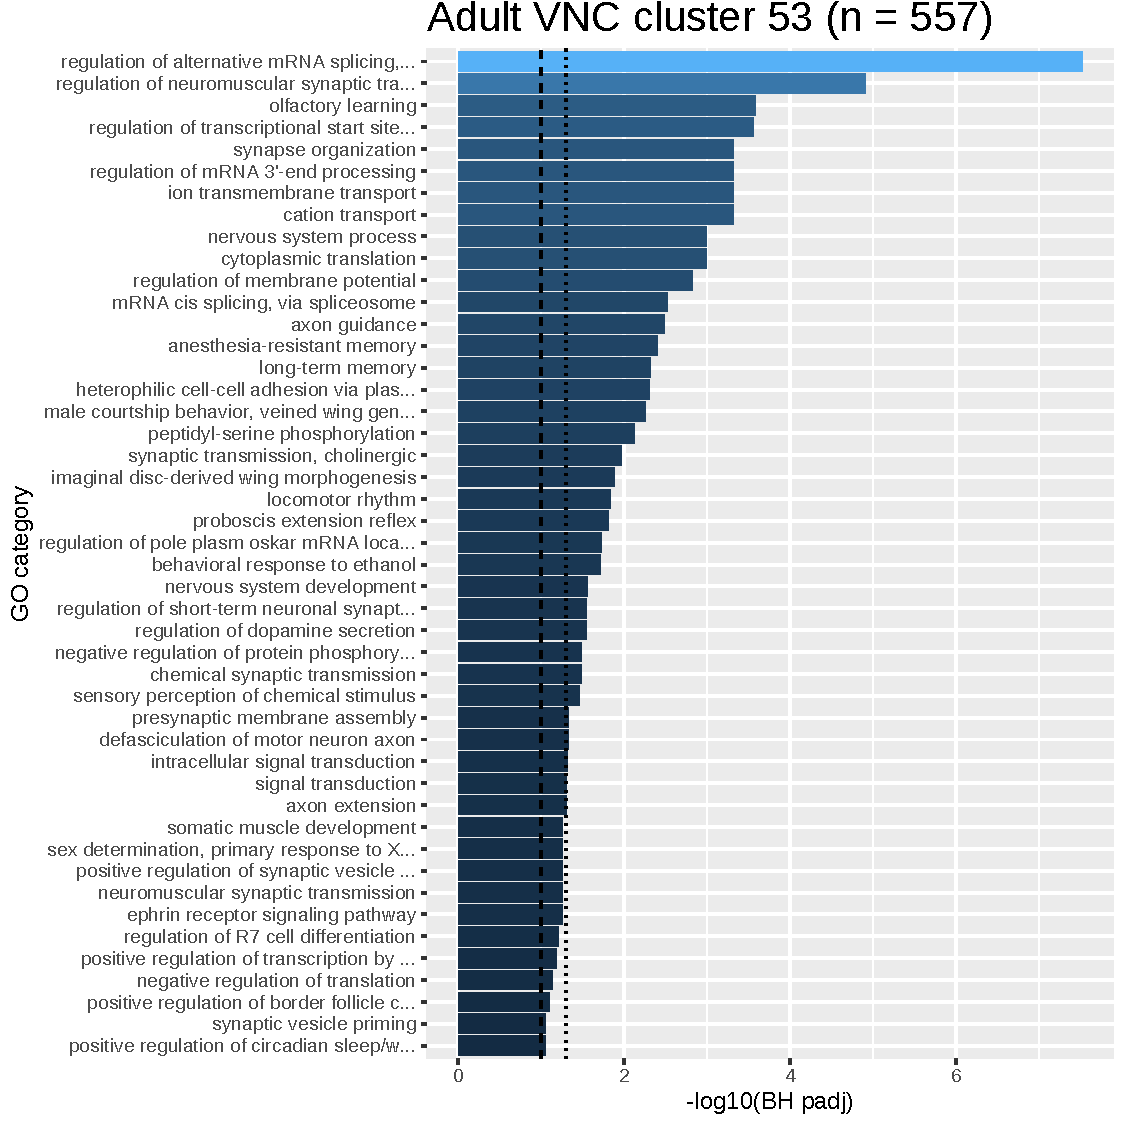
\includegraphics[width=\dimexpr\textwidth\relax,keepaspectratio]{figs/Fig23 allen cluster53.pdf}
\label{fig23}
\caption{\textbf{Gene Ontology enrichment for adult ventral nerve cord cluster 53.} \emph{SoxN} is a significant marker for cluster 53 of the adult VNC dataset. GO plot shows enrichment for the 557 annotated genes in this cluster.}
\end{figure}

\setcounter{figure}{24-1}
\begin{figure}[htbp]
\centering
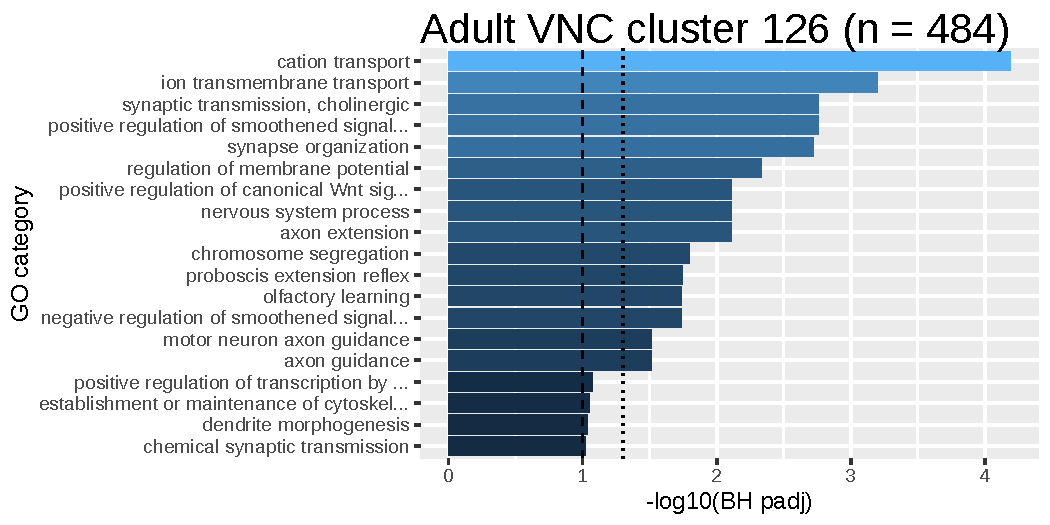
\includegraphics[width=\dimexpr\textwidth\relax,keepaspectratio]{figs/Fig24 cluster126.pdf}
\label{fig24}
\caption{\textbf{Gene Ontology enrichment for adult ventral nerve cord cluster 126.} \emph{SoxN} is a significant marker for cluster 126 of the adult VNC dataset. GO plot shows enrichment for the 484 annotated genes in this cluster.}
\end{figure}

\setcounter{figure}{25-1}
\begin{figure}[htb]
\centering
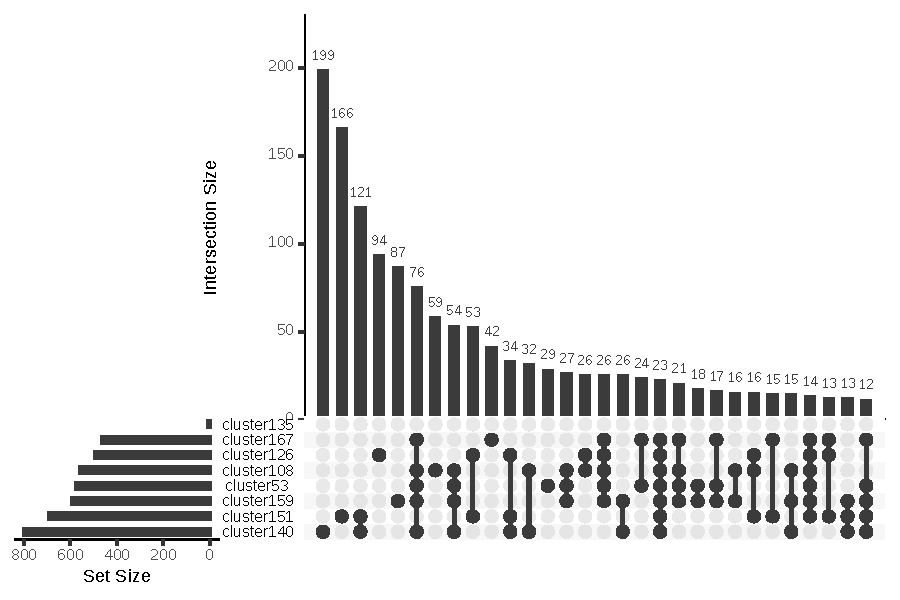
\includegraphics[width=\linewidth]{figs/Fig25 Allen upset adhoc.pdf}
\label{fig25}
\caption{\textbf{UpSet plot of adult ventral nerve cord dataset clusters.} The 30 largest intersection sets for marker genes in the \emph{SoxB}-positive clusters 53, 108, 126, 135, 140, 151, 159, and 167 are shown. Cluster 135 did not contain any marker genes that were in these largest intersection sets. Clusters 141 and 150 show a high degree of overlap in their marker genes, with a total of 121 genes uniquely shared by these two clusters.}
\end{figure}

\setcounter{figure}{26-1}
\begin{figure}[!htb]
\centering
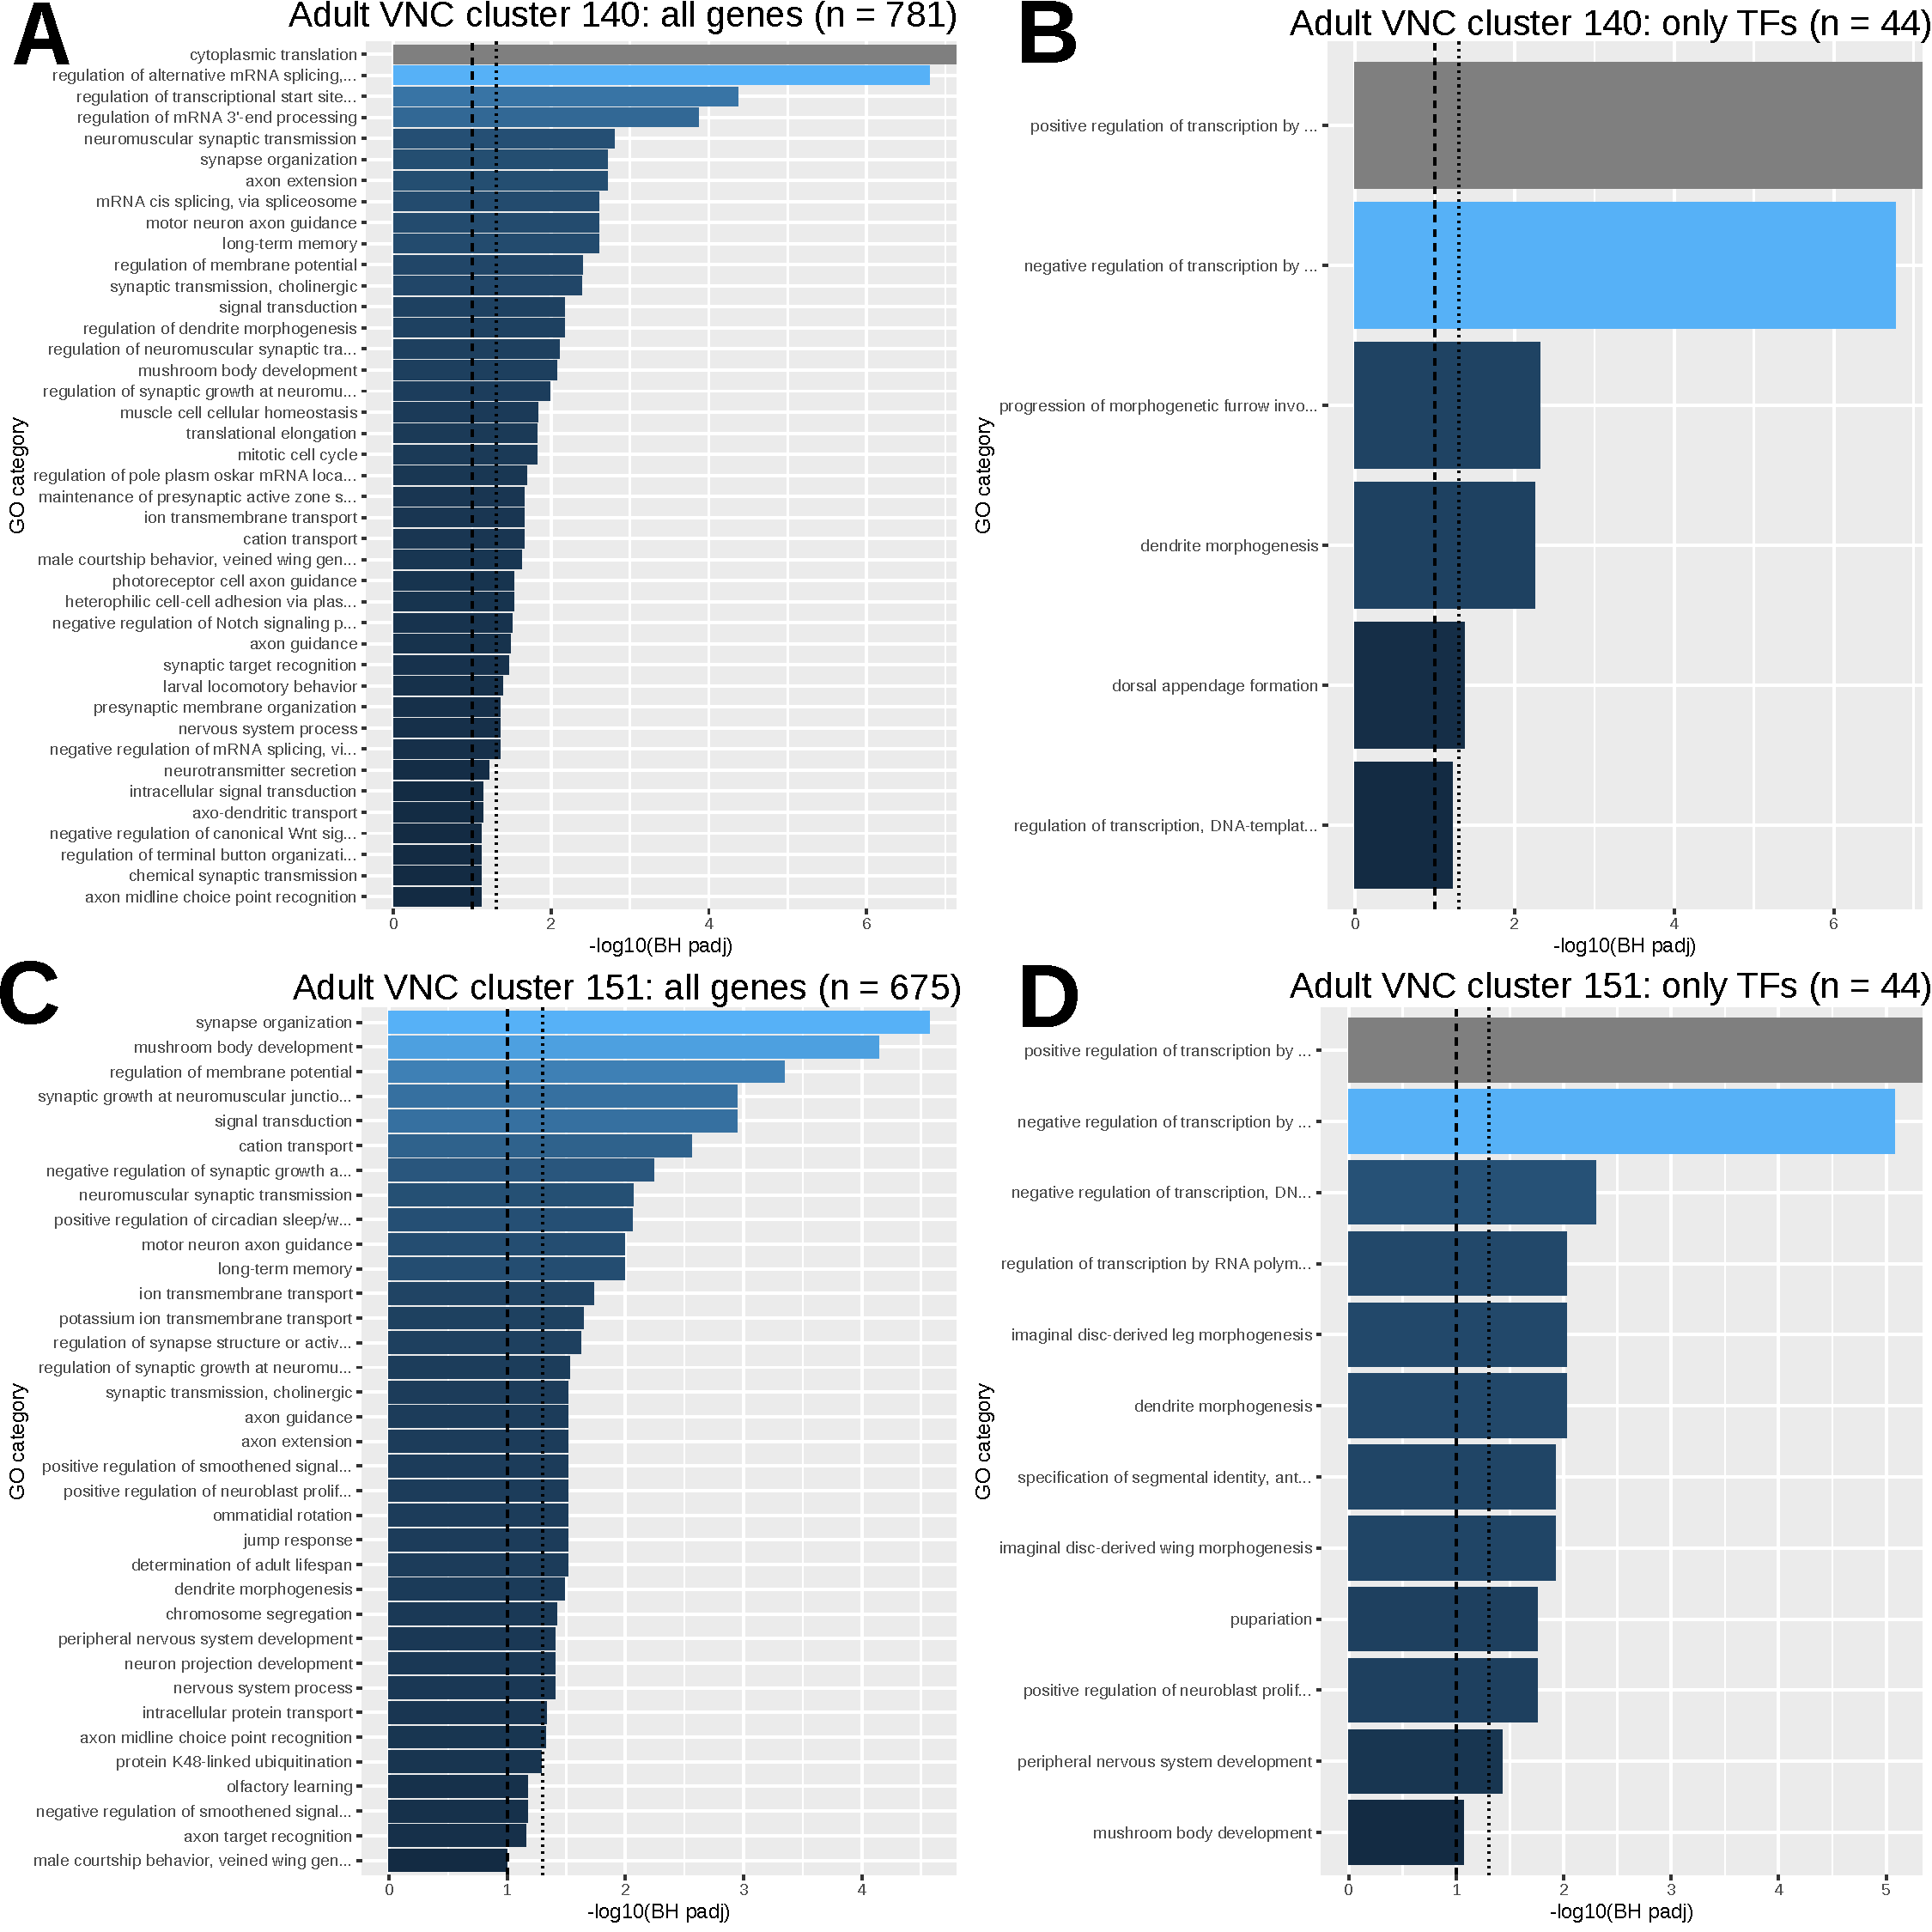
\includegraphics[width=\dimexpr\textwidth\relax,keepaspectratio]{figs/Fig 26 allen clusters 140 and 151.pdf}
\label{fig26}
\caption{\textbf{Gene Ontology enrichment for adult ventral nerve cord clusters 140 and 151.} \emph{SoxN} is a significant marker for these clusters the adult VNC dataset. \textbf{A,C)} Enrichment plot of all 781 and 675 annotated genes in clusters 140 and 151, respectively. \textbf{B,D)} Enrichment of the 44 annotated TFs in each cluster.}
\end{figure}

\setcounter{figure}{27-1}
\begin{figure}[!htbp]
\centering
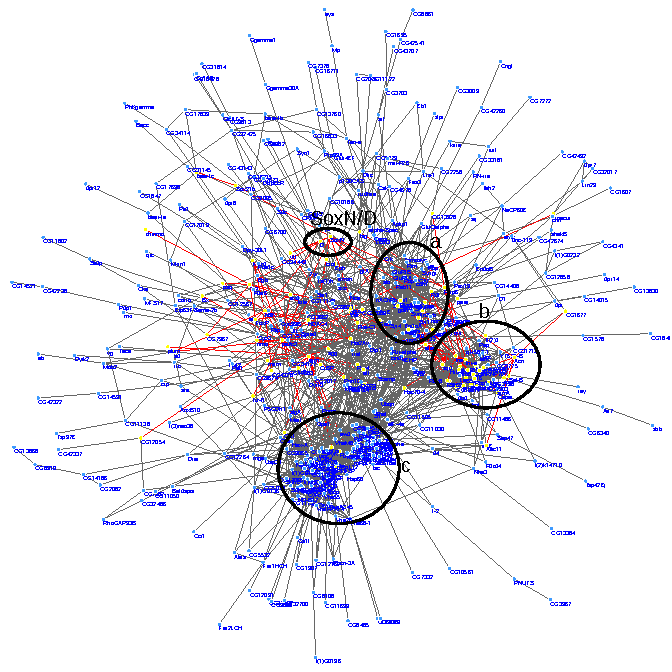
\includegraphics[width=\textwidth]{figs/Fig27 Network v2}
\label{fig27}
\caption{\textbf{Gene Regulatory Network for adult ventral nerve cord cluster 108.} Visualised in Cytoscape, this GRN uses an edge-weighted spring embedded layout to yield an undirected graph of interactions in the sole cluster expressing both \emph{SoxN} and \emph{D} as marker genes. Line weights are proportional to STRING database experimental evidence annotations for protein-protein interaction. Nodes within two degrees of separation from \emph{SoxN} and \emph{D} are highlighted in yellow and are connected by red lines. Three main clusters of genes deal with functions related to synapse neurotransmission, transcriptional regulation, and metabolic maintenance, respectively. Genes within two degrees of \emph{SoxN} and \emph{D} appear to provide regulatory entry points into these clusters, as well as to other genes not part of these clusters.}
\end{figure}

Cluster 126 contains 484 genes that are highly enriched for ion
transport and cholinergic synaptic transmission, as well as more general
terms related to axon/synapse development (Figure 24). As with cluster
53, it contains several nAChR subunit genes, suggesting that these cells
are likely cholinergic. Enrichment for Wnt and Hh (via Smo) signalling
is associated with neural development and processes such as planar
polarity \shortcite{mcfarland_hh_2008} as well as axon guidance \shortcite{charron_hedgehog_2007}, and may indicate that these cells are
differentiating. This cluster is also enriched for the functional terms
proboscis extension and olfactory learning, perhaps suggesting that they
are differentiating progenitors that have initiated specific neural
expression programmes.

Cluster 135 only contains 9 genes, 4 of which encode mitochondrial
proteins related to electron transport and ATP production. It contains
\emph{SoxN} and the cholinergic repressor \emph{Ets65A}. It is possible
that this small cluster is simply an artifact of the partitioning
approach.

Clusters 140 and 151 are the most similar of any two clusters, with 121
genes in common that are not shared by any of the other SoxB clusters
(Figure 25); both are enriched for synapse formation and development,
suggesting their GRNs play a role in organising the growing CNS, and in
the case of cluster 151, also the PNS (Figure 26a,c). It is worth noting
that cluster 140 contains the \emph{knot} TF, a marker for cholinergic
neurons, along with the fly Acetylcholine esterase and Choline
acetyltransferase genes (\emph{Ace} and \emph{ChAT}), reinforcing the
view that these are cholinergic neurons. In contrast, cluster 151
expresses Tropomyosin 1 (\emph{Tm1}), a gene enriched in L3 larval
GABAergic neurons \shortcite{estacio-gomez_dynamic_2020}. While the 44 TFs within
cluster 140 show relatively few significant ontology enrichments, the 44
TFs in cluster 151 are enriched for regulators implicated in PNS
development (Figure 26b,d), perhaps suggesting that, given their
similarity, 151 cells are progenitors of cluster 140 neurons.

Though cluster 159 appears similar to other clusters, with enrichment
for genes involved with synaptic formation and organisation, it also
appears to contain TFs involved with morphogenesis and PNS formation,
with weak enrichment for TFs implicated in the regulation of cell
proliferation. The cluster contains the \emph{Ptx1} TF and other markers
found in GABAergic neurons, but also features two nAChR subunits and the
muscarinic Acetylcholine receptor (\emph{mAChR-A}), which are more
associated with cholinergic neurons. The presence of mixed
neurotransmitter types and positive regulators of cell proliferation
shuch as \emph{Tsh} and \emph{Hth}, may suggest this cluster represents
progenitors.

Cluster 167 genes appear enriched for mRNA regulation and ion transport,
with a number of ontology terms pointing to aspects of neuronal
differentiation (synaptic functions, axon differentiation/guidance)
while its TFs show some enrichment for eye development terms indicative
of general neuronal functions.

\subsubsection{\emph{SoxN} and \emph{D} Compensation}

In cluster 108, both \emph{SoxN} and \emph{D} are expressed, signifying
that genes in this cluster may provide insight to the shared parts of
the GRN that allow one factor to partially compensate in the absence of
the other. Using Cytoscape with the edge-weighted spring embedded
layout, it was possible to visualise the GRN of cluster 108, as well as
the degrees of separation between \emph{SoxN}/\emph{D} and the rest of
the network (Figure 27). Within two degrees of separation, there are 92
other genes in the vicinity of the two SoxB factors, and several of
these genes appear closely linked to dense clusters within the network.
Cluster A appears on the top of the network and contains 47 genes whose
GO terms are highly enriched for synapse formation, neurotransmission,
and sensation. Cluster B is on the right of the network and contains
nodes close to cluster A; its 35 genes are enriched for functions
related to the regulation of mRNA slicing and processing. Cluster C on
the bottom of the GRN is the furthest separated from the other clusters
and contains a dense network of 73 genes related to translation as well
as metabolic processes such as electron transport and ATP production.



Each of these three clusters represents a different subset of genes that
\emph{SoxN} and \emph{D} may be able to regulate through various
pathways. Supplementary Table 1 provides a full list of genes in each
cluster, as well as the genes in the regulatory vicinity of the Sox
genes. Within clusters A-C, 24.7\% and 34.7\% of the 170 genes are bound
by SoxN or D in the embryo respectively, in line with the average of
23.3\% and 39.8\% for the 558 genes throughout cluster 108. This rises
to 35.5\% and 60.1\% (\emph{z} $=$ 2.511 and 4.684, two population Z test)
when considering the genes in the vicinity of \emph{SoxN} and \emph{D}
within the network.

Examining these genes within two degrees of separation of \emph{SoxN}
and \emph{D}, the most enriched terms involve transcriptional
regulation, mRNA processing, and processes related to cellular
signalling and stem cell maintenance. These genes include \emph{Sox21b}
as well as neural markers like \emph{pros} and \emph{elav}.
Additionally, this group contains 15 of the 34 TFs in the entire cluster
108. Interestingly, several of the genes within two degrees of the Sox
genes provide entry points to the other regulatory clusters. Clusters A
and B appear to contain several genes that interact with the
differentiated neuron marker \emph{elav} \shortcite{yankura_gene_2013}, while
cluster C metabolic genes \emph{Tpi} and \emph{Pgk} are linked to the
beta-catenin homologue \emph{arm} that is involved in Wnt signalling and
segment polarity \shortcite{loureiro_roles_1998}. A central group of the
genes \emph{pros}, \emph{dnc}, and \emph{Lar} extends its connections to
other genes in the network that are not parts of the main three
clusters. While these connections require empirical testing for further
confirmation, the parts of this GRN within two degrees of separation
from \emph{SoxN} and \emph{D} represent potential regulatory entry
points for Sox genes to regulate transcription, metabolism, and
neurotransmission within differentiated nerve cells. Overlaps in these
networks may reveal the shared targets that allow either gene to
partially compensate for the other.

The analysis of this large single cell dataset uncovered some
interesting insights but also some confusing observations. While in
general \emph{SoxN} is associated with the expression of TFs implicated
in aspects of neuron development and differentiation, the clustering
approach combined cells expressing markers indicative of different
neuronal functions (cholinergic and GABAergic). The consistent
enrichment for genes associated with neuronal activity, such as axons,
synapse functions and, in particular, neurotransmitters, strongly
suggests these are not neuroblast lineages. Thus the analysis either
indicates that \emph{SoxN} is expressed in progenitors that give rise to
neurons of different fate, or the clustering method is combining cells
of different lineage. Nevertheless, the analysis has uncovered sets of
genes expressed in particular cell types that are likely to be direct
SoxB targets in the adult CNS.

\subsection{Comparing Datasets}

After assigning cell identities to clusters in each dataset, it was of
interest to explore whether any of these clusters could correspond to
others at different developmental stages. Using the ClusterMap software,
the embryo and larval brain as well as the larval brain and adult VNC
datasets were compared. While the software was able to identify
correlations between clusters, none of these correlations were
significant enough to conclude a relation between any two datasets.
Within the embryonic-larval comparison, the \emph{SoxN}-positive larval
clusters 6, 7, 8, and 10 exhibited a similarity score of only 0.04 to
embryonic cluster 10; for the larval-adult VNC comparison, they did not
map onto any of the VNC clusters. It was not possible to perform this
automated correlation between datasets, so drawing conclusions from the
data required exploring the literature to infer how clusters from one
dataset could relate to another.

\subsection{Data Reliability}

While the methods used for this analysis aimed to provide a consistent process for evaluating multiple datasets systematically, the drawback of this approach is that it produces results that differ from the originally published analyses for these datasets. The lack of data filtering and normalisation was intended to avoid discarding signals that are potentially biologically relevant. Indeed, as expression of \emph{D} was more restricted than that of \emph{SoxN}, this approach helped ensure that even lowly-expressed genes could be captured by this analysis. 

However, there are potential pitfalls of this approach. Lack of filtering has the potential to decrease the signal-to-noise ratio within the data, and instead favors false positives over false negatives. This leaves the analysis susceptible to artifacts of bias from the sequencing methodology, which is amplified by the fact that scRNA-seq data is inherently more noisy than bulk RNA-seq data \shortcite{chen_single-cell_2019}. Particularly, while the 10X Chromium method used for the adult VNC dataset allows for cheap profiling of a high number of cells compared to methods like Smart-Seq2, the number of detected genes per cell is considerably lower \shortcite{baran-gale_experimental_2018}. While the log transformation used in this analysis accounts for some of the variability in low-count genes, other normalisation methods like the sctransform variance-stabilised transformation make fewer assumptions about the underlying structure of the data \shortcite{hafemeister_normalization_2019}. Given the potentially biased structure of the data and the goal of identifying as many leads as possible, the subjective determination of this analysis was to decrease false negatives even at the expense of increasing false positives. Therefore, the lack of filtering and normalisation beyond the standard log-transformation had the possibility to incorporate artifacts of bias into the results relative to the original analysis by Allen \emph{et al}.

Another factor to consider is that the UMAP method used to categorise clusters of cells is based on a stochastic process and is therefore less reproducible than deterministic dimensionality reduction algorithms like PCA. The consequence of this is that performing the same UMAP reduction with different seed values has the potential to a produce a different clustering of cells each time. For this analysis, the default seed value of 1 was used each time for consistency. However, because of the bias added by omitting the filtration and extra normalisation steps, it was necessary to ensure that the clusters produced by these analyses had some biological validity based on correlation to the clusters determined by Allen \emph{et al}.

Marker gene lists for \emph{SoxN}-positive and \emph{D}-positive clusters were obtained from the SCope database \shortcite{davie_single-cell_2018} and compared to the corresponding clusters from this unfiltered analysis. Allen \emph{et al}. identified 10 \emph{SoxN}-positive clusters, 2 \emph{D}-positive clusters, and one cluster positive for both. The marker gene lists for the superset of the \emph{SoxN} clusters was compared to the corresponding list for the \emph{SoxN} clusters in the unfiltered analysis; likewise, the process was repeated for the \emph{D} clusters and for the clusters expressing both.

The Jaccard similarity of the corresponding gene lists from each analysis were relatively low (0.128 comparing \emph{SoxN} clusters, 0.065 comparing \emph{D} clusters, and 0.037 comparing \emph{SoxN-D} clusters), suggesting that the gene lists that these analyses produced were highly dissimilar. However, upon closer inspection, these low values are explained by the fact that the gene lists in the unfiltered analysis were significantly more expansive than those identified by Allen \emph{et al.}; this is expected, as the goal of the unfiltered analysis was to be unrestrictive in order to reveal more candidate genes. When considering the percentage of genes identified by Allen \emph{et al}. that were also detected in this analysis, there is considerably more overlap. For the \emph{SoxN}-positive clusters, 78.8\% of marker genes overlapped with the gene lists produced in the unfiltered analysis. For \emph{D} clusters and \emph{SoxN-D} clusters, these values were similarly high at 80.4\% and 80.8\%, respectively. This signifies that while the two methods produced different cell clusters, the clusters that were identified as positive for either gene were robust between analyses, lending validity to the idea that this consistent unfiltered approach produces results that are biologically similar to the original filtered analyses while also identifying more candidate genes.

Because these methods produced different results, the intersection sets of their gene lists are of particular interest because they represent the most high-confidence marker genes for \emph{SoxN} and \emph{D} clusters. The consensus marker list for \emph{SoxN}-positive clusters includes 231 genes enriched for nervous system development (\emph{p} $=$ 1.65\textsc{e}-13) and neuron differentiation (\emph{p} $=$ 2.08\textsc{e}-13), consistent with known roles of \emph{SoxN} in later neuron differentiation. The 31 genes in the \emph{D} consensus list were enriched for localisation in the embryonic brain (\emph{p} $=$ 1.59\textsc{e}-6) and ventral midline (8.94\textsc{e}-6), consistent with known roles of \emph{D} regulating earlier brain development and later localisation in the midline \shortcite{aleksic_role_2013}. The 21 consensus genes from the \emph{SoxN-D} clusters exhibit low expression during early embryogenesis (1 gene) with increasing expression until peak expression at stages 13-16 (12 genes), consistent with the idea that \emph{SoxN} and \emph{D} pathways are considerably active after stage 11 of embryonic development \shortcite{ferrero_soxneuro_2014}.

While these consensus sets give insight into the most reproducible marker genes, it is also of interest to characterise the $\sim{}20$\% of genes in each category identified by Allen \emph{et al}. which were not identified by the unfiltered analysis. For all three categories of gene lists, there were too few genes to yield significant GO enrichment when compared to a background gene set of all \emph{Drosophila} genes. The GO analysis was repeated to consider the background set as only the genes in the union of the gene lists from the two analyses, with similar inconclusive results. However, when looking only at the enrichment for the consensus set of \emph{SoxN}-positive clusters, there was a significant enrichment for motor neuron axon guidance (\emph{p} \textless{} 10\textsc{e}-2). None of the other intersection sets exhibited significant enrichments when compared to their corresponding restricted background gene sets. Taken together, though, these results show that the gene lists produced by the unfiltered analysis produced largely similar cell type clustering and marker gene lists as compared to the original analysis. This lack of difference suggests that the algorithmic deviations still preserved significant consensus genes while also allowing for more genes to be considered in each gene set.

\section{Discussion}

These computational experiments represent a more nuanced understanding
of the expression of \emph{SoxN} and \emph{D} \emph{in vivo} based on a
systematic scRNA-seq approach. Most of the Sox-positive clusters in the
embryo and larval brain appear to be NPCs and maturing neuroblasts/GMCs,
while in the adult VNC, Sox genes are expressed in differentiated
neurons. Examining the marker genes in each cluster provided an idea of
the factors that are regularly coexpressed with \emph{SoxN} and
\emph{D}, and through GO analysis it was possible to examine the
different cellular functions carried out in each tissue. Annotations for
TF status as well as \emph{SoxN} and \emph{D} binding gave a focused
view at the factors that most likely work with Sox genes directly to
influence the expression of other structural genes in each cluster.

While this approach approximates a systematic and unbiased approach,
there are definite pitfalls of the methods used. Within the embryonic
dataset, for instance, cluster 5 showed \emph{D} as a marker gene, but
after Benjamini-Hochberg correction, it was no longer a significant
marker for that cluster. The aim of this project was to be permissive in
identifying potential candidates in the Sox interactome, and therefore,
\emph{D} was still considered as a marker for this cluster despite low
significance. Additionally, identifying marker genes within each cluster
uses the Wilcoxon rank sum test, a nonparametric measure that tests
whether the prevalence and intensity of a given gene's expression level
is higher within a cluster as compared to cells outside the cluster.
Because of how significance is calculated, it is often the case that
certain genes will not be counted as markers if they are ubiquitous and
not uniquely expressed. Despite the fact that the larval brain dataset
exhibited some \emph{D} expression in multiple clusters (Figure 12c),
\emph{D} was not a significant marker gene for any cluster. However, as
stated before, several of the gene targets within clusters 6, 7, and 8
are \emph{D} binding targets in the embryo, and even a baseline level of
presence may be possible for \emph{D} to regulate expression in those
cells. For this reason, the list of genes in each marker list is a
suggestive but non-exhaustive look at the unique expression within
different cell groups.

Many of the cell type inferences depended upon performing Gene Ontology
enrichment analyses for each set of genes. This was a useful first-pass
filter for understanding the main biological processes occurring in each
cell cluster. However, GO analysis is a flawed metric notorious for
yielding false positives \shortcite{pavlidis_critical_2012}, so any GO enrichment
scores must be viewed with caution. Because of how enrichment is
calculated, the validity of results can vary depending on the number of
genes being examined and the degree to which they are annotated with GO
functions. Ostensibly, future analysis with more complete gene
annotations may result in different GO terms appearing as enriched. For
this reason, the GO analysis was used primarily as a guide rather than
as a standard. By examining common GO terms within each cluster or group
of clusters, it was possible to see how GO terms changed when focusing
on subsets such as TFs and bound genes; after that, manual examination
of each list was necessary for drawing meaningful conclusions from the
data. Future analyses may seek to provide a finer resolution of inference by restricting the background gene sets---for instance, when evaluating only the TFs within a larger gene list, it may be beneficial to use the list of annotated TFs as a background set rather than the full \emph{Drosophila} genome so that significant terms are less heavily biased towards GO terms involving transcriptional regulation.

The attempted unbiased approach for processing each dataset allowed the
same pipeline to apply to multiple unrelated sequencing projects. While
this provided consistency between datasets, this came at the expense of
congruity with the original results. In the larval brain dataset,
clusters 6, 7, 8, and 10 appear to be related to one single cluster from
the original analysis by Avalos \emph{et al}.; however, because the
cluster grouping in this analysis was different, it was possible to see
how cluster 10 may be a more mature version of the cells in the other
clusters. However, it is still possible that some of the incongruity may
also be because the lack of low-count filtering in this analysis
introduced statistical noise that biased the data. Despite this, comparison of clusters in the unfiltered adult VNC analysis against clusters produced originally by Allen \emph{et al}. indicate a relatively high degree ($\sim{}$80\%) of replicability along with sufficient permissiveness to identify more candidate genes than the original analysis. This indicates that despite deviations from the original analyses caused by lack of filtration or normalisation, and despite the stochastic nature of the UMAP algorithm, the identified clusters were still robust and can meaningfully be used to draw inference about the underlying regulatory biology. This reflects the fact that UMAP tends to favor high reproducibility and biological validity when compared to other nondeterministic algorithms like t-SNE and scvis \shortcite{becht_dimensionality_2018}. The unfiltered approach contained the added benefit of systematic consistency of analysis among different datasets, and largely preserved gene list structure while also identifying more potential hits.

While comparisons between datasets attempted to hold all factors
constant, this was not always possible. For instance, the adult VNC
dataset was an order of magnitude larger than the others, and was run on
the Rustbucket server because analysis was not possible on a local
machine. However, for the sake of computational efficiency, only male
flies were pooled for the final dataset. This decision was arbitrary and
can be trivially modified to include female flies instead; however, the
failure to include female samples in this analysis can be seen as an
example of sex bias in scientific research \shortcite{lee_sex_2018}. With
access to higher computing power, it would be possible to repeat the
analysis with two male and two female replicates in order to lend higher
validity to these findings. However, the approaches used to study the
GRNs in these male flies is versatile and can be applied to a network
that includes both males and females.

Overall, these computational experiments detail a process for extracting
information about Sox genes from preexisting public datasets. Using GO
analysis to identify significant processes, subset analysis to highlight
genes of interest, and network analysis to uncover the structure of shared regulatory networks, it was possible to identify putative cell 
identities as well as candidate genes for further exploration within
Sox-related GRNs. In the future, it would be worthwhile to extend this
analysis to other scRNA-seq datasets that may include more \emph{D}
expression. Because \emph{Dichaete} plays a conserved role in embryonic
patterning, it may be worthwhile to isolate \emph{D}-positive cells with
flow cytometry and then identify features of its interactome that may be
shared between species. Additionally, wet lab experiments will be
necessary to validate each of the putative leads identified in this
analysis. Methods such as co-IP and pulldown assays will be necessary to
validate whether each Sox factor physically interacts with these
identified targets. Additionally, once the
\emph{SoxN\textsuperscript{mSox2}} and \emph{D\textsuperscript{mSox2}}
constructs are ready, it will be of interest to explore whether
exogenous \emph{mSox2} interacts with target genes in the same way due
to either structural similarities or regulatory forces. These data have
identified roles in which \emph{SoxN} and \emph{D} contribute to the
function and regulation of cells throughout the development of the fly
CNS.

\chapter{Conclusion}

Sox genes play a vital role in regulating developmental processes in
flies and in animals. Understanding the SoxB genes \emph{SoxN} and
\emph{D} is a valuable step in characterising the impact that homologous
Sox genes may have in mice and in humans. This project represents an
attempt to characterise the known functional redundancies between SoxB
genes and to explore what makes them different.

Much of the wet lab portion of this thesis relies on future
experimentation to validate or reject any proposed hypotheses about how
\emph{SoxN} and \emph{D} can functionally compensated by an exogenous
homologue. The procedures detailed in the wet lab portion of this thesis
will provide sufficient detail for future experimenters to assemble the
donor templates and then use CRISPR/Cas9 to produce knock-in flies.
Whether \emph{mSox2} is indeed capable of functionally compensating for
fly Sox genes will depend on whether any phenotype is observable in the
resulting progeny. This may be in the form of macroscopic developmental
defects, CNS hypoplasia identifiable via BP102 antibody staining, or
even molecular differences in binding targets. Assuming that the
knock-in flies are viable, comparing the differences between
\emph{SoxN\textsuperscript{mSox2}} and \emph{D\textsuperscript{mSox2}}
phenotypes will provide insight to how the regulatory features of the
\emph{SoxN} and \emph{D} loci affect their expression and behavior in
the cell. If successful, this will elucidate some of the mechanisms that
allow the two genes to functionally compensate for each other, as well
as the unique structural and regulatory factors that cause them to have
different roles in development.

The computational experiments in this project represent an attempt to
leverage existing data to find new insights. The known evolutionary
history of Sox genes points to the idea that functional redundancy is
supported by conservation in gene targets and GRNs. By systematically
examining all genes at different developmental stages, it was possible
to explore the expression of \emph{SoxN} and \emph{D} \emph{in vivo} and
infer not only functions specific to each cell type but also the other
elements with which Sox genes share their GRNs. From this data, it was
possible to identify putative neuroblast and NPC cell groups at the
onset of embryonic gastrulation and in early larval development.
Additionally, expression of \emph{SoxN} in the adult ventral nerve cord
reveals groups of Sox-expressing nerve cells that specialise in
different functions. Examination of the other genes that are coexpressed
in these clusters has provided insight to possible regulatory networks
that impact shared \emph{SoxN} and \emph{D} functions, and also
demonstrate how these factors are able to impact a variety of cellular
functions in different tissues.

While these clusters have been given putative identities, there is still
more that can be learned from them. This project has looked at the
markers in cells that are positive for \emph{SoxN} and \emph{D}. This
has identified other players in these GRNs that may merit further
exploration in the lab. If any of these leads are successful, the next
step would be to use a similar process to explore regulatory networks in
the clusters positive for those validated leads. This, in turn,
represents an iterative methodology for identifying potential hits and
then exploring their expression further. Potentially, it would be of
interest to incorporate even more datasets that include greater spatial
and temporal specificity so that it may be possible to examine Sox genes
without being influenced by background expression from cells that do not
express these factors.

Sox genes are important in development throughout the animal kingdom,
and SoxB genes in particular play a vital role in segmentation and
neurodevelopment. The experiments and analyses conducted as part of this
thesis project provide a starting point for future investigators to look
at Sox expression and regulatory networks. Discoveries regarding
\emph{SoxN} and \emph{D} expression may immediately translate to a
better understanding of arthropod developmental regulation, but homology
to mammalian group B Sox genes paves a way for these insights to
potentially impact our understanding of human stem cell maintenance and
neurodevelopment.

%%%%%%%%%%%%%%%%%%%%%%%%%%%%%%%%%%%%%%%%%%%%%%%%%%%%%%%%%%%%%%%%%%%%%%%%%%%%%%%%
%% Bibliography:
%%
\cleardoublepage
\phantomsection
%\addcontentsline{toc}{chapter}{Bibliography}
\bibliographystyle{apacite}
\bibliography{thesis-minimal}



%%%%%%%%%%%%%%%%%%%%%%%%%%%%%%%%%%%%%%%%%%%%%%%%%%%%%%%%%%%%%%%%%%%%%%%%%%%%%%%%
%% Appendix:
%%

\appendix{}

\chapter{Supplementary Figures and Tables}

% Reset figure counter for supplement
\makeatletter 
\renewcommand{\thefigure}{S\@arabic\c@figure}
\makeatother
\setcounter{figure}{0}

\begin{figure}[htbp]
\centering
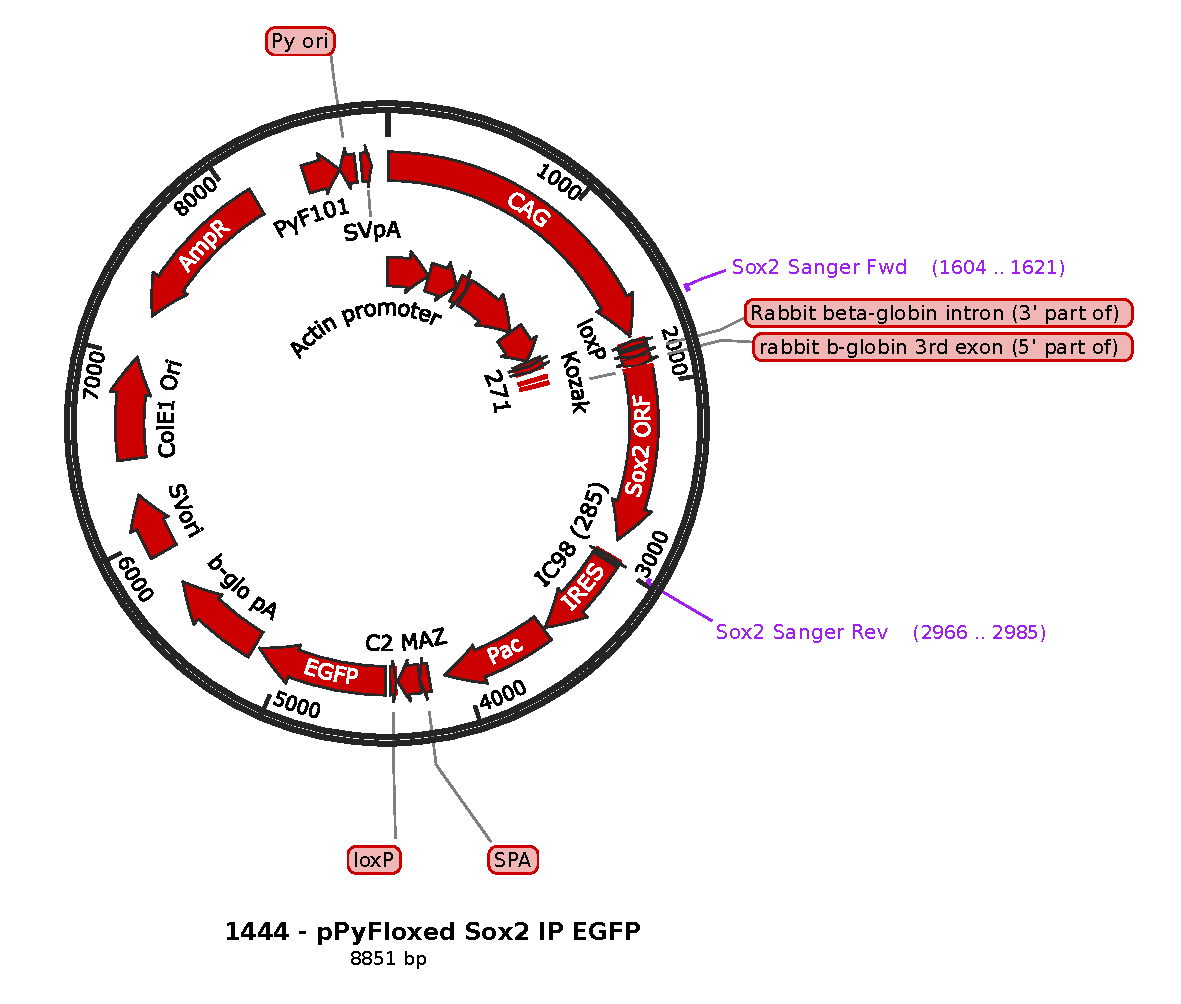
\includegraphics[width=0.9\textwidth]{FigS1_1444 - pPyFloxed Sox2 IP EGFP Map.pdf}
\label{figS1}
\caption{\textbf{Schematic of plasmid 1444 containing the mSox2 CDS.} Custom primers for Sanger sequencing are indicated, as are selection markers and other features native to the plasmid. Plasmid and annotations provided by the lab of Prof. Jennifer Nichols (Cambridge Stem Cell Institute).}
\end{figure}


\begin{figure}[htbp]
\centering
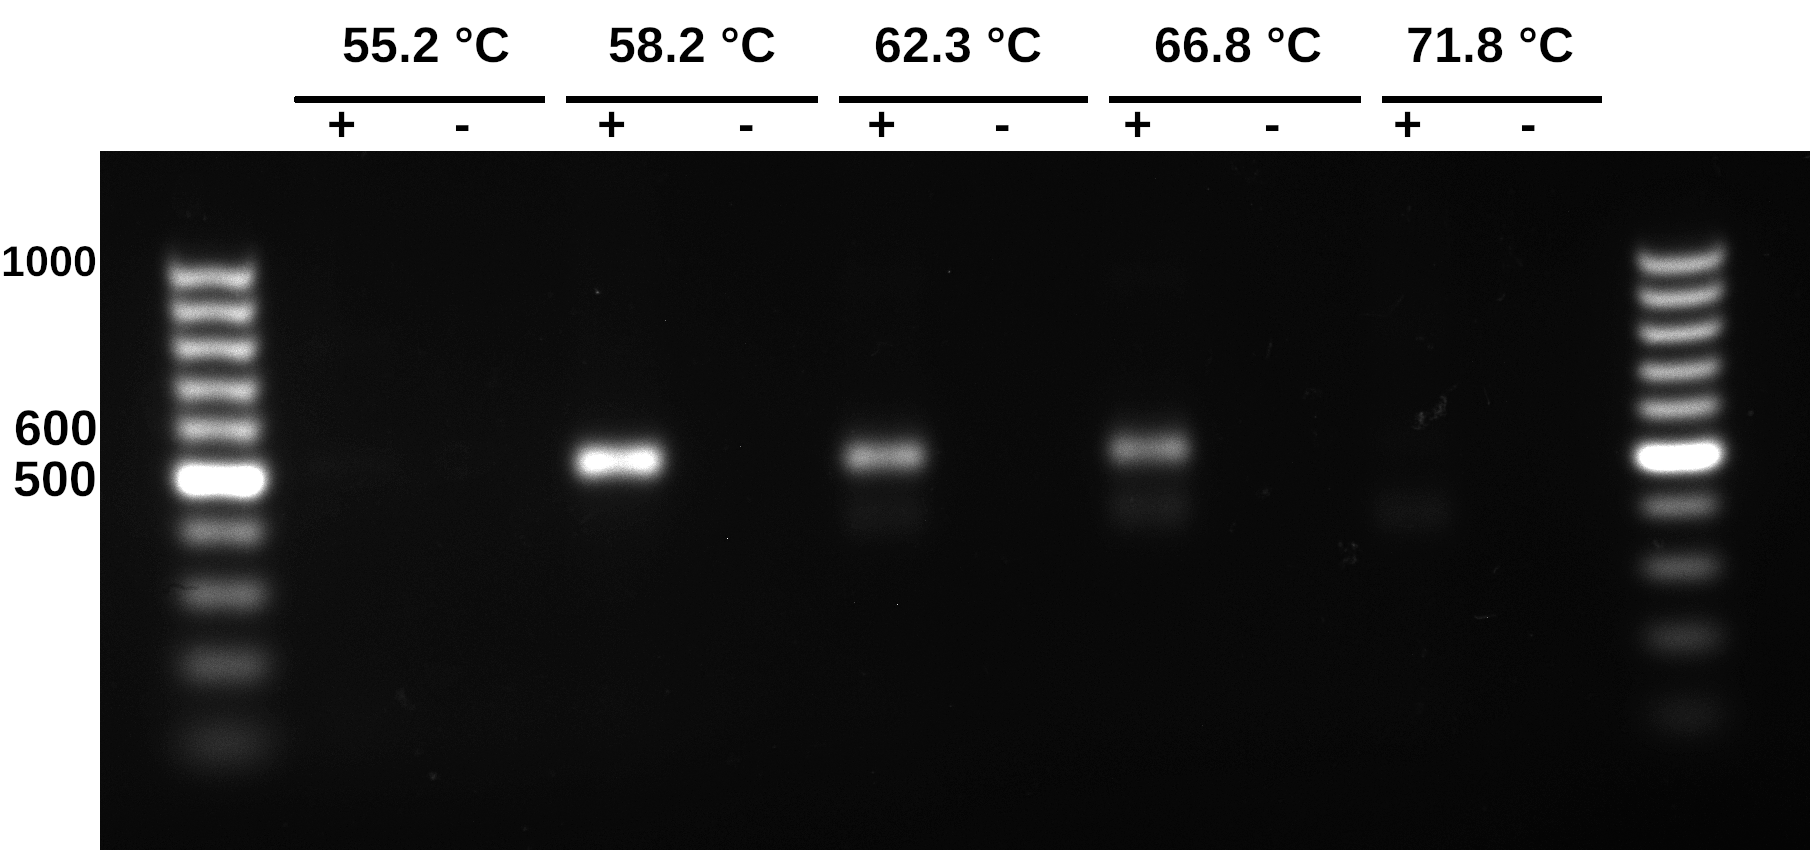
\includegraphics[width=0.95\textwidth]{figs/FigS2_Feb04-D RHA gradient PCR short elongation.png}
\label{figS2}
\caption{\textbf{Gradient PCR of D RHA fragment under different annealing temperature conditions shows optimal PCR parameters under a 19 second extension.} Lane order: GeneRuler 100bp, 55.2 \textdegree{}C, 55.2 \textdegree{}C n.c., 58.2 \textdegree{}C, 58.2 \textdegree{}C n.c., 62.3 \textdegree{}C, 62.3 \textdegree{}C n.c., 66.8 \textdegree{}C, 66.8 \textdegree{}C n.c., 71.8 \textdegree{}C, 71.8 \textdegree{}C n.c., GeneRuler 100bp. PCR products were visible for the middle three temperature settings, but were most pronounced at an annealing temperature of 58.2 \textdegree{}C.}
\end{figure}

\begin{figure}[htbp]
\centering
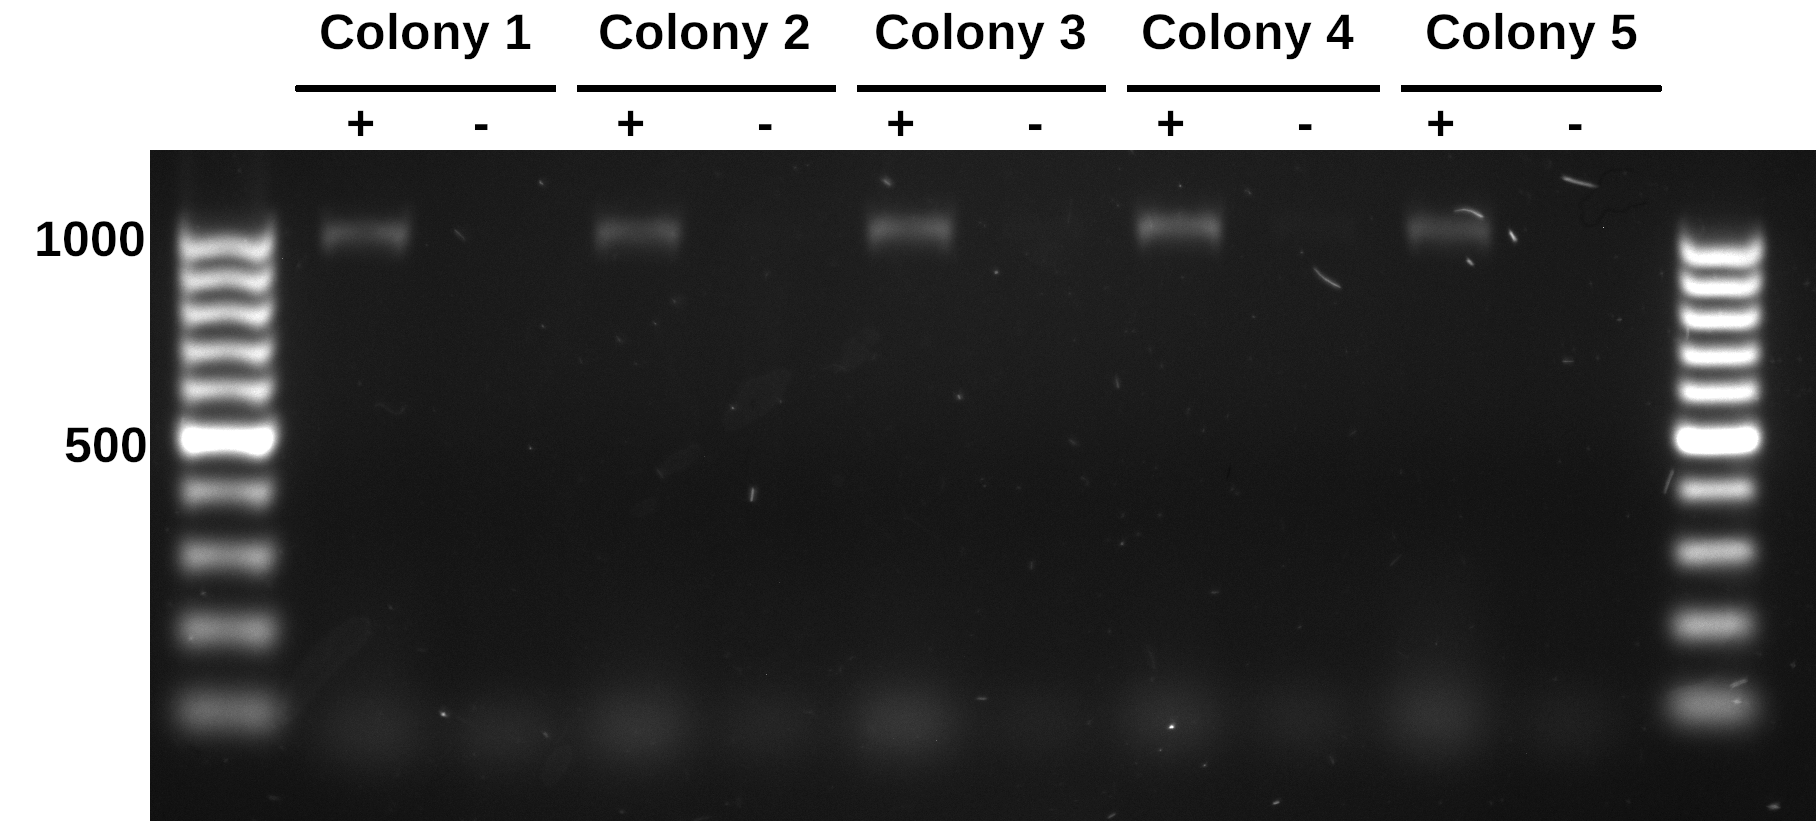
\includegraphics[width=0.95\textwidth]{figs/FigS3_Feb08-D colony PCR for Sox2 false positives.png}
\label{figS3}
\caption{\textbf{Colony PCR first-pass screen for mSox2 CDS fragment in ``Sox2 in D'' transformed colonies.} All five colonies appear to show a positive result for the presence of mSox2. Lane order: GeneRuler 100bp, Colony 1, Colony 1 n.c., Colony 2, Colony 2 n.c., Colony 3, Colony 3 n.c., Colony 4, Colony 4 n.c., Colony 5, Colony 5 n.c., GeneRuler 100bp}
\end{figure}

\begin{figure}[htbp]
\centering
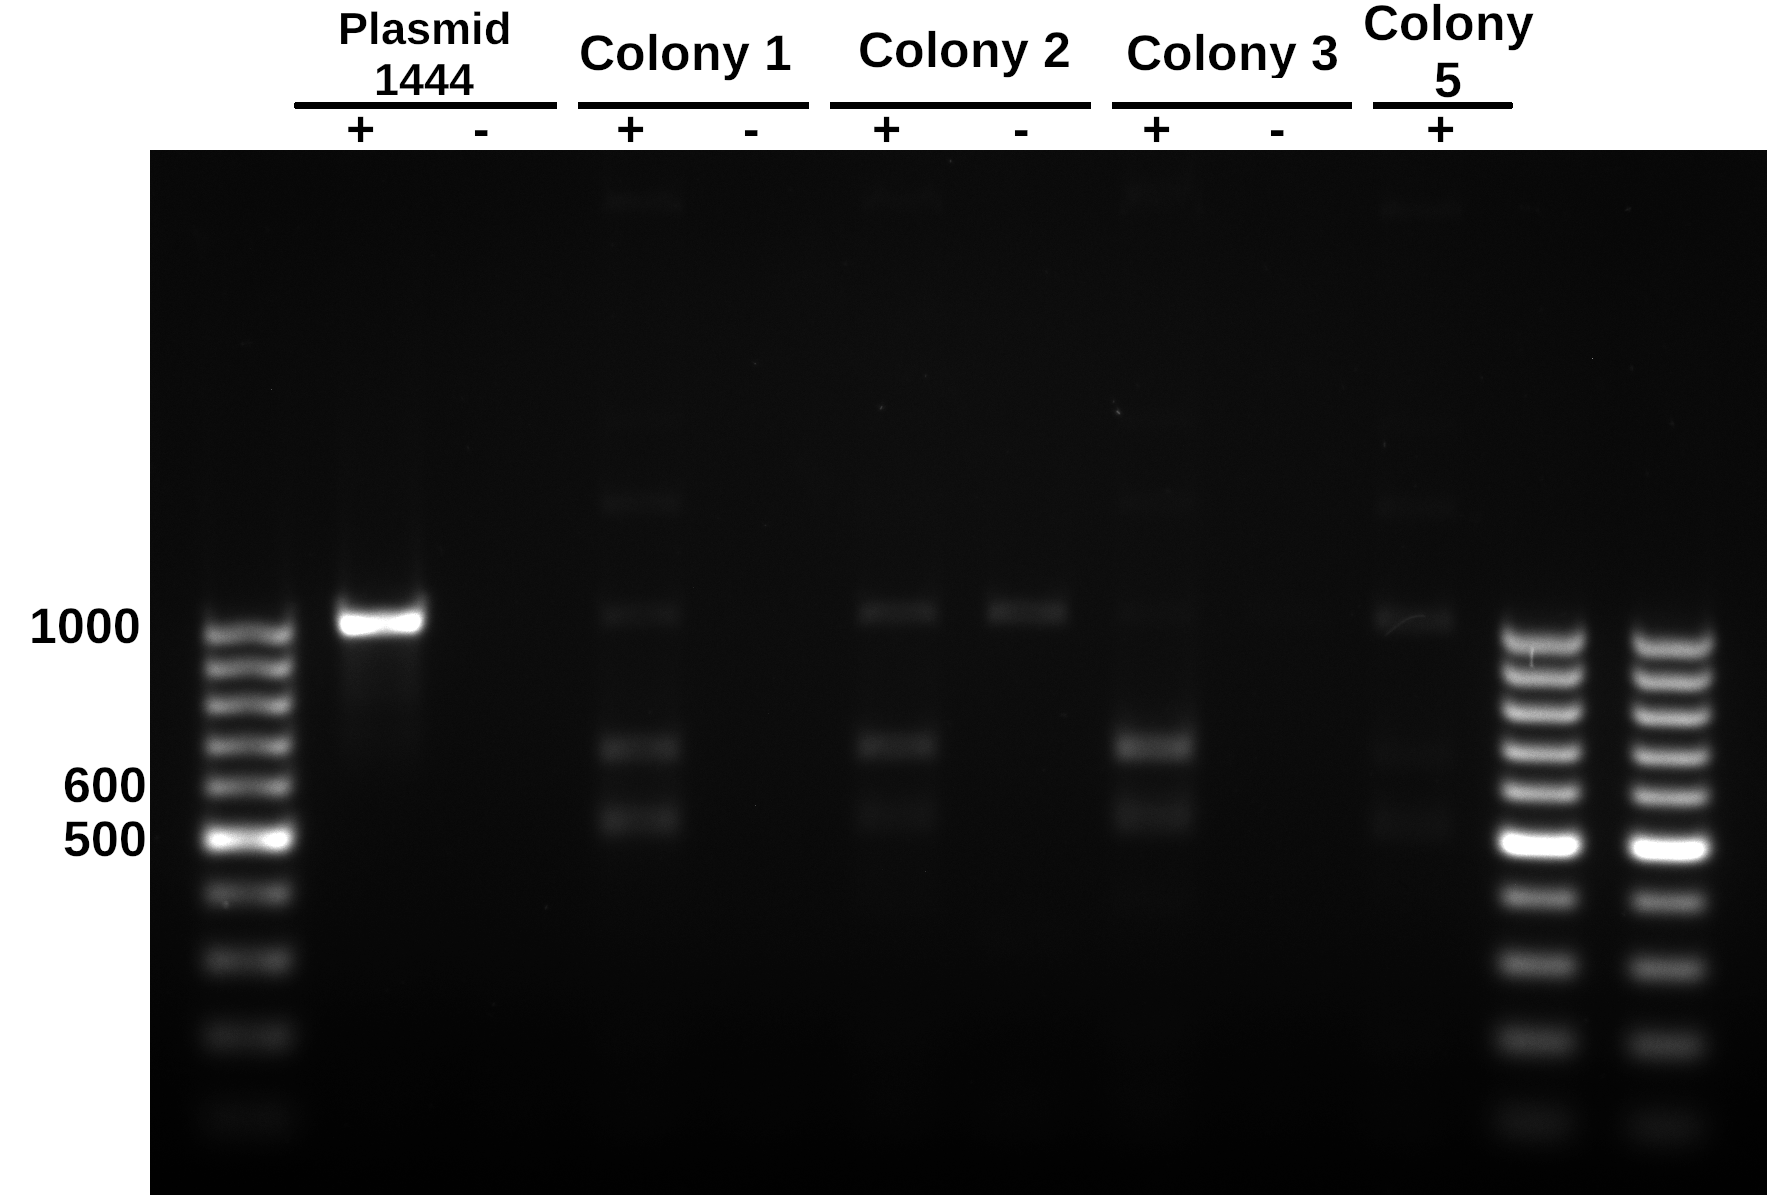
\includegraphics[width=0.95\textwidth]{figs/FigS4_Feb13-D colony frag 2 miniprepped PCR.png}
\label{figS4}
\caption{\textbf{PCR for mSox2 CDS fragment in purified DNA taken from ``Sox2 in D'' transformation colonies indicates high degree of false positives.} PCR of mSox2 sequence from plasmid 1444 is used as a positive control, with miniprepped plasmid DNA from colonies in Figure S3 as comparison. In all cases, there is a significant amount of nonspecific bands, faint specific bands, as well as some contamination in the negative control lane for colony 2. Lane order: GeneRuler 100bp, plasmid 1444 p.c., plasmid 1444 n.c., Colony 1, Colony 1 n.c., Colony 2, Colony 2 n.c., Colony 3, Colony 3 n.c., Colony 5, GeneRuler 100bp, GeneRuler 100bp}
\end{figure}

\newpage{}

\begin{landscape}
\begin{figure}[htbp]
\centering
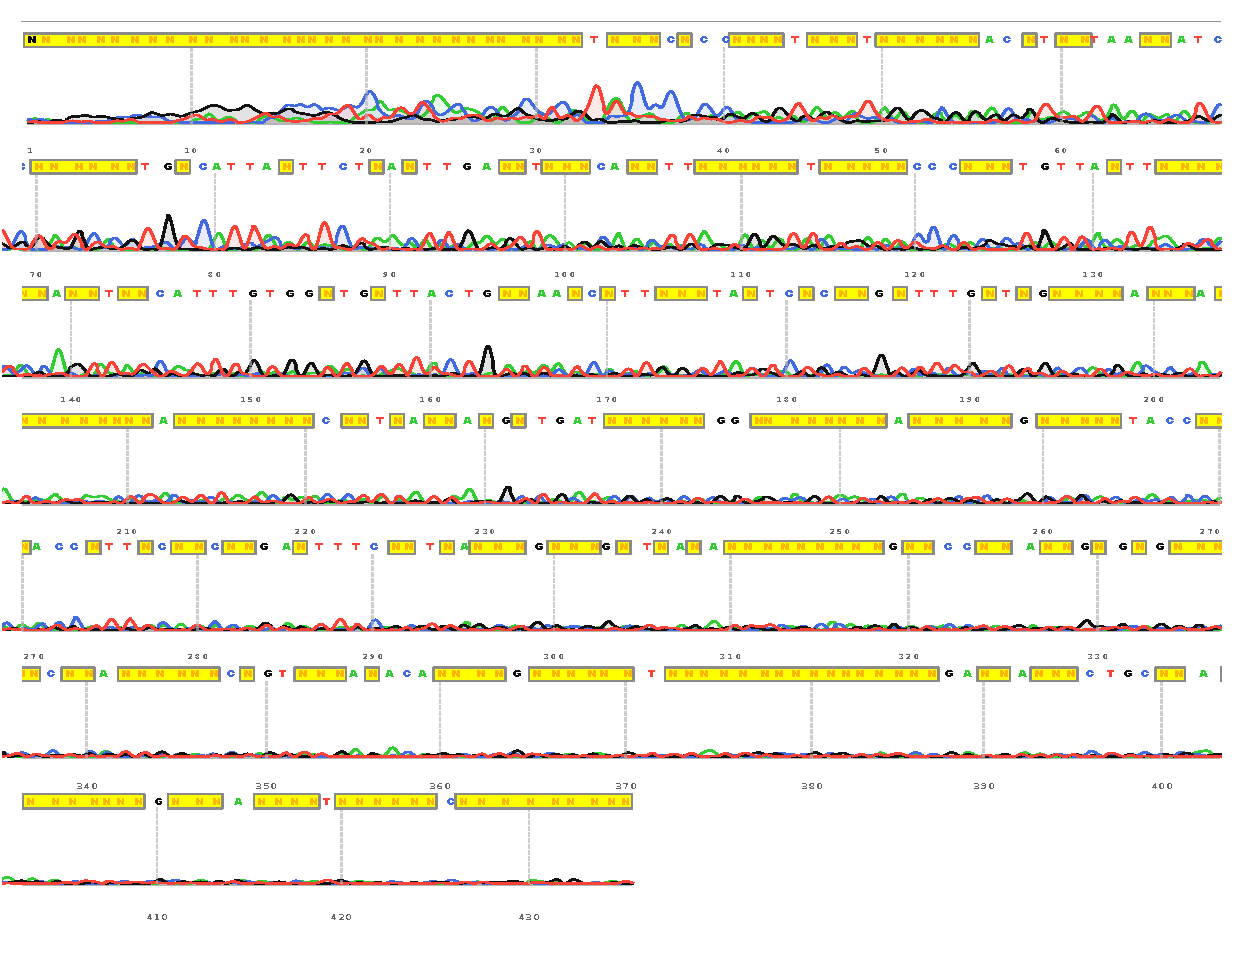
\includegraphics[width=0.76\linewidth]{figs/FigS5_SangerSequence.pdf}
\label{figS5}
\caption{\textbf{Sanger sequencing attempt with custom PCR primers for plasmid 1444 yields low-quality results.} Only 435 bases were reported despite the primers being 1375 bp apart, of which 282 bases were reported simply as ``N''. }
\end{figure}
\end{landscape}

\newpage{}

\makeatletter 
\renewcommand{\thetable}{S\@arabic\c@table}
\makeatother
\setcounter{table}{0}

\begin{landscape}

\begin{table}[]
\centering
\begin{adjustbox}{max width=\linewidth}
\begin{tabular}{|
>{\columncolor[HTML]{DAE8FC}}l 
>{\columncolor[HTML]{DAE8FC}}l 
>{\columncolor[HTML]{DAE8FC}}l 
>{\columncolor[HTML]{DAE8FC}}l |
>{\columncolor[HTML]{ECF4FF}}l 
>{\columncolor[HTML]{ECF4FF}}l |
>{\columncolor[HTML]{DAE8FC}}l 
>{\columncolor[HTML]{DAE8FC}}l |
>{\columncolor[HTML]{ECF4FF}}l 
>{\columncolor[HTML]{ECF4FF}}l 
>{\columncolor[HTML]{ECF4FF}}l 
>{\columncolor[HTML]{ECF4FF}}l |}
\hline
\multicolumn{4}{|c|}{\cellcolor[HTML]{0075c5}{\color[HTML]{FFFFFF} \textbf{SoxN-D Two Degrees of Separation}}} & \multicolumn{2}{c|}{\cellcolor[HTML]{0075c5}{\color[HTML]{FFFFFF} \textbf{Cluster A}}} & \multicolumn{2}{c|}{\cellcolor[HTML]{0075c5}{\color[HTML]{FFFFFF} \textbf{Cluster B}}} & \multicolumn{4}{c|}{\cellcolor[HTML]{0075c5}{\color[HTML]{FFFFFF} \textbf{Cluster C}}} \\ \hline
Aac11 & dnc & nmo & Saf-B & AcrE & PIP4K & Acn & Rbp1 & Ald & l(2)37Cc & RpL18 & Vha26 \\
Acn & eff & nSyb & SC35 & AP-1sigma & Pkc53E & B52 & Rbp1-like & ATPsynB & levy & RpL23A & Vha55 \\
arm & elav & onecut & scaf6 & cac & Pur-alpha & bl & Ref1 & ATPsynF & Mdh2 & RpL24 & Vha68-1 \\
B52 & Eph & pan & sd & CG4612 & qvr & bol & Rm62 & awd & Mpcp & RpL35A & VhaAC45 \\
beat-Ic & exd & para & SF2 & CG9132 & Rab11 & Caper & Rsf1 & bic & mRpL12 & RpL37a & VhaM8.9 \\
bl & fl(2)d & Pgk & sgg & comt & Rbp & CG10077 & Saf-B & blw & mRpL2 & RpL4 & VhaPPA1-1 \\
Bx & fne & Pka-C1 & shi & cpx & Rbp6 & CG31712 & SC35 & CG11752 & mRpL22 & RpL6 & vig \\
cac & FoxP & Pkc53E & snRNP70K & Crk & Rdl & CG3198 & scaf6 & CG11876 & mRpL4 & RpL8 &  \\
Caper & ftz-f1 & plum & Sox21b & Csp & Rim & CG7903 & SF2 & CG11984 & Nacalpha & RpLP0 &  \\
CG10077 & fz2 & pros & SoxN & Dap160 & Rop & CG7971 & snRNP70K & CG13220 & ND-18 & RpLP1 &  \\
CG12054 & Gad1 & ps & sqd & dor & shi & CG9775 & sqd & CG17065 & ND-30 & RpS10b &  \\
CG13220 & Gapdh1 & psq & svp & e(r) & slo & dod & stmA & CG42575 & ND-39 & RpS14a &  \\
CG13928 & gish & pUf68 & Syn & eag & Snap25 & fl(2)d & su(w{[}a{]}) & CG4300 & ND-75 & RpS14b &  \\
CG1677 & Gs1 & Rb97D & Syt1 & elav & Syn & fne & x16 & CG5214 & ND-B14.5A & RpS19a &  \\
CG32000 & HDAC4 & Rbp1 & tau & EndoA & Syngr & Hrb87F & YT521-B & CG5903 & ND-B17 & RpS2 &  \\
CG4328 & hig & Rbp1-like & Tpi & Gad1 & Synj & Hrb98DE &  & CG7215 & ND-B18 & RpS26 &  \\
CG5214 & His2Av & Rbp6 & vfl & gish & Syt1 & Inr-a &  & COX4 & Pgk & RpS8 &  \\
CG7967 & Hrb87F & Rdl & x16 & GluRIA & Syt4 & kcc &  & COX5A & Pglym78 & SdhA &  \\
CG7971 & Hrb98DE & Ref1 &  & GluRIB & Syx1A & La &  & Cyt-c1 & PyK & SdhB &  \\
chinmo & Hsc70-4 & RFeSP &  & lap & Syx6 & lark &  & Eno & Rack1 & SdhD &  \\
Crk & hth & Rm62 &  & Lerp & tau & Pep &  & Gapdh1 & ras & Sec61beta &  \\
crol & Inr-a & Rpn10 &  & nAChRbeta1 & Tomosyn & ps &  & Hsp60 & RFeSP & sta &  \\
Csp & Lar & Rpt3 &  & nonA & VGAT & pUf68 &  & l(1)G0156 & RpL13 & Tpi &  \\
CtBP & mam & Rpt4 &  & nSyb &  & qkr58E-1 &  & l(1)G0255 & RpL13A & UQCR-C1 &  \\
D & Mnn1 & Rsf1 &  & para &  & Rb97D &  & l(1)G0334 & RpL17 & UQCR-C2 &  \\ \hline
\end{tabular}
\end{adjustbox}
\caption{\textbf{Full gene list for sub-clusters within adult ventral nerve cord cluster 108.} Clusters A, B, and C represent the core genes for the three high-density areas within the GRN of cluster 108 (Figure 27). \emph{SoxN}, \emph{D}, and all genes within two degrees of separation are also included. Gene Ontology analysis reveals that these gene clusters are enriched for different biological processes. Cluster A is enriched for neurotransmission, Cluster B for mRNA processing, and Cluster C for translation and metabolism. The genes associated with \emph{SoxN} and \emph{D} are enriched for transcriptional regulation and functions related to clusters A-C.}
\end{table}

\end{landscape}

%%%%%%%%%%%%%%%%%%%%%%%%%%%%%%%%%%%%%%%%%%%%%%%%%%%%%%%%%%%%%%%%%%%%%%%%%%%%%%%%
%% Index:
%%
%\printthesisindex

\end{document}
